\documentclass{article}
\usepackage[backend=biber,natbib=true,style=alphabetic,maxbibnames=50]{biblatex}
\addbibresource{/home/nqbh/reference/bib.bib}
\usepackage[utf8]{vietnam}
\usepackage{tocloft}
\renewcommand{\cftsecleader}{\cftdotfill{\cftdotsep}}
\usepackage[colorlinks=true,linkcolor=blue,urlcolor=red,citecolor=magenta]{hyperref}
\usepackage{amsmath,amssymb,amsthm,enumitem,fancyvrb,float,graphicx,mathtools,multicol,soul,subfig,tikz}
\setlist[itemize]{leftmargin=*}
\usetikzlibrary{angles,calc,intersections,matrix,patterns,quotes,shadings}
\allowdisplaybreaks
\newtheorem{assumption}{Assumption}
\newtheorem{baitoan}{}
\newtheorem{cauhoi}{Câu hỏi}
\newtheorem{conjecture}{Conjecture}
\newtheorem{corollary}{Corollary}
\newtheorem{dangtoan}{Dạng toán}
\newtheorem{definition}{Definition}
\newtheorem{dinhly}{Định lý}
\newtheorem{dinhnghia}{Định nghĩa}
\newtheorem{example}{Example}
\newtheorem{ghichu}{Ghi chú}
\newtheorem{hequa}{Hệ quả}
\newtheorem{hypothesis}{Hypothesis}
\newtheorem{lemma}{Lemma}
\newtheorem{luuy}{Lưu ý}
\newtheorem{nhanxet}{Nhận xét}
\newtheorem{notation}{Notation}
\newtheorem{note}{Note}
\newtheorem{principle}{Principle}
\newtheorem{problem}{Problem}
\newtheorem{proposition}{Proposition}
\newtheorem{question}{Question}
\newtheorem{remark}{Remark}
\newtheorem{theorem}{Theorem}
\newtheorem{vidu}{Ví dụ}
\usepackage[left=1cm,right=1cm,top=5mm,bottom=5mm,footskip=4mm]{geometry}
\def\labelitemii{$\circ$}
\DeclareRobustCommand{\divby}{%
	\mathrel{\vbox{\baselineskip.65ex\lineskiplimit0pt\hbox{.}\hbox{.}\hbox{.}}}%
}

\title{Problem: Elementary Computer Science -- Bài Tập Tin Học Sơ Cấp}
\author{Nguyễn Quản Bá Hồng\footnote{A Scientist {\it\&} Creative Artist Wannabe. E-mail: {\tt nguyenquanbahong@gmail.com}. Bến Tre City, Việt Nam.}}
\date{\today}

\begin{document}
	\maketitle
\begin{abstract}
	This text is a part of the series {\it Some Topics in Elementary STEM \& Beyond}:
	
	{\sc url}: \url{https://nqbh.github.io/elementary_STEM}.
	
	Latest version:
	\begin{itemize}
		\item {\it Problems in Elementary Computer Science -- Bài Tập Tin Học Sơ Cấp}.
		
		PDF: {\sc url}: \url{https://github.com/NQBH/elementary_STEM_beyond/blob/main/elementary_computer_science/problem/NQBH_elementary_computer_science_problem.pdf}.
		
		\TeX: {\sc url}: \url{https://github.com/NQBH/elementary_STEM_beyond/blob/main/elementary_computer_science/problem/NQBH_elementary_computer_science_problem.tex}.
		\item {\it Problem \& Solution: Elementary Computer Science -- Bài Tập \& Lời Giải: Tin Học Sơ Cấp}.
		
		PDF: {\sc url}: \url{https://github.com/NQBH/elementary_STEM_beyond/blob/main/elementary_computer_science/problem/NQBH_elementary_computer_science_solution.pdf}.
		
		\TeX: {\sc url}: \url{https://github.com/NQBH/elementary_STEM_beyond/blob/main/elementary_computer_science/problem/NQBH_elementary_computer_science_solution.tex}.
	\end{itemize}
\end{abstract}
\tableofcontents

%------------------------------------------------------------------------------%

\subsection*{General structure -- Cấu trúc tổng quát}

\begin{baitoan}[General structure of a programming problem]
	(a) Viết thuật toán, vẽ lưu đồ, \& viết chương trình {\sf Pascal, Python, C{\tt/}C++} để:
	\begin{itemize}
		\item Tính
		\item Tìm
		\item Xác định
	\end{itemize}
	(b) Mở rộng \& tổng quát bài toán.
\end{baitoan}

\section{Basic -- Cơ Bản}

\subsection{Elementary algebra -- Đại số sơ cấp}

\begin{baitoan}[\cite{Doanh_Tuan_Pascal}, VD1, p. 14]
	(a) Cho $A = x^2 + y^2,B = x + y + A,C = xy + A - B^2$ với $x,y\in\mathbb{R}$. Tính $A,B,C$. (b) Mở rộng bài toán cho $A_i(x,y)\in\mathbb{R}[x,y]$ với $i = 1,2,\ldots,n$, $n\in\mathbb{N}^\star$, là các đa thức 2 biến $x,y$. (c) Mở rộng bài toán cho $A_i({\bf x})\in\mathbb{R}[{\bf x}]$ với $i = 1,2,\ldots,n$, là các đa thức  hệ số thực với $n\in\mathbb{N}^\star$ biến số ${\bf x} = (x_1,x_2,\ldots,x_n)$.
\end{baitoan}
See also:
\begin{itemize}
	\item {\it Problem: Algebraic Expression -- Bài Tập: Biểu Thức Đại Số}.
	
	Folder: {\sf Elementary STEM \& Beyond{\tt/}Elementary Mathematics{\tt/}grade 7{\tt/}algebraic expression{\tt/}problem}: [\href{https://github.com/NQBH/elementary_STEM_beyond/blob/main/elementary_mathematics/grade_7/algebraic_expression/problem/NQBH_algebraic_expression_problem.pdf}{pdf}\footnote{{\sc url}: \url{https://github.com/NQBH/elementary_STEM_beyond/blob/main/elementary_mathematics/grade_7/algebraic_expression/problem/NQBH_algebraic_expression_problem.pdf}.}][\href{https://github.com/NQBH/elementary_STEM_beyond/blob/main/elementary_mathematics/grade_7/algebraic_expression/problem/NQBH_algebraic_expression_problem.tex}{\TeX}\footnote{{\sc url}: \url{https://github.com/NQBH/elementary_STEM_beyond/blob/main/elementary_mathematics/grade_7/algebraic_expression/problem/NQBH_algebraic_expression_problem.tex}.}].
	\item {\it Problem \& Solution: Algebraic Expression -- Bài Tập \& Lời Giải: Biểu Thức Đại Số}.
	
	Folder: {\sf Elementary STEM \& Beyond{\tt/}Elementary Mathematics{\tt/}grade 7{\tt/}algebraic expression{\tt/}solution}: [\href{https://github.com/NQBH/elementary_STEM_beyond/blob/main/elementary_mathematics/grade_7/algebraic_expression/problem/NQBH_algebraic_expression_solution.pdf}{pdf}\footnote{{\sc url}: \url{https://github.com/NQBH/elementary_STEM_beyond/blob/main/elementary_mathematics/grade_7/algebraic_expression/problem/NQBH_algebraic_expression_solution.pdf}.}][\href{https://github.com/NQBH/elementary_STEM_beyond/blob/main/elementary_mathematics/grade_7/algebraic_expression/problem/NQBH_algebraic_expression_solution.tex}{\TeX}\footnote{{\sc url}: \url{https://github.com/NQBH/elementary_STEM_beyond/blob/main/elementary_mathematics/grade_7/algebraic_expression/problem/NQBH_algebraic_expression_solution.tex}.}].
\end{itemize}

\begin{baitoan}[\cite{Doanh_Tuan_Pascal}, VD2, p. 15]
	(a) Tìm {\rm GTLN} $\max\{a,b,c\}$ \& {\rm GTNN} $\min\{a,b,c\}$ với $a,b,c\in\mathbb{R}$. (b) Mở rộng bài toán cho $n\in\mathbb{N}^\star$ số $a_1,a_2,\ldots,a_n$.
\end{baitoan}

\begin{baitoan}[\cite{Doanh_Tuan_Pascal}, VD3, p. 16]
	(a) Tính giá trị của hàm số $f:\mathbb{R}^2\to\mathbb{R}$ xác định bởi công thức:
	\begin{equation*}
		f(x,y) = \left\{\begin{split}
			&x^3 + y^3&&\mbox{if }0\le x - y\le10,\\
			&x^2 + y^2&&\mbox{if } x - y < 0,\ y\ge0,\\
			&(x - y)^2&&\mbox{else}.
		\end{split}\right.
	\end{equation*}
	(b) Mở rộng bài toán cho các hàm số tương tự.
\end{baitoan}

\begin{baitoan}[\cite{Doanh_Tuan_Pascal}, VD4, p. 17]
	(a) Tìm nghiệm của phương trình bậc $\le2$ có dạng $ax^2 + bx + c = 0$ với $a,b,c\in\mathbb{R}$. (b) Mở rộng bài toán cho phương trình bậc 3, bậc 4. (c) Mở rộng bài toán cho các phương trình đa thức có thể giải được nhờ quy về phương trình bậc 2, 3.
\end{baitoan}
See also:
\begin{itemize}
	\item {\it Problem: 2nd-Order Function. Quadratic Equation -- Bài Tập: Hàm Số Bậc 2 $y = ax^2$. Phương Trình Bậc 2 1 Ẩn $ax^2 + bx + c = 0$}.
	
	Folder: {\sf Elementary STEM \& Beyond{\tt/}Elementary Mathematics{\tt/}grade 9{\tt/}2nd-order function, quadratic equation{\tt/}problem}: [\href{https://github.com/NQBH/elementary_STEM_beyond/blob/main/elementary_mathematics/grade_9/2nd_order_function/problem/NQBH_2nd_order_function_problem.pdf}{pdf}\footnote{{\sc url}: \url{https://github.com/NQBH/elementary_STEM_beyond/blob/main/elementary_mathematics/grade_9/2nd_order_function/problem/NQBH_2nd_order_function_problem.pdf}.}][\href{https://github.com/NQBH/elementary_STEM_beyond/blob/main/elementary_mathematics/grade_9/2nd_order_function/problem/NQBH_2nd_order_function_problem.tex}{\TeX}\footnote{{\sc url}: \url{https://github.com/NQBH/elementary_STEM_beyond/blob/main/elementary_mathematics/grade_9/2nd_order_function/problem/NQBH_2nd_order_function_problem.tex}.}].
	\item {\it Problem \& Solution: 2nd-Order Function. Quadratic Equation -- Bài Tập \& Lời Giải: Hàm Số Bậc 2 $y = ax^2$. Phương Trình Bậc 2 1 Ẩn $ax^2 + bx + c = 0$}.
	
	Folder: {\sf Elementary STEM \& Beyond{\tt/}Elementary Mathematics{\tt/}grade 9{\tt/}2nd-order function, quadratic equation{\tt/}solution}: [\href{https://github.com/NQBH/elementary_STEM_beyond/blob/main/elementary_mathematics/grade_9/2nd_order_function/solution/NQBH_2nd_order_function_solution.pdf}{pdf}\footnote{{\sc url}: \url{https://github.com/NQBH/elementary_STEM_beyond/blob/main/elementary_mathematics/grade_9/2nd_order_function/solution/NQBH_2nd_order_function_solution.pdf}.}][\href{https://github.com/NQBH/elementary_STEM_beyond/blob/main/elementary_mathematics/grade_9/2nd_order_function/solution/NQBH_2nd_order_function_solution.tex}{\TeX}\footnote{{\sc url}: \url{https://github.com/NQBH/elementary_STEM_beyond/blob/main/elementary_mathematics/grade_9/2nd_order_function/solution/NQBH_2nd_order_function_solution.tex}.}].
\end{itemize}

\begin{baitoan}[\cite{Doanh_Tuan_Pascal}, VD5, p. 18]
	Tính tổng $S = \sum_{i=1}^{100} x_i$ với $x_i\in\mathbb{R}$, $\forall i = 1,2,\ldots,100$. (b) Mở rộng bài toán cho các tổng tương tự.
\end{baitoan}

\begin{baitoan}[\cite{Doanh_Tuan_Pascal}, VD6, p. 19]
	Tính giá trị của đa thức $P(x) = \sum_{i=0}^n a_ix^i = a_nx^n + a_{n-1}x^{n-1} + \cdots + a_1x + a_0\in\mathbb{R}[x]$ với hệ số thực $a_i\in\mathbb{R}$, $\forall i = 0,1,\ldots,n$ với $n\in\mathbb{N}^\star$ bằng cách sử dụng thuật toán Horner.
\end{baitoan}

\begin{baitoan}[\cite{Doanh_Tuan_Pascal}, VD7, p. 21]
	Tính giá trị hàm số mũ $e^x$ với $x = a$ với sai số $\varepsilon > 0$ cho trước bằng cách sử dụng khai triển Taylor của hàm $e^x$.
\end{baitoan}

\begin{baitoan}[\cite{Doanh_Tuan_Pascal}, VD8, p. 22]
	Tìm nghiệm của phương trình $f(x) = x^5 - 6x^4 - 15x^3 - 20x^2 + 14x - 4 = 0$ với giá trị đầu (initial value) $x_0 = 0.8$.
\end{baitoan}

\begin{baitoan}[\cite{Doanh_Tuan_Pascal}, VD9, p. 23]
	Giải hệ phương trình tuyến tính cấp $n$ có dạng
	\begin{equation}
		\left\{\begin{split}
			a_{11}x_1 + a_{12}x_2 + \cdots + a_{1n}x_n &= b_1,\\
			a_{21}x_1 + a_{22}x_2 + \cdots + a_{2n}x_n &= b_2,\\
			&\vdots\\
			a_{n1}x_1 + a_{n2}x_2 + \cdots + a_{nn}x_n &= b_n.
		\end{split}\right.
	\end{equation}
\end{baitoan}
See also:
\begin{itemize}
	\item {\it Problem: System of 1st-Order Equations -- Bài Tập: Hệ Phương Trình Bậc Nhất $A{\bf x} = {\bf b}$}.
	
	Folder: {\sf Elementary STEM \& Beyond{\tt/}Elementary Mathematics{\tt/}grade 9{\tt/}system of 1st-order equations{\tt/}problem}: [\href{https://github.com/NQBH/elementary_STEM_beyond/blob/main/elementary_mathematics/grade_9/system_1st_order_equations/problem/NQBH_system_1st_order_equations_problem.pdf}{pdf}\footnote{{\sc url}: \url{https://github.com/NQBH/elementary_STEM_beyond/blob/main/elementary_mathematics/grade_9/system_1st_order_equations/problem/NQBH_system_1st_order_equations_problem.pdf}.}][\href{https://github.com/NQBH/elementary_STEM_beyond/blob/main/elementary_mathematics/grade_9/system_1st_order_equations/problem/NQBH_system_1st_order_equations_problem.tex}{\TeX}\footnote{{\sc url}: \url{https://github.com/NQBH/elementary_STEM_beyond/blob/main/elementary_mathematics/grade_9/system_1st_order_equations/problem/NQBH_system_1st_order_equations_problem.tex}.}].
	\item {\it Problem \& Solution: System of 1st-Order Equations -- Bài Tập \& Lời Giải: Hệ Phương Trình Bậc Nhất $A{\bf x} = {\bf b}$}.
	
	Folder: {\sf Elementary STEM \& Beyond{\tt/}Elementary Mathematics{\tt/}grade 9{\tt/}system of 1st-order equations{\tt/}solution}: [\href{https://github.com/NQBH/elementary_STEM_beyond/blob/main/elementary_mathematics/grade_9/system_1st_order_equations/solution/NQBH_system_1st_order_equations_solution.pdf}{pdf}\footnote{{\sc url}: \url{https://github.com/NQBH/elementary_STEM_beyond/blob/main/elementary_mathematics/grade_9/system_1st_order_equations/solution/NQBH_system_1st_order_equations_solution.pdf}.}][\href{https://github.com/NQBH/elementary_STEM_beyond/blob/main/elementary_mathematics/grade_9/system_1st_order_equations/solution/NQBH_system_1st_order_equations_solution.tex}{\TeX}\footnote{{\sc url}: \url{https://github.com/NQBH/elementary_STEM_beyond/blob/main/elementary_mathematics/grade_9/system_1st_order_equations/solution/NQBH_system_1st_order_equations_solution.tex}.}].
	\item Problem: Trigonometry in Triangles -- Bài Tập: Hệ Thức Lượng Trong Tam Giác. {\sc url}: \url{https://github.com/NQBH/elementary_STEM_beyond/blob/main/elementary_mathematics/grade_9/trigonometry/problem/NQBH_trigonometry_problem.pdf}.
\end{itemize}

\begin{baitoan}[\cite{Doanh_Tuan_Pascal}, 10., p. 27]
	Tính tổ hợp chập $k$ trong $n$ phần tử $C_n^k$.
\end{baitoan}

\begin{baitoan}[\cite{Doanh_Tuan_Pascal}, 11., p. 27]
	Tính tích của $n$ số thực $x_1,x_2,\ldots,x_n\in\mathbb{R}$.
\end{baitoan}

\begin{baitoan}[\cite{Doanh_Tuan_Pascal}, 12., p. 27]
	Tính giá trị của biểu thức $A = \sum_{i=1}^{100} x_i + \prod_{i=1}^{100} x_i$.
\end{baitoan}

\begin{baitoan}[\cite{Doanh_Tuan_Pascal}, 13., p. 27]
	Xác định các số dương trong chuỗi số $x_1,x_2,\ldots,x_n$.
\end{baitoan}

\begin{baitoan}[\cite{Doanh_Tuan_Pascal}, 14., p. 27]
	Tính trung bình số học của các phần tử trong chuỗi số $x_1,x_2,\ldots,x_n$ trong đoạn $[a,b]$ với $a,b\in\mathbb{R}$, $a < b$.
\end{baitoan}

\begin{baitoan}[\cite{Doanh_Tuan_Pascal}, 15., p. 27]
	Tính $100$ số Fibonacci đầu tiên.
\end{baitoan}

\begin{baitoan}[\cite{Doanh_Tuan_Pascal}, 16., p. 27]
	Tìm số lớn nhất trong dãy số $x_1,x_2,\ldots,x_n$.
\end{baitoan}

\begin{baitoan}[\cite{Doanh_Tuan_Pascal}, 17., p. 27]
	Tính các phần tử của tam giác Pascal tới $C_{100}^{100}$.
\end{baitoan}

\begin{baitoan}[\cite{Doanh_Tuan_Pascal}, 18., p. 27]
	Gọi $x_1,x_2,\ldots,x_n$ là lượng cholesterol trung bình của người đến khám bệnh. Người khỏe có lượng cholesterol nhỏ hơn tiêu chuẩn $x < A$. Xác định số người không mắc bệnh \& lượng colesterol trung bình của người bệnh.
\end{baitoan}

\begin{baitoan}[\cite{Doanh_Tuan_Pascal}, 19., p. 27]
	Viết các hoán vị với 5 số $1,2,3,4,5$.
\end{baitoan}

\begin{baitoan}[\cite{Doanh_Tuan_Pascal}, 20., p. 27]
	Xếp các số theo thứ tự tăng dần hoặc giảm dần.
\end{baitoan}

\begin{baitoan}[\cite{Doanh_Tuan_Pascal}, 21., p. 27]
	Lập danh bạ điện thoại 5 số.
\end{baitoan}

\begin{baitoan}[\cite{Doanh_Tuan_Pascal}, 22., p. 27]
	Cho $a,b,c > 0$ bất kỳ. Nếu 3 số đó có thể là chiều dài 3 cạnh của 1 tam giác, tính chu vi \& diện tích tam giác đó.
\end{baitoan}

\begin{baitoan}[\cite{Doanh_Tuan_Pascal}, 23., p. 28]
	Tính $n!$ với $n\in\mathbb{Z}$.
\end{baitoan}

\begin{baitoan}[\cite{Doanh_Tuan_Pascal}, 24., p. 28]
	Tìm ước chung lớn nhất {\rm ƯCLN} của 2 số.
\end{baitoan}

\begin{baitoan}
	Tìm bội chung nhỏ nhất {\rm BCNN} của 2 hay nhiều số.
\end{baitoan}

\begin{baitoan}[\cite{Doanh_Tuan_Pascal}, 25., p. 28]
	Tính tổng \& tích của 1 chuỗi số biết giá trị đầu \& số các số hạng của chuỗi.
\end{baitoan}

\begin{baitoan}[\cite{Doanh_Tuan_Pascal}, 26., p. 28]
	Tính tổng của chuỗi $\sum_{i=1}^n \frac{1}{i} = 1 + \frac{1}{2} + \cdots + \frac{1}{n}$.
\end{baitoan}

\begin{baitoan}[\cite{Doanh_Tuan_Pascal}, 27., p. 28]
	Xác định các số nguyên tố trong đoạn $[1,n]$ với $n\in\mathbb{N}$ cho trước.
\end{baitoan}

\begin{baitoan}[\cite{Doanh_Tuan_Pascal}, 28., p. 28]
	Tính $y = \log_a x$ với cơ số $a > 0$ bất kỳ.
\end{baitoan}

%------------------------------------------------------------------------------%

\subsection{Vector, matrix, system of algebraic equations -- Vector, ma trận, hệ phương trình đại số}

\begin{baitoan}[\cite{Doanh_Tuan_Pascal}, 29., p. 28]
	Thực hiện phép cộng, trừ, tích vô hướng, tích vector đối với 2 vector trong không gian 3 chiều.
\end{baitoan}

\begin{baitoan}[\cite{Doanh_Tuan_Pascal}, 30., p. 28]
	Tính tích vô hướng của 2 vector $n$ chiều ${\bf x} = (x_1,x_2,\ldots,x_n),{\bf y} = (y_1,y_2,\ldots,y_n)$.
\end{baitoan}

\begin{baitoan}[\cite{Doanh_Tuan_Pascal}, 31., p. 28]
	Cho 2 vector $n$ chiều ${\bf x} = (x_1,x_2,\ldots,x_n),{\bf y} = (y_1,y_2,\ldots,y_n)$. Tính vector ${\bf z} = (z_1,z_2,\ldots,z_n)$ có các thành phần được xác định như sau:
	\begin{equation*}
		z_i = \left\{\begin{split}
			&0&&\mbox{if } 0 < x_i + y_i < a,\\
			&x_i + y_i&&\mbox{if } x_i + y_i\ge a,\\
			&(x_i + y_i)^2&&\mbox{if } x_i + y_i\le0,
		\end{split}\right.\ \forall i = 1,2,\ldots,n,
	\end{equation*}
	\& tích tích vô hướng ${\bf x}\cdot{\bf z}$.
\end{baitoan}

\begin{baitoan}[\cite{Doanh_Tuan_Pascal}, 32., p. 28]
	Tính ma trận chuyển vị của ma trận $A = (a_{ij})_{i,j=1}^{m,n}$.
\end{baitoan}

\begin{baitoan}[\cite{Doanh_Tuan_Pascal}, 33., p. 28]
	Xác định phần tử lớn nhất \& phần tử nhỏ nhất trong ma trận $A = (a_{ij})_{i,j=1}^{m,n}$.
\end{baitoan}

\begin{baitoan}[\cite{Doanh_Tuan_Pascal}, 34., p. 28]
	Tìm ma trận tổng $C = A + B$.
\end{baitoan}

\begin{baitoan}[\cite{Doanh_Tuan_Pascal}, 35., p. 28]
	Tìm ma trận tích $C = AB$.
\end{baitoan}

\begin{baitoan}[\cite{Doanh_Tuan_Pascal}, 36., p. 28]
	Tính định thức $D$ của hệ phương trình tuyến tính bậc $n\in\mathbb{N}^\star$.
\end{baitoan}

\begin{baitoan}[\cite{Doanh_Tuan_Pascal}, 37a., p. 28]
	Tính ma trận nghịch đảo.
\end{baitoan}

\begin{baitoan}[\cite{Doanh_Tuan_Pascal}, 37b., p. 28]
	Giải hệ phương trình đại số tuyến tính bậc $n\in\mathbb{N}^\star$ bằng phương pháp khử Gauss.
\end{baitoan}

%------------------------------------------------------------------------------%

\subsection{Function -- Hàm số}

\begin{baitoan}[\cite{Doanh_Tuan_Pascal}, 38., p. 29]
	Vẽ đồ thị hàm số theo từng điểm.
\end{baitoan}

\begin{baitoan}[\cite{Doanh_Tuan_Pascal}, 39., p. 29]
	Vẽ đồ thị hàm số, thực hiện dịch chuyển tọa độ \& vẽ các điểm.
\end{baitoan}

\begin{baitoan}[\cite{Doanh_Tuan_Pascal}, 40., p. 29]
	Xác định hàm số theo đồ thị hàm số.
\end{baitoan}

\begin{baitoan}[\cite{Doanh_Tuan_Pascal}, 41., p. 29]
	Tính giá trị liên tiếp của hàm số $y_i = \sin e^{x_i}$ trong đó $x_i\coloneqq a + i(b - a)$, $i = 1,2,\ldots,100$ với $a,b\in\mathbb{R}$ cho trước.
\end{baitoan}

\begin{baitoan}[\cite{Doanh_Tuan_Pascal}, 42., p. 29]
	Tính các giá trị của hàm số $y_i = e^{x_i} + \sin x_i$ với $x_i = a + hi$, $i = 1,2,\ldots,n$.
\end{baitoan}

\begin{baitoan}[\cite{Doanh_Tuan_Pascal}, 43., p. 29]
	Tính $\sqrt[n]{x}$.
\end{baitoan}

\begin{baitoan}[\cite{Doanh_Tuan_Pascal}, 44., p. 29]
	Lập chương trình tính toán các lượng phức: cộng, trừ, nhân, chia, lũy thừa các số phức.
\end{baitoan}

\begin{baitoan}[\cite{Doanh_Tuan_Pascal}, 45., p. 29]
	Lập chương trình đổi radian ra độ.
\end{baitoan}

\begin{baitoan}[\cite{Doanh_Tuan_Pascal}, 46., p. 29]
	Lập chương trình đổi độ ra radian.
\end{baitoan}

\begin{baitoan}[\cite{Doanh_Tuan_Pascal}, 47., p. 29]
	Tính giá trị của 2 hàm số $\sinh x,\cosh x$.
\end{baitoan}

\begin{baitoan}[\cite{Doanh_Tuan_Pascal}, 48., p. 29]
	Tính giá trị hàm số $y = a^x$.
\end{baitoan}

%------------------------------------------------------------------------------%

\subsection{Polynomials, interpolation polynomials -- Đa thức, đa thức nội suy}

\begin{baitoan}[\cite{Doanh_Tuan_Pascal}, 49., p. 29]
	Tính giá trị của đa thức Chevbyshev bậc $n\in\mathbb{N}^\star$
	\begin{align*}
		T_n(x)&\coloneqq\cos(n\arccos x),\\
		U_n(x)&\coloneqq\frac{\sin((n + 1)\arccos x)}{2^n\sqrt{1 - x^2}}.
	\end{align*}
\end{baitoan}

\begin{baitoan}[\cite{Doanh_Tuan_Pascal}, 50., p. 29]
	Tính giá trị của đa thức Legendre bậc $n\in\mathbb{N}^\star$
	\begin{equation*}
		L_n(x) = A_n\sum_{k=0}^{\lfloor n\rfloor} (-1)^k\frac{(2n - 2k)!}{(n - 2k)!}C_n^kx^{n - k}.
	\end{equation*}
\end{baitoan}

\begin{baitoan}[\cite{Doanh_Tuan_Pascal}, 51., p. 29]
	Tính giá trị của đa thức Laguerre:
	\begin{equation*}
		L_n^\alpha(x) = (-1)^nx^{-\alpha}e^x\frac{d^n}{dx^n}(x^{\alpha + n}e^{-x}).
	\end{equation*}
\end{baitoan}

\begin{baitoan}[\cite{Doanh_Tuan_Pascal}, 52., p. 30]
	Tính giá trị của đa thức Hermite:
	\begin{equation}
		H_n(x) = (-1)^ne^{\frac{x^2}{2}}\frac{d^n}{dx^n}e^{\frac{x^2}{2}}.
	\end{equation}
\end{baitoan}

\begin{baitoan}[\cite{Doanh_Tuan_Pascal}, 53., p. 30]
	Cho bảng các giá trị $(x_i,y_i)$. Tìm đa thức nội suy Lagrange.
\end{baitoan}

\begin{baitoan}[\cite{Doanh_Tuan_Pascal}, 54., p. 30]
	Cho bảng các giá trị $(x_i,y_i)$. Tìm ma trận nội suy Lagrange.
\end{baitoan}

\begin{baitoan}[\cite{Doanh_Tuan_Pascal}, 55., p. 30]
	Tìm đa thức nội suy Newton. Tính giá trị của đa thức nội suy tại điểm $x_0$ theo công thức Newton.
\end{baitoan}

\begin{baitoan}[\cite{Doanh_Tuan_Pascal}, 56., p. 30]
	Xác định trị số của đa thức nội suy tại điểm $x_0$ theo công thức Horner.
\end{baitoan}

\begin{baitoan}[\cite{Doanh_Tuan_Pascal}, 57., p. 30]
	Tính tổng 2 đa thức.
\end{baitoan}

\begin{baitoan}[\cite{Doanh_Tuan_Pascal}, 58., p. 30]
	Nhân 2 đa thức.
\end{baitoan}

\begin{baitoan}[\cite{Doanh_Tuan_Pascal}, 59., p. 30]
	Chia 2 đa thức.
\end{baitoan}

%------------------------------------------------------------------------------%

\subsection{Differentiation \& derivative -- Phép tính vi phân \& đạo hàm}

\begin{baitoan}[\cite{Doanh_Tuan_Pascal}, 60., p. 30]
	Tìm đạo hàm cấp $m\in\mathbb{N}$ của đa thức $P(x)$.
\end{baitoan}

\begin{baitoan}[\cite{Doanh_Tuan_Pascal}, 61., p. 30]
	Tìm đạo hàm cấp $m\in\mathbb{N}$ của đa thức nội suy Newton.
\end{baitoan}

\begin{baitoan}[\cite{Doanh_Tuan_Pascal}, 62., p. 30]
	Tìm đạo hàm 1 biến.
\end{baitoan}

\begin{baitoan}[\cite{Doanh_Tuan_Pascal}, 63., p. 30]
	Tìm gradient $\nabla$ hàm nhiều biến.
\end{baitoan}

\begin{baitoan}[\cite{Doanh_Tuan_Pascal}, 64., p. 30]
	Tìm giá trị của đạo hàm cấp $m\in\mathbb{N}$ của đa thức $P(x)$ tại điểm $x_0\in\mathbb{R}$.
\end{baitoan}

\begin{baitoan}[\cite{Doanh_Tuan_Pascal}, 65., p. 30]
	Tìm đạo hàm cấp 2 của hàm theo $x_ix_j$ tại 1 điểm theo công thức đạo hàm có bước biến đổi \& 1 quá trình ngoại suy.
\end{baitoan}

%------------------------------------------------------------------------------%

\subsection{Integration \& integral -- Phép tính tích phân \& tích phân}

\begin{baitoan}[\cite{Doanh_Tuan_Pascal}, 66., p. 30]
	Tính tích phân xác định bằng phương pháp Simpson.
\end{baitoan}

\begin{baitoan}[\cite{Doanh_Tuan_Pascal}, 67., p. 30]
	Tính tích phân xác định bằng phương pháp hình thang.
\end{baitoan}

\begin{baitoan}[\cite{Doanh_Tuan_Pascal}, 68., p. 30]
	Tính tích phân kép trong miền $D$ bằng phương pháp Gauss--Legendre.
\end{baitoan}

\begin{baitoan}[\cite{Doanh_Tuan_Pascal}, 69., p. 30]
	Tính tích phân kép bằng phương pháp Romberg.
\end{baitoan}

%------------------------------------------------------------------------------%

\subsection{Nonlinear system -- Phương trình phi tuyến}

\begin{baitoan}[\cite{Doanh_Tuan_Pascal}, 70., p. 31]
	Giải phương trình phi tuyến bằng phương pháp chia đôi cung.
\end{baitoan}

\begin{baitoan}[\cite{Doanh_Tuan_Pascal}, 71., p. 31]
	Giải phương trình phi tuyến bằng phương pháp lặp cát tuyến.
\end{baitoan}

\begin{baitoan}[\cite{Doanh_Tuan_Pascal}, 72., p. 31]
	Giải phương trình phi tuyến bằng phương pháp lặp Newton.
\end{baitoan}

%------------------------------------------------------------------------------%

\subsection{Optimization -- Tối ưu hóa}

\begin{baitoan}[\cite{Doanh_Tuan_Pascal}, 73., p. 31]
	Tìm cực trị của hàm số bằng phương pháp tiết diện vàng.
\end{baitoan}

\begin{baitoan}[\cite{Doanh_Tuan_Pascal}, 74., p. 31]
	Tìm cực trị của hàm nhiều biến bằng phương pháp gradient.
\end{baitoan}

\begin{baitoan}[\cite{Doanh_Tuan_Pascal}, 75., p. 31]
	Tìm cực trị của hàm 1 biến.
\end{baitoan}

%------------------------------------------------------------------------------%

\subsection{Differential equations -- Phương trình vi phân}

\begin{baitoan}[\cite{Doanh_Tuan_Pascal}, 76., p. 31]
	Giải phương trình vi phân bằng phương pháp Euler \& Euler cải tiến.
\end{baitoan}

\begin{baitoan}[\cite{Doanh_Tuan_Pascal}, 77., p. 31]
	Giải phương trình tích phân bằng phương pháp Romberg.
\end{baitoan}

\begin{baitoan}[\cite{Doanh_Tuan_Pascal}, 78., p. 31]
	Giải phương trình vi phân bằng phương pháp Runge--Kutta.
\end{baitoan}

\begin{baitoan}[\cite{Doanh_Tuan_Pascal}, 79., p. 31]
	Giải hệ phương trình vi phân cấp $n\in\mathbb{N}^\star$ bằng phương pháp Runge--Kutta.b
\end{baitoan}

%------------------------------------------------------------------------------%

\subsection{Probability \& Statistics -- Xác suất \& Thống kê}

\begin{baitoan}[\cite{Doanh_Tuan_Pascal}, 80., p. 31]
	Tìm phân bố nhị thức biết số phép thử $n = 10$, xác suất xuất hiện biến cố ngẫu nhiên trong mỗi phép thử là $p = 0.45$, $x = 4$.
\end{baitoan}

\begin{baitoan}[\cite{Doanh_Tuan_Pascal}, 81., p. 31]
	Dùng luật phân bố Poisson để tính trong $1000$ trang sách có $100$ lỗi in sai, tính xác suất để khi lấy ngẫu nhiên 1 trang có không quá $4$ lỗi.
\end{baitoan}

\begin{baitoan}[\cite{Doanh_Tuan_Pascal}, 82., p. 31]
	Biến ngẫu nhiên $x_i$ có xác suất $p_i$ cho bằng bảng phân bố $x_i,p_i$. Tìm kỳ vọng, phương sai, độ lệch bình phương trung bình, lấy $a = 2$.
\end{baitoan}

\begin{baitoan}[\cite{Doanh_Tuan_Pascal}, 83., pp. 31--32]
	Xác định hệ số tương quan giữa 2 biến ngẫu nhiên $x,y$. Kiểm tra xem mối liên hệ giữa $x,y$ có đủ tin cậy không.
\end{baitoan}

%------------------------------------------------------------------------------%

\subsection{Document managing \& processing -- Quản lý \& xử lý văn bản}

\begin{baitoan}[\cite{Doanh_Tuan_Pascal}, 84., p. 32]
	Lập chương trình in các ngày trong 1 tuần lễ.
\end{baitoan}

\begin{baitoan}[\cite{Doanh_Tuan_Pascal}, 85., p. 32]
	Lập chương trình in lịch thế kỷ.
\end{baitoan}

\begin{baitoan}[\cite{Doanh_Tuan_Pascal}, 86., p. 32]
	Quản lý 1 file nhập dữ liệu bằng bảng.
\end{baitoan}

\begin{baitoan}[\cite{Doanh_Tuan_Pascal}, 87., p. 32]
	Lập chương trình tìm kiếm 1 phần tử trong 1 danh sách.
\end{baitoan}

\begin{baitoan}[\cite{Doanh_Tuan_Pascal}, 88., p. 32]
	Lập chương trình làm 1 tờ hóa đơn.
\end{baitoan}

\begin{baitoan}[\cite{Doanh_Tuan_Pascal}, 89., p. 32]
	Lập chương trình quản lý danh sách cán bộ.
\end{baitoan}

\begin{baitoan}[\cite{Doanh_Tuan_Pascal}, 90., p. 32]
	Lập chương trình in danh sách cán bộ.
\end{baitoan}

\begin{baitoan}[\cite{Doanh_Tuan_Pascal}, 91., p. 32]
	Quản lý 1 file nhập dữ liệu bằng con trỏ.
\end{baitoan}

%------------------------------------------------------------------------------%

\subsection{Technology -- Bài toán kỹ thuật}

\begin{baitoan}[\cite{Doanh_Tuan_Pascal}, 92., p. 32]
	Tính đặc tính tần số của tổng trở, góc pha, dòng điện, \& điện áp trên các phần tử của mạch R-L-C nối tiếp.
\end{baitoan}

\begin{baitoan}[\cite{Doanh_Tuan_Pascal}, Chế độ quá độ trong 1 điện trở đốt nóng, 97., p. 35]
	 1 điện trở kim loại có hệ số nhiệt $\rm\alpha = 10^{-3}K^{-1}$. Trong miền nhiệt độ $T$, điện trở phụ thuộc vào nhiệt độ theo quy luật $R = R_0(1 + \alpha(T - T_0))$. Điện trở truyền công suất nhiệt vào 1 môi trường xung quanh có nhiệt độ $T_0$: $P_T = G(T - T_0)$; nhiệt dung $C$ của điện trở là $\rm2JK^{-1}$. Giả thiết nhiệt độ là đều ở mỗi thời điểm, điện áp đặt vào điện trở là $U = 220$ {\rm V}. Tại thời điểm $t = 0$ nhiệt độ bằng nhiệt độ môi trường $T_0 = 300$ {\rm K}, đặt $\theta = T - T_0$. (a) Viết phương trình vi phân của hàm $\theta(t)$. (b) Khi đạt tới chế độ xác lập ta đo được nhiệt độ {\rm800 K} \& công suất tiêu tán {\rm500 W}. Xác định trị số $R_0,G$. (c) Giải phương trình vi phân bằng phương pháp số. Chọn bước sao cho kết quả chính xác với 2 chữ số. Xác định nhiệt độ ở mỗi giây từ {\rm0--10 s}. So sánh với các kết quả thu được khi cho rằng ngay lúc đầu điện trở có giá trị cuối.
\end{baitoan}
\textit{Các bài toán không được trình bày do bao gồm hình vẽ khá phức tạp}: \cite[93., 94., 95., 96., 98., 99., 100., 101., pp. 32--38]{Doanh_Tuan_Pascal}. Bạn đọc tìm đến sách này để tham khảo thêm.

%------------------------------------------------------------------------------%

\section{Number Theory -- Số Học}

\begin{baitoan}[\cite{Huy_sang_tao_thuat_toan_lap_trinh_tap_1}, p. 6, số thân thiện -- friendly number]
	(a) Tìm tất cả các số tự nhiên có 2 chữ số mà khi đảo trật tự của 2 chữ số đó sẽ thu được 1 số nguyên tố cùng nhau với số đã cho. (b) Mở rộng bài toán cho số tự nhiên có $n$ chữ số với $n\in\mathbb{N},n\ge2$.
\end{baitoan}

\begin{baitoan}[\cite{Huy_sang_tao_thuat_toan_lap_trinh_tap_1}, p. 13, cấp số cộng -- arithmetic progression]
	(a) Tìm các số tự nhiên lẻ gồm 3 chữ số. 3 chữ số này, theo thứ tự từ trái qua phải tạo thành 1 cấp số cộng. (b) Mở rộng bài toán cho số tự nhiên (không nhất thiết phải lẻ) có $n$ chữ số với $n\in\mathbb{N},n\ge2$.
\end{baitoan}

\begin{baitoan}[\cite{Huy_sang_tao_thuat_toan_lap_trinh_tap_1}, p. 17, cấp số nhân -- geometric progression]
	(a) Tìm các số tự nhiên gồm 3 chữ số. 3 chữ số này, theo thứ tự từ trái qua phải tạo thành 1 cấp số nhân với công bội $q\in\mathbb{N}^\star$. (b) Mở rộng bài toán cho số tự nhiên có $n$ chữ số với $n\in\mathbb{N},n\ge2$.
\end{baitoan}

\begin{baitoan}[\cite{Trung_HSG_THPT_Tin}, 1., p. 13, HSG Lớp 10 Vĩnh Phúc 2020--2021, Square -- Hình vuông]
	(a) Cho $n$ điểm có tọa độ là các số nguyên trên hệ trục tọa độ $Oxy$. Tìm diện tích hình vuông nhỏ nhất có các cạnh song song với các trục tọa độ sao cho tất cả các điểm đã cho đều thuộc hình vuông đó (điểm nằm trên cạnh hình vuông cũng được coi là thuộc hình vuông đó).
	\begin{itemize}
		\item {\sf Input.} Dòng 1: chứa số nguyên dương $n\in\mathbb{N}^\star$, $2\le n\le20$, là số lượng điểm có tọa độ là các số nguyên. $n$ dòng tiếp theo, mỗi dòng ghi 2 số nguyên $x,y\in\mathbb{Z}$, $1\le x,y\le100$, là tọa độ của mỗi điểm.
		\item {\sf Output.} Ghi diện tích hình vuông nhỏ nhất tìm được.
		\item {\sf Sample.}
		\begin{table}[H]
			\centering
			\begin{tabular}{|l|l|}
				\hline
				{\tt square.inp} & {\tt square.out} \\
				\hline
				3 & 16 \\
				3 4 &  \\
				5 7 &  \\
				4 3 &  \\
				\hline
			\end{tabular}
		\end{table}
	\end{itemize}
	(b) Mở rộng bài toán từ `hình vuông' sang `hình chữ nhật', \& từ `tọa độ nguyên' sang `tọa độ thực': (i) Cho $n$ điểm có tọa độ là các số thực trên hệ trục tọa độ $Oxy$. Tìm diện tích hình vuông, hình vuông ``nguyên'', hình chữ nhật, \& hình chữ nhật ``nguyên'' nhỏ nhất có các cạnh song song với các trục tọa độ sao cho tất cả các điểm đã cho đều thuộc hình chữ nhật đó (điểm nằm trên cạnh hình chữ nhật cũng được coi là thuộc hình chữ nhật đó), trong đó {\rm hình vuông, hình chữ nhật ``nguyên''} lần lượt là các hình vuông \& hình chữ nhật có các tọa độ của 4 đỉnh là 8 số nguyên.
\end{baitoan}

\begin{baitoan}[\cite{Trung_HSG_THPT_Tin}, 2., pp. 13--14, HSG Lớp 10 Vĩnh Phúc 2020--2021, Divisible by 3 -- Chia hết cho 3]
	Cho dãy $a$ gồm $n$ số nguyên dương. Cho biết có bao nhiêu cặp số trong dãy có tổng chia hết cho $3$, i.e., đếm xem có bao nhiêu cặp chỉ số $i,j$, $1\le i < j\le n$, sao cho $a_i + a_j\divby3$.
	\begin{itemize}
		\item {\sf Input.} Dòng 1: 1 số nguyên duy nhất $n$, $1\le n\le10^5$. Dòng 2: Ghi $n$ số nguyên dương $a_1,a_2,\ldots,a_n$, $1\le a_i\le10^5$, $\forall i = 1,2,\ldots,n$, là các phần tử của dãy.
		\item {\sf Output.} 1 dòng duy nhất ghi số lượng cặp số của dãy $a$ có tổng chia hết cho $3$.
		\item {\sf Sample.}
		\begin{table}[H]
			\centering
			\begin{tabular}{|l|l|l|}
				\hline
				{\tt div3.inp} & {\tt div3.out} & Giải thích \\
				\hline
				5 & 3 & 3 cặp số tìm được có chỉ số: $(1,4),(2,3),(3,5)$. \\
				3 6 9 12 & & \\
				\hline
				4 & 6 & 6 cặp số tìm được có chỉ số: $(1,2),(1,3),(1,4),(2,3),(2,4),(3,4)$. \\
				3 6 9 12 & & \\
				\hline
			\end{tabular}
		\end{table}
	\end{itemize}
\end{baitoan}

\begin{baitoan}[\cite{Trung_HSG_THPT_Tin}, 3., p. 14, HSG Lớp 10 Vĩnh Phúc 2020--2021, Delete element -- Xóa phần tử]
	Cho dãy gồm $n$ số nguyên $a_1,a_2,\ldots,a_n$ với $1\le a_i\le3$, $\forall i = 1,2,\ldots,n$. Có bao nhiêu cách để xóa đi 1 số phần tử của dãy (không xóa phần tử nào cũng được coi là 1 cách) mà vẫn giữ nguyên thứ tự ban đầu để được 1 dãy mới thỏa mãn 2 yêu cầu sau: (i) Dãy còn ít nhất 3 phần  tử. (ii) Phần tử đầu tiên của dãy có giá trị $1$, tiếp theo là 1 số phần tử có giá trị là $2$ (ít nhất có 1 số $2$), \& kết thúc bằng đúng 1 phần tử có giá trị là $3$. E.g., các dãy $1,2,2,3$ \& $1,2,3$ thỏa mãn yêu cầu, các dãy $1,2,3,3$ \& $1,1,2,3$ không thỏa mãn yêu cầu.
	\begin{itemize}
		\item {\sf Input.} Dòng 1: 1 số nguyên dương $n\in\mathbb{N}^\star$, $n\le10^6$, là số lượng phần tử của dãy. Dòng 2: Ghi $n$ số nguyên dương $a_1,a_2,\ldots,a_n$ là giá trị của các phần tử của dãy ban đầu.
		\item {\sf Output.} Gồm 1 dòng duy nhất là số cách xóa để được dãy mới thỏa mãn yêu cầu của đề bài. Do số lượng cách xóa phần tử có thể rất lớn nên chỉ cần ghi ra số lượng cách xóa sau khi chia lấy dư cho $10^9 + 7$.
		\item {\sf Sample.}
		\begin{table}[H]
			\centering
			\begin{tabular}{|l|l|}
				\hline
				\verb|delete_element.inp| & \verb|delete_element.out| \\
				\hline
				8 & 15 \\
				1 2 1 2 3 1 2 3 &  \\
				\hline
			\end{tabular}
		\end{table}
	\end{itemize}
\end{baitoan}

\begin{baitoan}[\cite{Trung_HSG_THPT_Tin}, 1., p. 15, HSG Lớp 11 Vĩnh Phúc 2020--2021, Game button -- Trò chơi bấm nút]
	Người chơi đang tham gia 1 trò chơi như sau: Có 2 nút bấm A, B, trên nút A có ghi số $m_A$, trên nút B có ghi số $m_B$. Ở mỗi lượt chơi, người chơi phải chọn bấm 1 trong 2 nút \& sẽ nhận được số điểm thưởng bằng với số ghi trên nút đó, sau đó số trên nút bấm giảm đi $1$ đơn vị. Hỏi sau 2 lượt chơi, số điểm thưởng lớn nhất mà người chơi có thể nhận được là bao nhiêu?
	\begin{itemize}
		\item {\sf Input.} 1 dòng duy nhất ghi 2 số nguyên dương $m_A,m_B$ với $3\le A,B\le20$, tương ứng với 2 số ghi trên 2 nút A \& B.
		\item {\sf Output.} Ghi số điểm thưởng lớn nhất mà người chơi có thể nhận được sau 2 lượt chơi.
		\item {\sf Sample.}
		\begin{table}[H]
			\centering
			\begin{tabular}{|l|l|l|}
				\hline
				\verb|game_button.inp| & \verb|game_button.out| & Giải thích\\
				\hline
				5 3 & 9 & Bấm 2 lần nút A \& sẽ có tổng điểm thưởng: $5 + 4 = 9$. \\
				\hline
			\end{tabular}
		\end{table}
	\end{itemize}
\end{baitoan}

\begin{baitoan}[\cite{Trung_HSG_THPT_Tin}, 2., p. 15, HSG Lớp 11 Vĩnh Phúc 2020--2021, Count number -- Đếm số]
	Cho 4 số nguyên dương $a,b,c,d$. Đếm xem có bao nhiêu số nguyên dương $x\in\mathbb{N}^\star$ thỏa mãn các điều kiện sau: (i) $a\le x\le b$. (ii) $x\not{\divby}\ c$. (iii) $x\not{\divby}\ d$.
	\begin{itemize}
		\item {\sf Input.} 1 dòng duy nhất ghi 4 số $a,b,c,d$, $1\le a,b\le10^{18}$, $1\le c,d\le10^9$.
		\item {\sf Output.} 1 dòng duy nhất ghi số lượng số nguyên dương $x\in\mathbb{N}^\star$ thỏa mãn điều kiện đề bài.
		\item {\sf Sample.}
		\begin{table}[H]
			\centering
			\begin{tabular}{|l|l|l|}
				\hline
				\verb|count_number.inp| & \verb|count_number.out| & Giải thích \\
				\hline
				4 9 2 3 & 2 & Chỉ có số 5 \& 7 thỏa mãn điều kiện đề bài. \\
				\hline
			\end{tabular}
		\end{table}
	\end{itemize}
\end{baitoan}

\begin{baitoan}[\cite{Trung_HSG_THPT_Tin}, 3., p. 16, HSG Lớp 11 Vĩnh Phúc 2020--2021, Reverse \& reverse -- Lật qua lật lại]
	Cho dãy $a$ gồm $n\in\mathbb{N}^\star$ phần tử $1,2,\ldots,n$. Người ta thực hiện trên dãy số này đúng $k$ lần 2 thao tác sau: (i) Đầu tiên, đảo ngược thứ tự (lật đối xứng) đoạn phần tử có chỉ số từ $u$ đến $v$. (ii) Tiếp theo, đảo ngược thứ tự (lật đối xứng) đoạn phần tử có chỉ số từ $l$ đến $r$. Với $u,v,l,r$ là các hằng số cho trước. Đưa ra dãy $a$ sau khi thực hiện $k$ lần 2 thao tác nói trên.
	\begin{itemize}
		\item {\sf Input.} Dòng 1: 2 số nguyên dương $n,k\in\mathbb{N}^\star$, $1\le n\le100$, $1\le k\le10^9$. Dòng 2: gồm 2 số nguyên dương $u,v$, $1\le u < v\le n$. Dòng 3: gồm 2 số nguyên dương $l,r$, $1\le l < r\le n$.
		\item {\sf Output.} Ghi trên $n$ dòng, dòng thứ $i$ ghi giá trị của phần tử thứ $i$ của dãy $a$ sau khi thực hiện $k$ lần 2 thao tác nói trên, $\forall i = 1,2,\ldots,n$.
		\item {\sf Sample.}
		\begin{table}[H]
			\centering
			\begin{tabular}{|l|l|l|}
				\hline
				\verb|reverse_reverse.inp| & \verb|reverse_reverse.out| & Giải thích\\
				\hline
				7 2 & 1 & Dãy ban đầu: \\
				2 5 & 2 & 1 2 3 4 5 6 7 \\
				3 7 & 4 & Lần 1: \\
				& 3 & 1 \textit{5 4 3 2} 6 7 \\
				& 5 & 1 5 \textit{7 6 2 3 4} \\
				& 7 & Lần 2: \\
				& 6 & 1 \textit{2 6 7 5} 3 4 \\
				& & 1 2 4 3 5 7 6 \\
				\hline
			\end{tabular}
		\end{table}
	\end{itemize}
\end{baitoan}

\begin{baitoan}[\cite{Trung_HSG_THPT_Tin}, 3., p. 17, HSG Lớp 12 Vĩnh Phúc 2020--2021, Max gift -- Chọn quà mắc nhất]
	Cuối năm công ty tổ chức phát qua cho nhân viên. Có $n\in\mathbb{N}^\star$ gói quà với giá trị khác nhau được xếp liên tiếp thành 1 hàng, trong đó gói quà thứ $i$ có giá trị là $a_i$. Mỗi nhân viên chỉ được chọn 2 gói quà liên tiếp. Mr. Bean là người may mắn được chọn đầu tiên. Giúp Mr. Bean chọn ra 2 gói quà liên tiếp có giá trị lớn nhất.
	\begin{itemize}
		\item {\sf Input.} Dòng 1: chứa số nguyên dương $n\in\mathbb{N}^\star$, $2\le n\le10^6$. Dòng 2: Giá trị của $n$ gói quà, $1\le a_i\le10^3$, $\forall i = 1,2,\ldots,n$, mỗi giá trị cách nhau bởi dấu cách.
		\item {\sf Output.} 1 dòng duy nhất chứa tổng giá trị quà lớn nhất chọn được.
		\item {\sf Sample.}
		\begin{table}[H]
			\centering
			\begin{tabular}{|l|l|}
				\hline
				\verb|max_gift.inp| & \verb|max_gift.out| \\
				\hline
				5 & 9 \\
				1 3 5 4 2 &  \\
				\hline
			\end{tabular}
		\end{table}
	\end{itemize}
\end{baitoan}

\begin{baitoan}[\cite{Trung_HSG_THPT_Tin}, 2., pp. 17--18, HSG Lớp 12 Vĩnh Phúc 2020--2021, Decrease value -- Giảm giá trị]
	1 ngày rảnh rỗi, Mr. Bean chơi trò chơi với các con số. Mr. Bean lấy 1 số nguyên dương $n\in\mathbb{N}^\star$ rồi thực hiện không giới hạn số lần thao tác ``Chọn 1 chữ số $x$ của $n$ rồi giảm $n$ đi $x$ đơn vị''. Hỏi Mr. Bean phải thực hiện ít nhất bao nhiêu thao tác như vậy để giảm số $n$ về $0$. E.g., $n = 27$, Mr. Bean sẽ thực hiện 5 thao tác để biến đổi: (i) Chọn $x = 7\to n = 27 - 7 = 20$. (ii) Chọn $x = 2\to n = 20 - 2 = 18$. (iii) Chọn $x = 8\to n = 18 - 8 = 10$. (iv) Chọn $x = 1\to n = 10 - 1 = 9$. (v) Chọn $x = 9\to n = 9 - 9 = 0$.
	\begin{itemize}
		\item {\sf Input.} 1 dòng: 1 số nguyên dương duy nhất $n$, $1\le n\le10^6$.
		\item {\sf Output.} 1 dòng duy nhất ghi số thao tác ít nhất để biến đổi $n$ về $0$.
		\item {\sf Sample.}
		\begin{table}[H]
			\centering
			\begin{tabular}{|l|l|}
				\hline
				\verb|decrease_value.inp| & \verb|decrease_value.out| \\
				\hline
				27 & 5 \\
				\hline
			\end{tabular}
		\end{table}
	\end{itemize}
\end{baitoan}

\begin{baitoan}[\cite{Trung_HSG_THPT_Tin}, 3., p. 18, HSG Lớp 12 Vĩnh Phúc 2020--2021, Difference degree of substrings -- Xâu con phân biệt]
	1 lần Mr. Bean được bạn gái gửi cho 1 dãy ký tự $S$ độ dài $n$ chỉ gồm các chữ cái in hoa (`A',$\ldots$,`Z'). Bạn gái nhờ Mr. Bean xác định ``độ phân biệt'' của dãy ký tự trên. Trong đó {\rm độ phân biệt} của dãy ký tự là số nguyên dương $l$ nhỏ nhất sao cho tất cả các xâu con của $S$ độ dài $l$ là đôi một phân biệt. E.g., với $n = 7$, $S =$ `ABCDABC' thì $l = 4$ do tất cả các xâu con độ dài $4$ đều phân biệt. Giúp Mr. Bean việc đó.
	\begin{itemize}
		\item {\sf Input.} Dòng 1: số nguyên dương $n\in\mathbb{N}^\star$, $n\le100$. Dòng 2: chứa xâu ký tự S.
		\item {\sf Output.} Gồm 1 dòng duy nhất ghi 1 số nguyên duy nhất là ``độ phân biệt'' của dãy ký tự S.
		\item {\sf Sample.}
		\begin{table}[H]
			\centering
			\begin{tabular}{|l|l|}
				\hline
				\verb|diff_substring.inp| & \verb|diff_substring.out| \\
				\hline
				7 & 4 \\
				ABCDABC &  \\
				\hline
			\end{tabular}
		\end{table}
	\end{itemize}
\end{baitoan}

\begin{baitoan}[\cite{Trung_HSG_THPT_Tin}, 4., p. 18, HSG Lớp 12 Vĩnh Phúc 2020--2021, Ants meet -- Kiến tha mồi]
	Trên đường đi làm về Mr. Bean quan sát thấy 2 ổ kiến cách nhau 1 khoảng $l$ đơn vị. Các con kiến đang tha mồi về 2 tổ trên đường thẳng nối 2 tổ kiến với nhau. Các con kiến khi tha mồi về tổ nào thì ở lại tổ đó. Nếu 2 con kiến gặp nhau trên đường đi thì cả 2 sẽ đổi hướng di chuyển.
	
	Giả sử đường nối giữa 2 tổ kiến được gắn tọa độ từ $0$ đến $l$. Tổ thứ nhất ở vị trí $0$ \& tổ thứ 2 ở vị trí $l$. Ở thời điểm Mr. Bean quan sát có $n$ con kiến đang tha mồi về tổ. Con thứ $i$ xuất phát ở tọa độ $x_i$, mang lượng mồi khối lượng $w_i$ \& có hướng di chuyển $d_i$. Nếu $d_i = 1$ thì con kiến thứ $i$ đang di chuyển theo hướng $0$ về $l$, $d_i = -1$ thì con kiến thứ $i$ đang di chuyển theo chiều ngược lại. Tất cả các con kiến có tốc độ di chuyển bằng nhau \& bằng $1$ đơn vị đo độ dài trên giây.
	
	Gọi $t$ là thời điểm sớm nhất tính từ thời điểm quan sát mà tổng lượng mồi được tha về 2 tổ đạt ít nhất $\frac{1}{2}$ tổng lượng mồi của đàn kiến. Mr. Bean đếm được trong thời gian đó các con kiến gặp nhau đúng $x$ lần, tính cả lần gặp nhau ở thời điểm $t$. Hỏi $x$ bằng bao nhiêu?
	\begin{itemize}
		\item {\sf Input.} Dòng 1: 2 số nguyên dương $n,l\in\mathbb{N}^\star$, $1\le n\le5\cdot10^4$, $1\le l\le10^9$. Dòng 2,$\ldots,n + 1$: Dòng $i + 1$ ghi 3 số nguyên $w_i,x_i,d_i$, $1\le w_i\le10^3$, $d_i = \pm1$, $0\le x_i\le l$, các số $x_i$, $i = 1,2,\ldots,n$, đôi một phân biệt. Các số nguyên cách nhau 1 dấu cách.
		\item {\sf Output.} 1 dòng duy nhất chứa số nguyên $x\in\mathbb{N}^\star$ là số lần gặp nhau của các cặp kiến.
		\item {\sf Sample.}
		\begin{table}[H]
			\centering
			\begin{tabular}{|l|l|}
				\hline
				\verb|ant_meet.inp| & \verb|ant_meet.out| \\
				\hline
				3 5 & 2 \\
				1 1 1 & \\
				2 2 -1 & \\
				3 3 -1 & \\
				\hline
			\end{tabular}
		\end{table}
		Giải thích: Thời điểm $0.5$, kiến 1 gặp kiến 2 ở tọa độ $1.5$, kiến 1 đổi hướng thành $-1$, kiến 2 đổi hướng thành $1$. Thời điểm 1, kiến 2 gặp kiến 3 ở tọa độ $2$, kiến 2 đổi hướng thành $-1$, kiến 3 đổi hướng thành $1$. Thời điểm 2: kiến 1 về đến tổ ở tọa độ $0$. Thời điểm 3: kiến 2 về đến tổ ở tọa độ $0$, lúc này lượng mồi đạt được ở 2 tổ là $3$, bằng  $\frac{1}{2}$ tổng lượng mồi của cả 3 kiến.
	\end{itemize}
\end{baitoan}

\begin{baitoan}[\cite{Trung_HSG_THPT_Tin}, 1., p. 20, HSG Lớp 12 Nam Định 2020--2021, Nearly perfect number -- Số gần hoàn hảo]
	1 số nguyên dương $a\in\mathbb{N}^\star$ được gọi là {\rm số ``gần hoàn hảo''} nếu thỏa mãn điều kiện: $2a\le k$ với $k$ là tổng các ước số của $a$, e.g., $12$ là 1 số ``gần hoàn hảo'' vì $2\cdot12 < 1 + 2 + 3 + 4 + 6 + 12$ ($24 < 28$).
	\begin{itemize}
		\item {\sf Input.} Dòng đầu tiên chứa số nguyên dương $n\in\mathbb{N}^\star$, $1\le n\le10^4$. $n$ dòng tiếp theo, mỗi dòng là 1 số nguyên dương có giá trị $\le10^6$.
		\item {\sf Output.} Dòng đầu tiên ghi số lượng số ``gần hoàn hảo''. Các dòng tiếp theo, mỗi dòng ghi 1 số ``gần hoàn hảo'', số gặp trước thì viết trước.
		\item {\sf Sample.}
		\begin{table}[H]
			\centering
			\begin{tabular}{|l|l|}
				\hline
				\verb|near_perfect_number.inp| & \verb|near_perfect_number.out| \\
				\hline
				5 & 2 \\
				8 & 12 \\
				16 & 6 \\
				12 & \\
				6 & \\
				7 & \\
				\hline
			\end{tabular}
		\end{table}
	\end{itemize}
\end{baitoan}

\begin{baitoan}[\cite{Trung_HSG_THPT_Tin}, 2., pp. 20--21, HSG Lớp 12 Nam Định 2020--2021, Special number -- Số đặc biệt]
	Cho 1 dãy gồm $n$ số nguyên $a_1,a_2,\ldots,a_n$. Đếm \& đưa ra số đặc biệt trong dãy $a$. {\rm Số đặc biệt} là số chỉ xuất hiện đúng 1 lần trong dãy số.
	\begin{itemize}
		\item {\sf Input.} Dòng đầu tiên là số $n\in\mathbb{N}^\star$, $1\le n\le10^6$. $n$ dòng tiếp theo, dòng thứ $i$ là số $a_i$, $|a_i|\le10^9$, $\forall i = 1,2,\ldots,n$.
		\item {\sf Output.} Dòng đầu tiên ghi số lượng số đặc biệt. Các dòng tiếp theo, mỗi dòng ghi 1 số đặc biệt tính từ đầu dãy $a$.
		\item {\sf Sample.}
		\begin{table}[H]
			\centering
			\begin{tabular}{|l|l|}
				\hline
				\verb|special_number.inp| & \verb|special_number.out| \\
				\hline
				8 & 3 \\
				9 & 6 \\
				9 & 11 \\
				7 & 5 \\
				7 & \\
				6 & \\
				11 & \\
				9 & \\
				5 & \\
				\hline
			\end{tabular}
		\end{table}
	\end{itemize}
\end{baitoan}

\begin{baitoan}[\cite{Trung_HSG_THPT_Tin}, 3., p. 21, HSG Lớp 12 Nam Định 2020--2021, Game of gifts -- Trò chơi tặng quà]
	1 công ty có tổ chức trò chơi, tặng $n\in\mathbb{N}^\star$ gói quà đã được chuẩn bị theo giá trị phần quà từ thấp đến cao, để tri ân cho $n$ khách hàng. Công ty đó đã chuẩn bị 1 chiếc hộp đựng $n$ mảnh giấy, mỗi mảnh giấy được bí mật ghi 1 mã hóa gồm nhiều ký tự số \& chữ. Mỗi khách hàng được chọn 1 mảnh giấy trong chiếc hộp đó. Viết chương trình tặng quà từ thấp đến cao theo số lượng các ký tự số của mã hóa trong tờ giấy, nếu số lượng ký tự số trong mã hóa bằng nhau thì khách hàng chọn trước được tặng quà trước.
	\begin{itemize}
		\item {\sf Input.} Dòng đầu tiên chứa số nguyên dương $n\in\mathbb{N}^\star$, $1\le n\le10^4$. $n$ dòng tiếp theo, mỗi dòng chứa 1 mã hóa không dài quá $255$ ký tự tương ứng cho từng khách hàng.
		\item {\sf Output.} Thứ tự tặng quà của trò chơi này cho $n$ khách hàng trên.
		\item {\sf Sample.}
		\begin{table}[H]
			\centering
			\begin{tabular}{|l|l|}
				\hline
				\verb|game_gift.inp| & \verb|game_gift.out| \\
				\hline
				5 & G2Chuc \\
				N123456Cao & A89Dat \\
				A89Dat & L512Ket \\
				G2Chuc & E3689Qua \\
				L512Ket & N123456Cao \\
				E3689Qua &  \\
				\hline
			\end{tabular}
		\end{table}
	\end{itemize}
\end{baitoan}

\begin{baitoan}[\cite{Trung_HSG_THPT_Tin}, 4., pp. 21--22, HSG Lớp 12 Nam Định 2020--2021, Work -- Công việc]
	Trong 1 dây chuyền làm việc của công ty có $n$ công nhân làm $n$ việc. Người ta đánh số cho công nhân từ $1$ đến $n$ theo thứ tự đứng trong dây chuyền. Thời gian hoàn thành 1 công việc của người thứ $i$ là $t_i$ phút. Mỗi người cần làm xong công việc của mình nhưng được quyền làm tối đa $2$ việc. Vì thế họ có thể phối hợp với người đứng ngay trước mình cùng làm, nếu người thứ $i$ \& người thứ $i + 1$ phối hợp thì thời gian làm xong việc cho $2$ người là $p_i$. Tìm phương án sao cho $n$ công việc đều hoàn thành với thời gian ít nhất.
	\begin{itemize}
		\item {\sf Input.} Dòng 1 ghi số $n$, $1 < n\le10^6$. Dòng 2 ghi thời gian làm xong việc của từng công nhân tương ứng trong dây chuyền $t_1,t_2,\ldots,t_n$, $1\le t_i\le60$, $\forall i = 1,2,\ldots,n$. Dòng 3 ghi $n - 1$ số thời gian cùng làm tương ứng cho số cặp công nhân nếu phối hợp $p_1,p_2,\ldots,p_{n-1}$, $1\le p_i\le100$, $\forall i = 1,2,\ldots,n$.
		\item {\sf Output.} 1 số duy nhất ghi tổng thời gian hoàn thành công việc ít nhất của $n$ công nhân.
		\item {\sf Sample.}
		\begin{table}[H]
			\centering
			\begin{tabular}{|l|l|}
				\hline
				\verb|work.inp| & \verb|work.out| \\
				\hline
				5 & 17 \\
				2 5 7 8 4 & \\
				3 9 10 10 & \\
				\hline
			\end{tabular}
		\end{table}
	\end{itemize}
\end{baitoan}

%------------------------------------------------------------------------------%

\section{CSES Problem Set}

\subsection{Introductory Problems}

\begin{problem}[Weird Algorithm]
	Consider an algorithm that takes as input a positive integer $n\in\mathbb{N}^\star$. If $n$ is even, the algorithm divides it by $2$, \& if $n$ is odd, the algorithm multiplies it by $3$ \& adds $1$. The algorithms repeats this, until $n$ is $1$. E.g., the sequence for $n = 3$ is as follows: $3\to10\to5\to16\to8\to4\to2\to1$. Your task is to simulate the execution of the algorithm for a given value of $n$.
	\begin{itemize}
		\item {\sf Input.} The only input line contains an integer $n\in\mathbb{Z}$.
		\item {\sf Output.} Print a line that contains all values of $n$ during the algorithm.
		\item {\sf Constraints.} $1\le n\le10^6$.
		\item {\sf Sample.}
		\begin{table}[H]
			\centering
			\begin{tabular}{|l|l|}
				\hline
				\verb|weird_algorithm.inp| & \verb|weird_algorithm.out| \\
				\hline
				3 & 3 10 5 16 8 4 2 1 \\
				\hline
			\end{tabular}
		\end{table}
	\end{itemize}
\end{problem}
Source: \href{https://cses.fi/problemset/task/1068}{CSES Problem Set{\tt/}weird algorithm}, \& \cite[Sect. 1.3, pp. 5--7]{Laaksonen2020}.

\begin{problem}[Missing Number]
	You are given all numbers between $1,2,\ldots,n$ except one. Your task is to find the missing number.
	\begin{itemize}
		\item {\sf Input.} The 1st input line contains a positive integer $n\in\mathbb{N}^\star$. The 2nd line contains $n - 1$ numbers. Each number is distinct \& between $1$ \& $n$ (inclusive).
		\item {\sf Output.} Print the missing number.
		\item {\sf Constraints.} $2\le n\le2\cdot10^5$.
		\item {\sf Sample.}
		\begin{table}[H]
			\centering
			\begin{tabular}{|l|l|}
				\hline
				\verb|missing_number.inp| & \verb|missing_number.out| \\
				\hline
				5 & 4 \\
				2 3 1 5 & \\
				\hline
			\end{tabular}
		\end{table}
	\end{itemize}
\end{problem}
Source: \href{https://cses.fi/problemset/task/1083}{CSES Problem Set{\tt/}missing number}.

\begin{problem}[Repetitions]
	You are given a DNA sequence: a string consisting of characters A, C, G, \& T. Your task is to find the longest repetition in the sequence. This is a maximum-length substring containing only 1 type of character.
	\begin{itemize}
		\item {\sf Input.} The only input line contains a string of $n\in\mathbb{N}^\star$ characters.
		\item {\sf Output.} Print 1 integer: the length of the longest repetition.
		\item {\sf Constraints.} $1\le n\le10^6$.
		\item {\sf Sample.}
		\begin{table}[H]
			\centering
			\begin{tabular}{|l|l|}
				\hline
				\verb|repetition.inp| & \verb|repetition.out| \\
				\hline
				ATTCGGGA & 3 \\
				\hline
			\end{tabular}
		\end{table}
	\end{itemize}	
\end{problem}
Source: \href{https://cses.fi/problemset/task/1069}{CSES problem Set{\tt/}repetition}.

\begin{problem}[Nondecreasing Array]
	You are given an array of $n$ integers. You want to modify the array so that it is non-decreasing, i.e., every element is at least as large as the previous element. On each move, you may increase the value of any element by $1$. What is the minimum number of moves required?
	\begin{itemize}
		\item {\sf Input.} The 1st input line contains an integer $n$: the size of the array. The 2nd line contains $n$ integers $x_1,x_2,\ldots,x_n$: the contents of the array.
		\item {\sf Output.} Print the minimum number of moves.
		\item {\sf Constraints.} $1\le n\le2\cdot10^5$, $1\le x_i\le10^9$.
		\item {\sf Sample.}
		\begin{table}[H]
			\centering
			\begin{tabular}{|l|l|}
				\hline
				\verb|nondecreasing_array.inp| & \verb|nondecreasing_array.out| \\
				\hline
				5 & 5 \\
				3 2 5 1 7 & \\
				\hline
			\end{tabular}
		\end{table}
	\end{itemize}
\end{problem}
Source: \href{https://cses.fi/problemset/task/1094}{CSES problem Set{\tt/}increasing array}.

\begin{problem}[Permutations]
	A permutation of integers $1,2,\ldots,n$ is called \emph{beautiful} if there are no adjacent elements whose difference is $1$. Given $n$, construct a beautiful permutation if such a permutation exists.
	\begin{itemize}
		\item {\sf Input.} The only input line contains an integer $n$.
		\item {\sf Output.} Print a beautiful permutation of integers $1,2,\ldots,n$. If there are several solutions, you may print any of them. If there are no solutions, print \verb|"no solution"|.
		\item {\sf Constraints.} $1\le n\le10^6$.
		\item {\sf Sample.}
		\begin{table}[H]
			\centering
			\begin{tabular}{|l|l|}
				\hline
				\verb|permutations.inp| & \verb|permutations.out| \\
				\hline
				5 & 4 2 5 3 1 \\
				\hline
				3 & NO SOLUTION \\
				\hline
			\end{tabular}
		\end{table}
	\end{itemize}
\end{problem}
Source: \href{https://cses.fi/problemset/task/1070}{CSES problem Set{\tt/}permutations}.

\begin{problem}[Number Spiral]
	A \emph{number spiral} is an infinite grid whose upper-left square has number $1$. Here are the 1st 5 layers of the spiral:
	\begin{table}[H]
		\centering
		\begin{tabular}{|c|c|c|c|c|}
			\hline
			1 & 2 & 9 & 10 & 25 \\
			\hline
			4 & 3 & 8 & 11 & 24 \\
			\hline
			5 & 6 & 7 & 12 & 23 \\
			\hline
			16 & 15 & 14 & 13 & 22 \\
			\hline
			17 & 18 & 19 & 20 & 21 \\
			\hline
		\end{tabular}
	\end{table}
	Your task is to find out the number in row $y$ \& column $x$.
	\begin{itemize}
		\item {\sf Input.} The 1st input line contains an integer $t$: the number of tests. After this, there are $t$ lines, each containing integers $y,x$.
		\item {\sf Output.} For each test, print the number in row $y$ \& column $x$.
		\item {\sf Constraints.} $1\le t\le10^5$, $1\le x,y\le10^9$.
		\item {\sf Sample.}
		\begin{table}[H]
			\centering
			\begin{tabular}{|l|l|}
				\hline
				\verb|number_spiral.inp| & \verb|number_spiral.out| \\
				\hline
				3 & 8 \\
				2 3 & 1 \\
				1 1 & 15 \\
				4 2 & \\
				\hline				
			\end{tabular}
		\end{table}
	\end{itemize}
\end{problem}
Source: \href{https://cses.fi/problemset/task/1071}{CSES problem Set{\tt/}number spiral}.

\begin{problem}[2 Knights]
	Your task is to count for $k = 1,2,\ldots,n$ the number of ways 2 knights can be placed on a $k\times k$ chessboard so that they do not attack each other.
	\begin{itemize}
		\item {\sf Input.} The only input line contains a positive integer $n\in\mathbb{N}^\star$.
		\item {\sf Output.} Print $n$ integers: the results.
		\item {\sf Constraints.} $1\le n\le10^4$.
		\item {\sf Sample.}
		\begin{table}[H]
			\centering
			\begin{tabular}{|l|l|}
				\hline
				\verb|knight.inp| & \verb|knight.out| \\
				\hline
				8 & 0 \\
				& 6 \\
				& 28 \\
				& 96 \\
				& 252 \\
				& 550 \\
				& 1056 \\
				& 1048 \\
				\hline
			\end{tabular}
		\end{table}
	\end{itemize}
\end{problem}
Source: \href{https://cses.fi/problemset/task/1072}{CSES problem Set{\tt/}2 knights}.

\begin{problem}[2 Sets]
	Your task is to divide the numbers $1,2,\ldots,n$ into 2 sets of equal sum.
	\begin{itemize}
		\item {\sf Input.} The only input line contains a positive integer $n\in\mathbb{N}^\star$.
		\item {\sf Output.} Print ``yes'', if the division is possible, \& ``no'' otherwise. After this, if the division is possible, print an example of how to create the sets. 1st, print the number of elements in the 1st set followed by the elements themselves in a separate line, \& then, print the 2nd set in a similar way.
		\item {\sf Constraints.} $1\le n\le10^6$.
		\item {\sf Sample.}
		\begin{table}[H]
			\centering
			\begin{tabular}{|l|l|}
				\hline
				\verb|set2.inp| & \verb|set2.out| \\
				\hline
				7 & yes \\
				& 4 \\
				& 1 2 4 7 \\
				& 3 \\
				& 3 5 6 \\
				\hline
				6 & no \\
				\hline
			\end{tabular}
		\end{table}
	\end{itemize}
\end{problem}
Source: \href{https://cses.fi/problemset/task/1092}{CSES problem Set{\tt/}2 sets}.

\begin{problem}[Bit String]
	Your task is to calculate the number of bit strings of length $n$. E.g., if $n = 3$, the correct answer is $8$, because the possible bit strings are {\tt000, 001, 010, 011, 100, 101, 110}, \& {\tt111}.
	\begin{itemize}
		\item {\sf Input.} The only input line contains a positive integer $n\in\mathbb{N}^\star$.
		\item {\sf Output.} Print the result modulo $10^9 + 7$.
		\item {\sf Constraints.} $1\le n\le10^6$.
		\item {\sf Sample.}
		\begin{table}[H]
			\centering
			\begin{tabular}{|l|l|}
				\hline
				\verb|bit_string.inp| & \verb|bit_string.out| \\
				\hline
				3 & 8 \\
				\hline
			\end{tabular}
		\end{table}
	\end{itemize}
\end{problem}
Source: \href{https://cses.fi/problemset/task/1617}{CSES problem Set{\tt/}bit string}.

\begin{problem}[Trailing Zeros]
	Your task is to calculate the number of trailing zeros in the factorial $n!$, e.g., $20! = 2432902008176640000$ \& it has $4$ trailing zeroes.
	\begin{itemize}
		\item {\sf Input.} The only input line contains a positive integer $n\in\mathbb{N}^\star$.
		\item {\sf Output.} Print the number of trailing zeros in $n!$.
		\item {\sf Constraints.} $1\le n\le10^9$.
		\item {\sf Sample.}
		\begin{table}[H]
			\centering
			\begin{tabular}{|l|l|}
				\hline
				\verb|trailing_zero.inp| & \verb|trailing_zero.out| \\
				\hline
				20 & 4 \\
				\hline
			\end{tabular}
		\end{table}
	\end{itemize}
\end{problem}
Source: \href{https://cses.fi/problemset/task/1618}{CSES problem Set{\tt/}trailing zeroes}.

\begin{problem}[Coin Piles]
	You have 2 coin piles containing $a$ 
	\& $b$ coins. On each move, you can either remove 1 coin from the left pile \& 2 coins from the right pile, or 2 coins from the left pile \& 1 coin from the right pile. Your task is to efficiently find out if you can empty both the piles.
	\begin{itemize}
		\item {\sf Input.} The 1st input line has an integer $t$: the number of tests. After this, there are $t$ lines, each of which has 2 integers $a$ \& $b$: the numbers of coins in the piles.
		\item {\sf Output.} For each test, print ``yes'' if you can empty the piles \& ``no'' otherwise.
		\item {\sf Constraints.} $1\le t\le10^5$, $0\le a,b\le10^9$.
		\item {\sf Sample.}
		\begin{table}[H]
			\centering
			\begin{tabular}{|l|l|}
				\hline
				\verb|max_gift.inp| & \verb|max_gift.out| \\
				\hline
				3 & yes \\
				2 1 & no \\
				2 2 & yes \\
				3 3 & \\
				\hline
			\end{tabular}
		\end{table}
	\end{itemize}
\end{problem}
Source: \href{https://cses.fi/problemset/task/1754}{CSES problem Set{\tt/}coin piles}.

\begin{problem}[Palindrome Reorder]
	Given a string, your task is to reorder its letters in such a way that it becomes a palindrome (i.e., it reads the same towards \& backwards).
	\begin{itemize}
		\item {\sf Input.} The only input line has a string of length $n$ consisting of characters A-Z.
		\item {\sf Output.} Print a palindrome consisting of the characters of the original string. You may print any valid solution. If there are no solutions, print ``no solution''.
		\item {\sf Constraints.} $1\le n\le10^6$.
		\item {\sf Sample.}
		\begin{table}[H]
			\centering
			\begin{tabular}{|l|l|}
				\hline
				\verb|palindrome_reorder.inp| & \verb|palindrome_reorder.out| \\
				\hline
				AAAACACBA & AACABACAA \\
				\hline
			\end{tabular}
		\end{table}
	\end{itemize}
\end{problem}
Source: \href{https://cses.fi/problemset/task/1755}{CSES problem Set{\tt/}palindrome reorder}.

\begin{problem}[Gray Code]
	A Gray code is a list of all $2^n$ bit strings of length $n$, where any 2 successive strings differ in exactly 1 bit (i.e., their Hamming distance is $1$). Your task is to create a Gray code for a given length $n$.
	\begin{itemize}
		\item {\sf Input.} The only input line has a positive integer $n\in\mathbb{N}^\star$.
		\item {\sf Output.} Print $2^n$ lines that describe the Gray code. You can print any valid solution.
		\item {\sf Constraints.} $1\le n\le10^6$.
		\item {\sf Sample.}
		\begin{table}[H]
			\centering
			\begin{tabular}{|l|l|}
				\hline
				\verb|gray_code.inp| & \verb|gray_code.out| \\
				\hline
				2 & 00 \\
				& 01 \\
				& 11 \\
				& 10 \\
				\hline
			\end{tabular}
		\end{table}
	\end{itemize}
\end{problem}
Source: \href{https://cses.fi/problemset/task/2205}{CSES problem Set{\tt/}gray code}.

\begin{problem}[Tower of Hà Nội]
	The Tower of Hanoi game consists of 3 stacks (left, middle, \& right) \& $n$ round disks of different sizes. Initially, the left stack has all the disks, in increasing order of size from top to bottom. The goal is to move all the disks to the right stack using the middle stack. On each move you can move the uppermost disk from a stack to another stack. In addition, it is not allowed to place a larger disk on a smaller disk. Your task is to find a solution that minimizes the number of moves.
	\begin{itemize}
		\item {\sf Input.} The only input line has a positive integer$n\in\mathbb{N}^\star$: the number of disks.
		\item {\sf Output.} 1st print a positive integer $k\in\mathbb{N}^\star$: the minimum number of moves. After this, print $k$ lines that describe the moves. Each line has 2 integers $a,b\in\{1,2,3\}$: you move a disk from stack $a$ to stack $b$.
		\item {\sf Constraints.} $1\le n\le16$.
		\item {\sf Sample.}
		\begin{table}[H]
			\centering
			\begin{tabular}{|l|l|}
				\hline
				\verb|.inp| & \verb|.out| \\
				\hline
				2 & 3 \\
				& 1 2 \\
				& 1 3 \\
				& 2 3 \\
				\hline
			\end{tabular}
		\end{table}
	\end{itemize}
\end{problem}
Source: \href{https://cses.fi/problemset/task/2165}{CSES problem Set{\tt/}tower of Hà Nội}.

\begin{problem}[Creating Strings]
	Given a string, your task is to generate all different strings that can be created using its characters.
	\begin{itemize}
		\item {\sf Input.} The only input line has a string of length $n\in\mathbb{N}^\star$. Each character is between a--z.
		\item {\sf Output.} 1st print a positive integer $k\in\mathbb{N}^\star$: the number of strings. Then print $k$ lines: the strings in alphabetical order.		
		\item {\sf Constraints.} $1\le n\le8$.
		\item {\sf Sample.}
		\begin{table}[H]
			\centering
			\begin{tabular}{|l|l|}
				\hline
				\verb|create_string.inp| & \verb|create_string.out| \\
				\hline
				aabac & 20 \\
				& aaabc \\
				& aaacb \\
				& aabac \\
				& aabca \\
				& aacab \\
				& aacba \\
				& abaac \\
				& abaca \\
				& abcaa \\
				& acaab \\
				& acaba \\
				& acbaa \\
				& baaac \\
				& baaca \\
				& bacaa \\
				& bcaaa \\
				& caaab \\
				& caaba \\
				& cabaa \\
				& cbaaa \\
				\hline
			\end{tabular}
		\end{table}
	\end{itemize}
\end{problem}
Source: \href{https://cses.fi/problemset/task/1622}{CSES problem Set{\tt/}creating strings}.

\begin{problem}[Apple Division]
	There are $n$ apples with known weights. Your task is to divide the apples into 2 groups so that the difference between the weights of the groups is minimal.
	\begin{itemize}
		\item {\sf Input.} The first input line has an integer $n\in\mathbb{N}^\star$: the number of apples. The next line has $n$ integers $p_1,p_2,\ldots,p_n$: the weight of each apple.
		\item {\sf Output.} Print 1 integer: the minimum difference between the weights of the groups.
		\item {\sf Constraints.} $1\le n\le20$, $1\le p_i\le10^9$.
		\item {\sf Sample.}
		\begin{table}[H]
			\centering
			\begin{tabular}{|l|l|}
				\hline
				\verb|apple_division.inp| & \verb|apple_division.out| \\
				\hline
				5 & 1 \\
				3 2 7 4 1 &  \\
				\hline
			\end{tabular}
		\end{table}
		Explanation: Group 1 has weights $2,3,4$ (total weight $9$), \& group 2 has weights $1$ \& $7$ (total weight $8$).
	\end{itemize}
\end{problem}
Source: \href{https://cses.fi/problemset/task/1623}{CSES problem Set{\tt/}apple division}.

\begin{problem}[Chessboard \& Queens]
	Your task is to place 8 queens on a chessboard so that no 2 queens are attacking each other. As an additional challenge, each square is either free or reserved, \& you can only place queens on the free squares. However, the reserved squares do not prevent queens from attacking each other. How many possible ways are there to place the queens?	
	\begin{itemize}
		\item {\sf Input.} The input has 8 lines, and each of them has 8 characters. Each square is either free (.) or reserved (*).
		\item {\sf Output.} Print 1 integer: the number of ways you can place the queens.
		\item {\sf Sample.} Input:
\begin{verbatim}
........
........
..*.....
........
........
.....**.
...*....
........
\end{verbatim}
		Output: $65$
	\end{itemize}
\end{problem}
Source: \href{https://cses.fi/problemset/task/1624}{CSES problem Set{\tt/}chessboard \& queens}.

\begin{problem}[Digit Queries]
	Consider an infinite string that consists of all positive integers in increasing order:
	\begin{align*}
		123456789101112131415161718192021222324252627282930\ldots
	\end{align*}
	Your task is to process $q$ queries of the form: what is the digit at position $k$ in the string?
	\begin{itemize}
		\item {\sf Input.} The 1st input line has a positive integer $q\in\mathbb{N}^\star$: the number of queries. After this, there are $q$ lines that describe the queries. Each line has an integer $k$: a 1-indexed position in the string.
		\item {\sf Output.} For each query, print the corresponding digit.
		\item {\sf Constraints.} $1\le q\le1000$, $1\le k\le10^{18}$.
		\item {\sf Sample.}
		\begin{table}[H]
			\centering
			\begin{tabular}{|l|l|}
				\hline
				\verb|digit_query.inp| & \verb|digit_query.out| \\
				\hline
				3 & 7 \\
				7 & 4 \\
				19 & 1 \\
				12 & \\
				\hline
			\end{tabular}
		\end{table}
	\end{itemize}
\end{problem}
Source: \href{https://cses.fi/problemset/task/2431}{CSES problem Set{\tt/}digit queries}.

\begin{problem}[Grid Path]
	There are $88418$ paths in a $7\times7$ grid from the upper-left square to the lower-left square. Each path corresponds to a $48$-character description consisting of characters {\tt D} (down), {\tt U} (up), {\tt L} (left), \& {\tt R} (right). E.g., the path
	\begin{figure}[H]
		\centering
		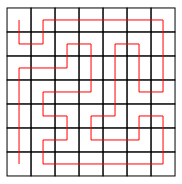
\includegraphics[scale=.5]{grid_path}
	\end{figure}
	\noindent corresponds to the description {\tt DRURRRRRDDDLUULDDDLDRRURDDLLLLLURULURRUULDLLDDDD}. You are given a description of a path which may also contain characters {\tt?} (any direction). Your task is to calculate the number of paths that match the description.
	\begin{itemize}
		\item {\sf Input.} The only input line has a $48$-character string of characters {\tt?, D, U, L, R}.
		\item {\sf Output.} Print 1 integer: the total number of paths.
		\item {\sf Sample.}
		\begin{table}[H]
			\centering
			\begin{tabular}{|l|l|}
				\hline
				\verb|grid_path.inp| & \verb|grid_path.out| \\
				\hline
				{\tt??????R??????U??????????????????????????LD????D?} & 201 \\
				\hline
			\end{tabular}
		\end{table}
	\end{itemize}
\end{problem}

%------------------------------------------------------------------------------%

\subsection{Mathematics}

\begin{problem}[Josephus Queries]
	Consider a game where there are $n$ children (numbered $1,2\ldots,n$) in a circle. During the game, every second child is removed from the circle, until there are no children left. Your task is to process $q$ queries of the form: ``when there are $n$ children, who is the $k$th child that will be removed?''	
	\begin{itemize}
		\item {\sf Input.} The 1st input line has a positive integer $q\in\mathbb{N}$: the number of queries. After this, there are $q$ lines that describe the queries. Each line has 2 integers $n,k\in\mathbb{N}$: the number of children \& the position of the child.
		\item {\sf Output.} Print $q$ integers: the answer for each query.
		\item {\sf Constraints.} $1\le q\le10^5$, $1\le k\le n\le10^9$.
		\item {\sf Sample.}
		\begin{table}[H]
			\centering
			\begin{tabular}{|l|l|}
				\hline
				\verb|Josephus_query.inp| & \verb|Josephus_query.out| \\
				\hline
				4 & 2 \\
				7 1 & 6 \\
				7 3 & 1 \\
				2 2 & 1107 \\
				1337 1313 & \\
				\hline
			\end{tabular}
		\end{table}
	\end{itemize}
\end{problem}

%------------------------------------------------------------------------------%

%------------------------------------------------------------------------------%

\section{Notes on Commands}

\subsection{Notes on C{\tt/}C++ commands}
Template:
\begin{Verbatim}[numbers=left,xleftmargin=5mm]
	#include <bits/stdc++.h>
	using namespace std;
	
	int main() {
		ios::sync_with_stdio(0);
		cin.tie(0);
		// Input & Output
		freopen("prob.inp", "r", stdin);
		freopen("prob.out", "w", stdout);	
	}
	// Terminal: g++ -std=c++11 -O2 -Wall test.cpp -o test
\end{Verbatim}

\subsection{Notes on Pascal commands}

\subsection{Notes on Python commands}

\begin{itemize}
	\item Để sử dụng các hàm toán học trong Python, cần import thư viện {\tt math} vào chương trình: {\tt from math import *}
	\item Để mở file dữ liệu vào {\tt prob.inp} chỉ để đọc dữ liệu \& mở file dữ liệu ra {\tt prob.out} để thay đổi dữ liệu trong file: {\tt file = open("prob.inp")} \& {\tt file2 = open("prob.out", "w")}.
	\item Sắp xếp trong Python có thể thực hiện 1 cách đơn giản nhờ phương thức {\tt sort()} hoặc {\tt sorted()}. Cú pháp:
	\begin{Verbatim}[numbers=left,xleftmargin=5mm]
		list.sort(reverse = True|False, key = myFunc)
		list.sorted(reverse = True|False, key = myFunc)
	\end{Verbatim}
	\item Trong Python, để lấy giá trị ngẫu nhiên, sử dụng phương thức {\tt ranint(a, b)} với {\tt a, b} là giới hạn của giá trị cần lấy ngẫu nhiên.
	\item Cf.: \texttt{**0.5} or \texttt{**(1/2)} vs. \texttt{math.sqrt(), cmath.sqrt()}:
	\begin{itemize}
		\item \href{https://www.learndatasci.com/solutions/python-square-root/}{Python Square Root: Real \& Complex -- Calculating the Square Root in Python}.\footnote{\url{https://www.learndatasci.com/solutions/python-square-root/}.}
		\item \href{https://stackoverflow.com/questions/327002/which-is-faster-in-python-x-5-or-math-sqrtx}{StackOverflow{\tt/}which is faster in Python: x**.5 or math.sqrt(x)?}.\footnote{\url{https://stackoverflow.com/questions/327002/which-is-faster-in-python-x-5-or-math-sqrtx}.}
	\end{itemize}
\end{itemize}

%------------------------------------------------------------------------------%

\section{Problems in Elementary Mathematics  -- Bài Toán Tin Học Trong Toán Học Sơ Cấp}

\begin{baitoan}[Even vs. odd]
	Viết thuật toán \& các chương trình bằng các ngôn ngữ lập trình {\sf Pascal, Python, C{\tt/}C++} để xét tính chẵn lẻ của $n\in\mathbb{Z}$ được nhập từ bàn phím.
\end{baitoan}
\noindent Pascal: \url{https://github.com/NQBH/hobby/blob/master/elementary_computer_science/Pascal/even_odd.pas}.
\begin{Verbatim}[numbers=left,xleftmargin=5mm]
	program even_odd;
	var n : integer;
	begin
	write('Enter n = '); readln(n);
	if n mod 2 = 0 then writeln(n,' is even') else writeln(n, ' is odd');
	end.
\end{Verbatim}
Python: \url{https://github.com/NQBH/hobby/blob/master/elementary_computer_science/Python/even_odd.py}
\begin{Verbatim}[numbers=left,xleftmargin=5mm]
	n = int(input())
	if n % 2 == 0:
	print(n, " is even")
	else:
	print(n, " is odd")
\end{Verbatim}
C: \url{https://github.com/NQBH/hobby/blob/master/elementary_computer_science/C/even_odd.c}.
\begin{Verbatim}[numbers=left,xleftmargin=5mm]
	#include <stdio.h>
	int main() {
		int n;
		scanf("%d", &n);
		// 1st solution
		if (n % 2 == 0) printf("%d is even.\n", n);
		else printf("%d is odd.\n", n);
		// 2nd solution
		(n % 2 == 0) ? printf("%d is even.\n", n) : printf("%d is odd.\n", n);
		// 3rd solution
		if ((n & 1) == 0) printf("%d is even.\n", n);
		else printf("%d is odd.\n", n);
		return 0;
	}
	// Terminal: g++ -std=c++11 -O2 -Wall even_odd.c -o even_odd
\end{Verbatim}
C++: \url{https://github.com/NQBH/hobby/blob/master/elementary_computer_science/Cpp/even_odd.cpp}.
\begin{Verbatim}[numbers=left,xleftmargin=5mm]
	#include <iostream>
	using namespace std;
	int main() {
		int n;
		cin >> n;
		// 1st solution
		if (n % 2 == 0) cout << n << " is even.\n";
		else cout << n << " is odd.\n";
		// 2nd solution
		(n % 2 == 0) ? cout << n << " is even.\n" : cout << n << " is odd.\n";
		// 3rd solution using bitwise AND
		if ((n & 1) == 0) cout << n << " is even.\n";
		else cout << n << " is odd.\n";
		return 0;
	}
	// Terminal: g++ -std=c++11 -O2 -Wall even_odd.cpp -o even_odd
\end{Verbatim}

\begin{baitoan}[Divisible by]
	Viết thuật toán \& các chương trình bằng các ngôn ngữ lập trình {\sf Pascal, Python, C{\tt/}C++} để kiểm tra liệu $a\divby b$ hay không, với $a,b\in\mathbb{Z}$ được nhập từ bàn phím \& in ra số dư $r$ trong phép chia $a$ cho $b$.
\end{baitoan}
\noindent Pascal: \url{{https://github.com/NQBH/hobby/blob/master/elementary_computer_science/Pascal/divisible_by.pas}}.
\begin{Verbatim}[numbers=left,xleftmargin=5mm]
	program divisible_by;
	var a, b : integer;
	begin
	write('Enter a = ');
	readln(a);
	write('Enter b = ');
	readln(b);
	if a mod b = 0 then writeln(a,' is divisible by ', b, '.')
	else writeln(a,' is not divisible by ', b, '.');
	end.
\end{Verbatim}
Python:
\begin{itemize}
	\item \url{https://github.com/NQBH/hobby/blob/master/elementary_computer_science/Python/divisible_by.py}.
	\item \url{https://github.com/NQBH/hobby/blob/master/elementary_computer_science/Python/HTP/divisible_by.py}.
\end{itemize} 
\begin{Verbatim}[numbers=left,xleftmargin=5mm]
	a = int(input())
	b = int(input())
	if a % b == 0:
	print(a, ' is divisible by ', b)
	else:
	print(a, ' is not divisible by ', b)
\end{Verbatim}
C: \url{https://github.com/NQBH/hobby/blob/master/elementary_computer_science/C/divisible_by.c}.
\begin{Verbatim}[numbers=left,xleftmargin=5mm]
	#include <stdio.h>
	int main() {
		int a, b;
		scanf("%d", &a);
		scanf("%d", &b);
		if (a % b == 0) printf("%d is divisible by %d.\n", a, b);
		else printf("%d is not divisible by %d.\n", a, b);
		return 0;
	}
	// Terminal: g++ -std=c++11 -O2 -Wall divisible_by.c -o divisible_by
\end{Verbatim}
C++: \url{https://github.com/NQBH/hobby/blob/master/elementary_computer_science/Cpp/divisible_by.cpp}.
\begin{Verbatim}[numbers=left,xleftmargin=5mm]
	#include <iostream>
	using namespace std;
	int main() {
		int a, b;
		cin >> a >> b;
		if (a % b == 0) cout << a << " is divisible by " << b << ".\n";
		else cout << a << " is not divisible by " << b << ".\n";
		return 0;
	}
	// Terminal: g++ -std=c++11 -O2 -Wall divisible_by.cpp -o divisible_by
\end{Verbatim}

\begin{baitoan}[Triangle]
	Viết thuật toán \& các chương trình bằng các ngôn ngữ lập trình {\sf Pascal, Python, C{\tt/}C++} để liệu $a,b,c$ có phải là độ dài của: (a) 1 tam giác. (b) 1 tam giác nhọn. (c) 1 tam giác vuông. (d) 1 tam giác tù.
\end{baitoan}
\noindent Pascal: 

\begin{itemize}
	\item Python script: \href{https://github.com/NQBH/hobby/blob/master/elementary_computer_science/Python/triangle.py}{GitHub{\tt/}NQBH{\tt/}hobby{\tt/}elementary computer science{\tt/}Python{\tt/}triangle}.
\end{itemize}

\begin{Verbatim}[numbers=left,xleftmargin=5mm]
	try:
	a,b,c = float(input('Nhap a = ')), float(input('Nhap b = ')), float(input('Nhap c = '))
	if (a + b > c) and (a + c > b) and  (b + c > a):
	loai_tg = ''
	if (a*a + b*b == c*c) or (a*a + c*c == b*b) or (b*b + c*c == a*a):
	loai_tg = 'vuong'
	elif (a*a + b*b > c*c) and (a*a + c*c > b*b) and (b*b + c*c > a*a):
	loai_tg = 'nhon'
	else:
	loai_tg = 'tu'
	print('Day la do dai 3 canh cua 1 tam giac ' + loai_tg)
	else: 
	print('Day khong la do dai 3 canh cua 1 tam giac.')			
	except:
	print('Day khong phai la 1 so.')
\end{Verbatim}

\begin{baitoan}[A special cubic equation -- 1 dạng phương trình bậc 3 đặc biệt]
	(a) Viết thuật toán \& các chương trình bằng các ngôn ngữ lập trình {\sf Pascal, Python, C{\tt/}C++} để giải phương trình bậc 3 có dạng đặc biệt $x^3 + 3a^2x + 2b = 0$ (khuyết số hạng $x^2$), với $p,q\in\mathbb{R}$ được nhập từ bàn phím. Biết phương trình này có 1 nghiệm duy nhất là\footnote{See. e.g., \cite[pp. 68--69]{Thu_Phuong_Tien_Triet_NMLT}.}:
	\begin{align*}
		x = \sqrt[3]{\sqrt{a^6 + b^2} - b} - \sqrt[3]{\sqrt{a^6 + b^2} + b}.
	\end{align*}
	(b) Chứng minh chặt chẽ bằng toán học công thức nghiệm đã cho.
\end{baitoan}
C: \url{https://github.com/NQBH/hobby/blob/master/elementary_computer_science/C/special_cubic_eqn.c}.
\begin{Verbatim}[numbers=left,xleftmargin=5mm]
	#include <math.h>
	#include <stdio.h>
	int main() {
		double a, b, x, delta, test;
		printf("a = ");
		scanf("%lf", &a);
		printf("b = ");
		scanf("%lf", &b);
		delta = pow(a, 6.0) + pow(b, 2.0);
		delta = sqrt(delta);
		x = pow(delta - b, 1.0/3) - pow(delta + b, 1.0/3);
		printf("Root x = %lf.\n", x);
		test = x*x*x + 3*a*a*x + 2*b;
		printf("x^3 + 3a^2x + 2b = %lf.\n", test);
	}
\end{Verbatim}
C++: \url{https://github.com/NQBH/hobby/blob/master/elementary_computer_science/Cpp/special_cubic_eqn.cpp}.
\begin{Verbatim}[numbers=left,xleftmargin=5mm]
	#include <cmath>
	#include <iostream>
	using namespace std;
	int main() {
		double a, b, x, delta;
		cout << "a = ";
		cin >> a;
		cout << "b = ";
		cin >> b;
		delta = pow(a, 6.0) + pow(b, 2.0);
		delta = sqrt(delta);
		x = pow(delta - b, 1.0/3) - pow(delta + b, 1.0/3);
		cout << "Root x = " << x << ".\n";
		double test = x*x*x + 3*a*a*x + 2*b;
		cout << "x^3 + 3a^2x + 2b = " << test << ".\n";
	}
\end{Verbatim}

\begin{baitoan}[Polynomial equation -- Phương trình đa thức]
	Viết thuật toán \& các chương trình bằng các ngôn ngữ lập trình {\sf Pascal, Python, C{\tt/}C++} để giải phương trình bậc nhất, bậc 2, bậc 3, \& bậc 4 với các hệ số thực được nhập từ bàn phím.
\end{baitoan}

\begin{baitoan}[Fibonacci sequence]
	Viết thuật toán \& các chương trình bằng các ngôn ngữ lập trình {\sf Pascal, Python, C{\tt/}C++} để xuất ra màn hình, với $n\in\mathbb{N}$ được nhập từ bàn phím: (a) Số Fibonacci thứ $n$. (b) $n$ số Fibonacci đầu tiên.
\end{baitoan}

\begin{baitoan}[1st $n$ square roots]
	Viết chương trình {\sf Pascal, C{\tt/}C++, Python} xuất ra căn bậc 2 của $n$ số tự nhiên đầu tiên với $n\in\mathbb{N}^\star$ được nhập từ bàn phím.
\end{baitoan}

\begin{baitoan}[Số chính phương -- Square number]
	Viết chương trình {\sf Pascal, C{\tt/}C++, Python} để kiểm tra 1 số $n\in\mathbb{N}^\star$ được nhập từ bàn phím có phải là số chính phương hay không.
\end{baitoan}

\begin{baitoan}[1st $n$ cube roots]
	Viết chương trình {\sf Pascal, C{\tt/}C++, Python} xuất ra căn bậc 3 của $n$ số tự nhiên đầu tiên với $n\in\mathbb{N}^\star$ được nhập từ bàn phím.
\end{baitoan}

\begin{baitoan}
	Viết chương trình {\sf Pascal, C{\tt/}C++, Python} để kiểm tra 1 số $n\in\mathbb{N}^\star$ được nhập từ bàn phím có phải là lập phương của 1 số tự nhiên hay không.
\end{baitoan}

\begin{baitoan}[1st $n$ $n$th roots]
	Viết chương trình {\sf Pascal, C{\tt/}C++, Python} xuất ra căn bậc $n$ của $m$ số tự nhiên đầu tiên với $m,n\in\mathbb{N}^\star$ được nhập từ bàn phím.
\end{baitoan}

\begin{baitoan}
	Viết chương trình {\sf Pascal, C{\tt/}C++, Python} để kiểm tra 1 số $m\in\mathbb{Z}$ được nhập từ bàn phím có phải là lũy thừa bậc $n\in\mathbb{N}$ của 1 số tự nhiên hay không với $m,n$ được nhập từ bàn phím.
\end{baitoan}

\begin{baitoan}[\cite{Duc_200_BT_Python}, 1., p. 18, Thay chữ số -- Digit replacement]
	Lập trình vào số nguyên $n\in\mathbb{Z}$, thực hiện thay thế các chữ số $0$ trong biểu diễn thập phân của $n$ thành các chữ số $5$ \& in ra kết quả.
	\begin{itemize}
		\item {\sf Input.} Dòng đầu tiên của đầu vào chứa số nguyên $T$ cho biết số bộ dữ liệu cần kiểm tra. Mỗi bộ dữ liệu gồm 1 dòng chứa 1 số nguyên $n\in\mathbb{Z}$.
		\item {\sf Output.} Ứng với mỗi bộ dữ liệu đầu vào, chương trình cần in ra số $n$ sau khi thay thế các chữ số của $n$ theo yêu cầu đề bài.
		\item {\sf Constraint.} $1\le T\le10^5$, $0\le n\le10^{12}$.
		\item {\sf Sample.}
		\begin{table}[H]
			\centering
			\begin{tabular}{|l|l|}
				\hline
				\verb|digit_replacement.inp| & \verb|digit_replacement.out| \\
				\hline
				2 & 1555 \\
				1005 & 1234 \\
				1234 &  \\
				\hline
			\end{tabular}
		\end{table}
	\end{itemize}
\end{baitoan}
Python:
\begin{itemize}
	\item {\small\url{https://github.com/NQBH/hobby/blob/master/elementary_computer_science/Python/Duc_200_BTLT_Python/digit_replacement.py}}.
	\item \url{https://github.com/NQBH/hobby/blob/master/elementary_computer_science/Python/digit_replacement.py}.
	\item \url{https://github.com/NQBH/hobby/blob/master/elementary_computer_science/Python/HTP/digit_replacement.py}.
	\item Input: \url{https://github.com/NQBH/hobby/blob/master/elementary_computer_science/Python/digit_replacement.inp}.
	\item Output: \url{https://github.com/NQBH/hobby/blob/master/elementary_computer_science/Python/digit_replacement.out}.
\end{itemize}
\begin{multicols}{2}
	1st solution \cite[1., p. 202]{Duc_200_BT_Python}:
	\begin{Verbatim}[numbers=left,xleftmargin=5mm]
		def convert5(n):
		if n == 0:
		return 5
		y = [c for c in n]
		for i in range(len(y)):
		if y[i] == '0':
		y[i] = '5'
		return ''.join(y)
		t = int(input())
		while t != 0:
		t -= 1
		n = input()
		print(convert5(n))
	\end{Verbatim}
	\columnbreak
	2nd solution:
	\begin{Verbatim}[numbers=left,xleftmargin=5mm]
		def digit_replacement(n):
		ans = ''
		for i in range(len(n)):
		if n[i] == '0':
		ans += '5'
		else:
		ans += n[i]
		return ans
		t = int(input())
		for _ in range(t):
		n = input()
		print(digit_replacement(n))
	\end{Verbatim}
\end{multicols}
3rd solution:
\begin{Verbatim}[numbers=left,xleftmargin=5mm]
	t = int(input())
	A = []
	for _ in range(t):
	s = input()
	A += [s.replace('0', '5')]
	print('\n'.join(A))
\end{Verbatim}

\begin{nhanxet}
	Bài toán trên có thể mở rộng cho việc thay chữ số $0$ thành $5$ thành việc thay chữ số $a$ thành chữ số $b$ với $a,b\in\{0,1,2,\ldots,9\}$ là các chữ số bất kỳ, chỉ cần đổi các dòng lệnh tương ứng thành:
	\begin{multicols}{3}
		\begin{verbatim}
			if n[i] == '<a>':
			ans += '<b>'
		\end{verbatim}
		\begin{verbatim}
			if n[i] == '<a>':
			ans += '<b>'
		\end{verbatim}
		\verb|A += [s.replace('<a>', '<b>')]|
	\end{multicols}
	\noindent trong đó \verb|<a>, <b>| lần lượt là 2 giá trị của cặp chữ số cần đổi thành: $a\to b$. Tương tự, có thể thay 1 bộ nhiều chữ số thành 1 bộ chữ số khác, i.e., $(a_1,a_2,\ldots,a_n)\to(b_1,b_2,\ldots,b_n)$, với $n\in\mathbb{N}$, $a_i,b_i\in\{0,1,2,\ldots,9\}$, $\forall i = 1,2,\ldots,n$ thay vì chỉ 1 chữ số.
\end{nhanxet}

\begin{baitoan}[\cite{Duc_200_BT_Python}, 2., pp. 18--19, Dice -- Xúc xắc]
	Bạn được tặng 1 con xúc xắc hình lập phương với $6$ mặt. Mỗi mặt của con xúc xắc có in 1 số chấm, số lượng chấm $\in\{1,2,3,4,5,6\}$. Bạn được biết số chấm trên 1 mặt của xúc xắc, nhiệm vụ là đoán số ở mặt đối diện của xúc xắc.
	\begin{itemize}
		\item {\sf Input.} Dòng đầu tiên của đầu vào chứa số nguyên dương $t\in\mathbb{N}^\star$ cho biết số bộ dữ liệu cần kiểm tra. Mỗi bộ dữ liệu gồm 1 dòng chứa 1 số nguyên $n\in\mathbb{Z}$ cho biết số chấm trên 1 mặt của con xúc xắc.
		\item {\sf Output.} Ứng với mỗi bộ dữ liệu đầu vào, in ra số ở mặt đối diện tương ứng.
		\item {\sf Constraint.} $1\le t\le500$, $1\le n\le6$.
		\item {\sf Sample.}
		\begin{table}[H]
			\centering
			\begin{tabular}{|l|l|}
				\hline
				{\tt dice.inp} & {\tt dice.out} \\
				\hline
				2 & 1 \\
				6 & 5 \\
				2 &  \\
				\hline
			\end{tabular}
		\end{table}
	\end{itemize}
\end{baitoan}
Tổng số chấm trên 2 mặt đối nhau của 1 con xúc xắc luôn bằng 7, nên đối diện với mặt có số chấm là $n\in\{1,2,3,4,5,6\}$ là mặt có số chấm $7 - n\in\{1,2,3,4,5,6\}$.

Pascal:

Python:
\begin{itemize}
	\item \url{https://github.com/NQBH/hobby/blob/master/elementary_computer_science/Python/dice.py}.
	\item \url{https://github.com/NQBH/hobby/blob/master/elementary_computer_science/Python/Duc_200_BTLT_Python/dice.py}.
	\item \url{https://github.com/NQBH/hobby/blob/master/elementary_computer_science/Python/HTP/dice.py}.
	\item Input: \url{https://github.com/NQBH/hobby/blob/master/elementary_computer_science/Python/dice.inp}.
	\item Output: \url{https://github.com/NQBH/hobby/blob/master/elementary_computer_science/Python/dice.out}.
\end{itemize}
\begin{multicols}{2}
	1st solution \cite[p. 202--203]{Duc_200_BT_Python}:
	\begin{Verbatim}[numbers=left,xleftmargin=5mm]
		t = int(input())
		while t != 0:
		t -= 1
		n = int(input())
		print(7 - n)
	\end{Verbatim}
	\columnbreak
	2nd solution:
	\begin{Verbatim}[numbers=left,xleftmargin=5mm]
		t = int(input())
		for _ in range(t):
		n = int(input())
		print(7 - n)
	\end{Verbatim}
\end{multicols}

\begin{baitoan}[\cite{Duc_200_BT_Python}, 3., pp. 19--20, Doctor appointment -- Lịch khám bệnh]
	Có $n\in\mathbb{N}^\star$ bệnh nhân đến khám bệnh tại phòng khám. Giả sử cứ sau $x$ phút thì lại có 1 bệnh nhân mới đến phòng khám. Ngoài ra, bác sĩ sẽ chỉ dành $10$ phút để khám cho mỗi bệnh nhân. Tính toán thời gian bằng phút mà bệnh nhân cuối cùng cần phải chờ đến lượt mình được bác sĩ khám bệnh.
	\begin{itemize}
		\item {\sf Input.} Dòng đầu tiên của đầu vào chứa số nguyên dương $t\in\mathbb{N}^\star$ cho biết số bộ dữ liệu cần kiểm tra. Mỗi bộ dữ liệu gồm 1 dòng chứa 2 số nguyên $n,x\in\mathbb{Z}$.
		\item {\sf Output.} Ứng với mỗi bộ dữ liệu đầu vào, in ra 1 dòng chứa số $m$ là số phút mà bệnh nhân cuối cùng cần chờ bác sĩ tại phòng khám.
		\item {\sf Constraint.} $1\le t\le500$, $1\le n\le100$, $0\le x\le30$.
		\item {\sf Sample.}
		\begin{table}[H]
			\centering
			\begin{tabular}{|l|l|}
				\hline
				\verb|doctor_appointment.inp| & \verb|doctor_appointment.out| \\
				\hline
				5 & 15 \\
				4 5 & 28 \\
				5 3 & 25 \\
				6 5 & 24 \\
				7 6 & 56 \\
				8 2 & \\
				\hline
			\end{tabular}
		\end{table}
	\end{itemize}
\end{baitoan}
\noindent Python: \url{https://github.com/NQBH/hobby/blob/master/elementary_computer_science/Python/doctor_appointment.py}.
\begin{multicols}{2}
	1st solution \cite[3., p. 203]{Duc_200_BT_Python}
	\begin{Verbatim}[numbers=left,xleftmargin=5mm]
		t = int(input())
		while t != 0:
		t -= 1
		n, x = map(int, input().split())
		ans = x + 10*(n - 1) - x*n
		if ans < 0:
		ans = 0
		print(ans)
	\end{Verbatim}
	\columnbreak
	2nd solution:
	\begin{Verbatim}[numbers=left,xleftmargin=5mm]
		t = int(input())
		while t != 0:
		t -= 1
		n, x = map(int, input().split())
		if x >= 10:
		print(0)
		else:
		print((n - 1)*(10 - x))
	\end{Verbatim}
\end{multicols}

\begin{baitoan}[\cite{Duc_200_BT_Python}, 4., p. 20, Bit even, bit odd -- Tính chẵn lẻ nhị phân]
	Cho số nguyên không dấu $n\in\mathbb{N}$. Kiểm tra ``tính chẵn lẻ'' của $n$, với \emph{tính chẵn lẻ} của $n$ là số bit {\tt1} trong biểu diễn nhị phân của $n$, i.e., nếu trong biểu diễn nhị phân của $n$ có chứa 1 số chẵn các bit {\tt1} thì $n$ được coi là có tính chẵn, \& ngược lại $n$ có tính lẻ.
	\begin{itemize}
		\item {\sf Input.} Dòng đầu tiên của đầu vào chứa số nguyên dương $t\in\mathbb{N}^\star$ cho biết số bộ dữ liệu cần kiểm tra. Mỗi bộ dữ liệu gồm 1 dòng chứa số nguyên $n\in\mathbb{N}$.
		\item {\sf Output.} Ứng với mỗi bộ dữ liệu đầu vào, in ra 1 dòng chứa thông báo {\tt"odd"} nếu $n$ có tính lẻ \& {\tt"even"} nếu $n$ có tính chẵn.
		\item {\sf Constraint.} $1\le t\le500$, $1\le n\le10^{12}$.
		\item {\sf Sample.}
		\begin{table}[H]
			\centering
			\begin{tabular}{|l|l|}
				\hline
				\verb|bit_even_odd.inp| & \verb|bit_even_odd.out| \\
				\hline
				2 & odd \\
				13 & even \\
				9 & \\
				\hline
			\end{tabular}
		\end{table}
	\end{itemize}
\end{baitoan}
Đổi $n$ sang biểu diễn nhị phân, đếm các số 1.

\noindent Python: \url{https://github.com/NQBH/hobby/blob/master/elementary_computer_science/Python/bit_even_odd.py}.
\begin{multicols}{2}
	1st solution \cite[4., p. 204]{Duc_200_BT_Python}:
	\begin{Verbatim}[numbers=left,xleftmargin=5mm]
		t = int(input())
		while t != 0:
		t -= 1
		s = 0
		n = int(input())
		while n != 0:
		s += n % 2
		n //= 2
		if s % 2 != 0:
		print("odd")
		else:
		print("even")
	\end{Verbatim}
	\columnbreak
	2nd solution:
	\begin{Verbatim}[numbers=left,xleftmargin=5mm]
		t = int(input())
		while t != 0:
		t -= 1
		s = 0
		n = bin(int(input()))
		for c in n:
		if c == '1':
		s += 1
		if s % 2 != 0:
		print("odd")
		else:
		print("even")
	\end{Verbatim}
\end{multicols}

\begin{baitoan}[\cite{Duc_200_BT_Python}, 5., pp. 20--21, Message -- Nhắn tin]
	Có $n\in\mathbb{N}^\star$ học sinh trong 1 lớp học, mỗi người nghĩ ra 1 câu chuyện hài hước khác nhau. Trong 1 giờ vắng giáo viên, họ quyết định nghĩa ra 1 trò chơi để giết thời gian. Họ muốn chia sẻ những câu chuyện hài hước với nhau bằng cách gửi tin nhắn điện tử. Giả sử 1 người luôn gửi tất cả những câu chuyện hài hước mà người ấy biết tại thời điểm tin nhắn được gửi \& 1 tin nhắn chỉ có thể gửi đến 1 người nhận. Số lượng tin nhắn tối thiểu họ cần gửi là bao nhiêu để đảm bảo tất cả $n$ người đều nhận được tất cả các câu chuyện?
	\begin{itemize}
		\item {\sf Input.} Dòng đầu tiên của đầu vào chứa số nguyên dương $t\in\mathbb{N}^\star$ cho biết số bộ dữ liệu cần kiểm tra. Mỗi bộ dữ liệu gồm 1 dòng chứa số nguyên $n\in\mathbb{N}$.
		\item {\sf Output.} Ứng với mỗi bộ dữ liệu đầu vào, in ra 1 dòng chứa số lượng tin nhắn cần gửi để $n$ học sinh đều nhận được tất cả $n$ câu chuyện hài.
		\item {\sf Constraint.} $1\le t\le100$, $1\le n\le10^5$.
		\item {\sf Sample.}
		\begin{table}[H]
			\centering
			\begin{tabular}{|l|l|}
				\hline
				{\tt message.inp} & {\tt message.out} \\
				\hline
				1 & 2 \\
				2 & \\
				\hline
			\end{tabular}
		\end{table}
	\end{itemize}
\end{baitoan}
\noindent Pascal:

Python: \url{https://github.com/NQBH/hobby/blob/master/elementary_computer_science/Python/message.py}.
\begin{Verbatim}[numbers=left,xleftmargin=5mm]
	t = int(input())
	for _ in range(t):
	n = int(input())
	print(2*n - 2)
\end{Verbatim}
C++:
\begin{itemize}
	\item \url{https://github.com/NQBH/hobby/blob/master/elementary_computer_science/Cpp/message.cpp}.
	\item \url{https://github.com/NQBH/hobby/blob/master/elementary_computer_science/Cpp/HTP/message.cpp}.
	\item Input: \url{https://github.com/NQBH/hobby/blob/master/elementary_computer_science/Cpp/message.inp}.
	\item Output: \url{https://github.com/NQBH/hobby/blob/master/elementary_computer_science/Cpp/message.out}.
\end{itemize}

\begin{multicols}{2}
	1st solution:
	\begin{Verbatim}[numbers=left,xleftmargin=5mm]
		#include <iostream>
		using namespace std;
		
		int main() {
			int t, n;
			cin >> t;
			int A[t];
			for (int i = 0; i < t; ++i) {
				cin >> n;
				A[i] = n*(n - 1);
				cout << A[i] << '\n';
			}
		}	
	\end{Verbatim}
	\columnbreak
	2nd solution:
	\begin{Verbatim}[numbers=left,xleftmargin=5mm]
		#include <iostream>
		using namespace std;
		
		int main() {
			int t, n;
			cin >> t;
			while (t--) {
				cin >> n;
				cout << 2*n - 2 << '\n';
			}
		}
	\end{Verbatim}
\end{multicols}

\begin{baitoan}[\cite{Duc_200_BT_Python}, 6., pp. 21--22, Triangle number -- Số tam giác]
	1 số được gọi là \emph{số tam giác} nếu ta có thể biểu diễn nó dưới dạng lưới hình tam giác gồm các điểm sao cho các điểm tạo thành 1 tam giác đều, i.e., hàng đầu tiên có $1$ điểm, hàng thứ 2 có $2$ điểm, $\ldots$ hàng thứ $i$ có $i$ điểm. Các số tam giác đầu tiên là $1$, $3 = 1 + 2$, $6 = 1 + 2 + 3$, $10 = 1 + 2 + 3 + 4$. Cho số nguyên dương $n\in\mathbb{N}^\star$, kiểm tra xem $N$ có phải là số tam giác hay không. 
	\begin{itemize}
		\item {\sf Input.} Dòng đầu tiên của đầu vào chứa số nguyên dương $t\in\mathbb{N}^\star$ cho biết số bộ dữ liệu cần kiểm tra. Mỗi bộ dữ liệu gồm 1 dòng chứa số nguyên $n\in\mathbb{N}$.
		\item {\sf Output.} Ứng với mỗi bộ dữ liệu đầu vào, in ra 1 dòng chứa số $1$ nếu $n$ là số tam giác, ngược lại thì in ra số $0$.
		\item {\sf Constraint.} $1\le t\le100$, $1\le n\le10^7$.
		\item {\sf Sample.}
		\begin{table}[H]
			\centering
			\begin{tabular}{|l|l|}
				\hline
				\verb|triangle_number.inp| & \verb|triangle_number.out| \\
				\hline
				5 & 1 \\
				3 & 0 \\
				4 & 1 \\
				6 & 1 \\
				55 & 0 \\
				345 & \\
				\hline
			\end{tabular}
		\end{table}
	\end{itemize}
\end{baitoan}
See, e.g., \href{https://vi.wikipedia.org/wiki/S%E1%BB%91_tam_gi%C3%A1c}{Wikipedia{\tt/}số tam giác} or \href{https://en.wikipedia.org/wiki/Triangular_number}{Wikipedia{\tt/}triangular number}.

Python:
\begin{itemize}
	\item \url{https://github.com/NQBH/hobby/blob/master/elementary_computer_science/Python/Duc_200_BTLT_Python/triangle_number.py}.
	\item \url{https://github.com/NQBH/hobby/blob/master/elementary_computer_science/Python/triangle_number.py}.
	\item \url{https://github.com/NQBH/hobby/blob/master/elementary_computer_science/Python/HTP/triangle_number.py}.
	\item Input: \url{https://github.com/NQBH/hobby/blob/master/elementary_computer_science/Python/triangle_number.inp}.
	\item Output: \url{https://github.com/NQBH/hobby/blob/master/elementary_computer_science/Python/triangle_number.out}.
\end{itemize}

\begin{multicols}{2}
	1st solution \cite[6., pp. 204--205]{Duc_200_BT_Python}:
	\begin{Verbatim}[numbers=left,xleftmargin=5mm]
		from math import sqrt, floor
		t = int(input())
		for _ in range(t):
		n = int(input())
		a, b = 1, 1
		c = -2*n
		d = b*b - 4*a*c
		x1 = (-b + sqrt(d))/(2*a)
		x2 = (-b - sqrt(d))/(2*a)
		if x1 > 0 and floor(x1) == x1:
		print('1')
		continue
		if x2 > 0 and floor(x2) == x2:
		print('1')
		continue
		print('0')
	\end{Verbatim}
	\columnbreak
	2nd solution:
	\begin{Verbatim}[numbers=left,xleftmargin=5mm]
		t = int(input())
		for _ in range(t):
		n = int(input())
		i = 1
		sum = 0
		while sum < n:
		sum += i
		i += 1
		if n == sum:
		print(1)
		else:
		print(0)
	\end{Verbatim}
\end{multicols}

\begin{multicols}{2}
	3rd solution:
	\begin{Verbatim}[numbers=left,xleftmargin=5mm]
		from math import sqrt
		def is_triangle_number(x):
		x = x*8 + 1
		if int(sqrt(x))**2 != x:
		return 0
		return int(sqrt(x)) % 2
		t = int(input())
		A = []
		for _ in range(t):
		n = int(input())
		A += [str(is_triangle_number(n))]
		print('\n'.join(A))
	\end{Verbatim}
	\columnbreak
	4th solution:
	\begin{Verbatim}[numbers=left,xleftmargin=5mm]
		from math import sqrt, floor
		t = int(input())
		for _ in range(t):
		n = int(input())
		k = floor(sqrt(2*n))
		if n == k*(k + 1)/2:
		print(1)
		else:
		print(0)
	\end{Verbatim}
\end{multicols}

\begin{baitoan}
	Cho $n\in\mathbb{N}^\star$ nhập từ bàn phím. (a) In số tam giác thứ $n$. (b) In $n$ số tam giác đầu tiên. (c) Cho $a,b\in\mathbb{R}$ nhập từ bàn phím, in tất cả các số tam giác thuộc đoạn $[a,b]$.
\end{baitoan}


%------------------------------------------------------------------------------%

\subsection{Algebraic Expression -- Biểu Thức Đại Số}

\begin{baitoan}[\cite{VietSTEM2021}, 1., p. 15, Vũng Tàu 2020]
	Cho $a,b,c\in\mathbb{N}^\star$. {\sf Yêu cầu:} Tính giá trị của biểu thức $S = \dfrac{a^2 + b^2 + c^2}{abc} + \sqrt{abc}$.
	\begin{itemize}
		\item {\sf Input.} File \verb|algebraic_expression.inp| chứa 3 số nguyên dương $a,b,c$. Mỗi số trên 1 dòng.
		\item {\sf Kết quả:} Ghi vào File \verb|algebraic_expression.out| kết quả $S$ tính được (làm tròn lấy 2 chữ số sau phần thập phân). E.g.:
		\begin{table}[H]
			\centering
			\begin{tabular}{|l|l|}
				\hline
				\verb|algebraic_expression.inp| & \verb|algebraic_expression.out| \\
				\hline
				2 & 4.25 \\
				1 &  \\
				2 &  \\
				\hline
			\end{tabular}
		\end{table}
	\end{itemize}
\end{baitoan}
Python script:
\begin{itemize}
	\item \url{https://github.com/NQBH/hobby/blob/master/elementary_computer_science/Python/algebraic_expression.py}.
\end{itemize}
Python:
\begin{Verbatim}[numbers=left,xleftmargin=5mm]
	from math import sqrt
	def algebraic_expression(a, b, c):
	return (a**2 + b**2 + c**2)/(a*b*c) + sqrt(a*b*c) # function f(a,b,c) can be modified
	a = int(input())
	b = int(input())
	c = int(input())
	print(algebraic_expression(a,b,c))
\end{Verbatim}
C:
\begin{itemize}
	\item \url{https://github.com/NQBH/hobby/blob/master/elementary_computer_science/C/algebraic_expression.c}.
	
	See also C-code for $f(x,y) = x + \sqrt{1 + y^2}$:
	\item \url{https://github.com/NQBH/hobby/blob/master/elementary_computer_science/C/sqrt_algebraic_expression.c}.
\end{itemize}

\begin{Verbatim}[numbers=left,xleftmargin=5mm]
	#include <math.h>
	#include <stdio.h>
	int main() {
		double a, b, c;
		scanf("%lf %lf %lf", &a, &b, &c);
		printf("%.2f.\n", (a*a + b*b + c*c)/(a*b*c) + sqrt(a*b*c));
		return 1;
	}
\end{Verbatim}
C++:
\begin{itemize}
	\item \url{https://github.com/NQBH/hobby/blob/master/elementary_computer_science/Cpp/algebraic_expression.cpp}.
	
	See also C-code for $f(x,y) = x + \sqrt{1 + y^2}$:
	\item \url{https://github.com/NQBH/hobby/blob/master/elementary_computer_science/Cpp/sqrt_algebraic_expression.cpp}.
\end{itemize}
\begin{Verbatim}[numbers=left,xleftmargin=5mm]
	#include <cmath>
	#include <iostream>
	using namespace std;
	int main() {
		double a, b, c;
		cin >> a >> b >> c;
		printf("%.2f\n", (a*a + b*b + c*c)/(a*b*c) + sqrt(a*b*c));
		return 1;
	}
\end{Verbatim}

\begin{luuy}
	Tương tự, ta có thể tính hầu như bất kỳ hàm số $f(a,b,c)$ 3 biến $a,b,c$ với $f$ là 1 hàm số có thể viết được nhờ thư viện {\tt math} của Python. Tổng quát hơn, ta có thể tính bất kỳ hàm số nhiều biến $f(x_1,x_2,\ldots,x_n)$ với $x_i$, $i = 1,2,\ldots,n$, $n\in\mathbb{N}^\star$ là các biến, với $f$ là 1 hàm số có thể viết được nhờ thư viện {\tt math} của Python.
\end{luuy}

\begin{baitoan}[\cite{VietSTEM2021}, 2., p. 19, Bắc Giang 2020]
	Nhà An có 1 trang trại rộng lớn. Do sở thích của An nên bố An chỉ nuôi gà \& chó. 1 hôm bố An đố con gái nhà mình nuôi bao nhiêu gà, bao nhiêu chó? Bố An cho biết nhà có tổng số gà \& chó là $x$ con. Do số lượng nhiều \& khó đếm từng loại nên An chỉ đếm được tổng số chân của gà \& chó là $y$ chân. Giúp An trả lời câu đố.
	\begin{itemize}
		\item {\sf Input.} Đọc từ file văn bản \verb|toanco.inp| gồm 2 số nguyên dương $x,y$ trên 1 dòng. 2 số cách nhau 1 khoảng trống ($x\le10^5$, $y\le4\cdot10^5$).
		\item {\sf Kết quả:} Ghi ra file văn bản \verb|toanco.out| gồm 2 số tương ứng là số gà \& số chó tìm được. 2 số cách nhau 1 khoảng trống. Giả sử bài toán luôn có nghiệm.
		\begin{table}[H]
			\centering
			\begin{tabular}{|l|l|}
				\hline
				{\tt toanco.inp} & {\tt toanco.out} \\
				\hline
				36 100 & 22 14 \\
				\hline
			\end{tabular}
		\end{table}
	\end{itemize}
\end{baitoan}
Python script: \href{https://github.com/NQBH/hobby/blob/master/elementary_computer_science/Python/toanco.py}{GitHub{\tt/}NQBH{\tt/}hobby{\tt/}elementary computer science{\tt/}Python{\tt/}toanco.py}\footnote{\textsc{url}: \url{https://github.com/NQBH/hobby/blob/master/elementary_computer_science/Python/toanco.py}.}. Input: \href{https://github.com/NQBH/hobby/blob/master/elementary_computer_science/Python/toanco.inp}{toanco.inp}. Output: \href{https://github.com/NQBH/hobby/blob/master/elementary_computer_science/Python/toanco.out}{toanco.out}.
\begin{Verbatim}[numbers=left,xleftmargin=5mm]
	file_in = open("toanco.inp")
	file_out = open("toanco.out", "w")
	s = file_in.readline()
	s = s.split()
	x = int(s[0])
	y = int(s[1])
	a = int(2*x - y/2)
	b = int(y/2 - x)
	file_out.write(str(a) + " " + str(b))
	file_in.close()
	file_out.close()
\end{Verbatim}

\begin{baitoan}[\cite{VietSTEM2021}, 4., p. 26, Quãng Ngãi 2020, Lãi suất-- Interest rate]
	1 người gửi tiền vào ngân hàng có kỳ hạn là $c$ tháng với lãi suất mỗi tháng là $k$\emph{\%}, số tiền gửi ban đầu là $A$ (đơn vị triệu đồng). 
	\begin{itemize}
		\item {\sf Yêu cầu:} Tính số tiền người đó nhận được sau $t$ tháng. Biết tiền lãi mỗi tháng được cộng dồn vào tiền gốc, nếu nhận tiền trước kỳ hạn thì số tiền được tính với lãi suất không kỳ hạn là $h$\emph{\%} của số tiền ban đầu $A$ nhân với số tháng đã gửi. Trong trường hợp rút tiền sau kỳ hạn thì số tháng sau kỳ hạn sẽ được tính với lãi suất không kỳ hạn là $h$\emph{\%} so với số tiền thu được đã qua kỳ hạn.
		\item {\sf Input.} Tệp văn bản \verb|bl2.inp| ghi $5$ số kỳ hạn $c$ (nếu $c = 0$ là gửi không kỳ hạn), thời gian gửi $t$, số tiền ban đầu $A$, lãi suất có kỳ hạn $k$, lãi suất không kỳ hạn $h$, các số cách nhau 1 ký tự trắng.
		\item {\sf Output.} Tệp văn bản \verb|bl2.out| ghi $1$ số là số tiền nhận được (làm tròn đến $1$ số lẻ sau dấu chấm thập phân). E.g.:
		\begin{table}[H]
			\centering
			\begin{tabular}{|l|l|}
				\hline
				{\tt bl2.inp} & {\tt bl2.out} \\
				\hline
				12 13 100 1.0 0.2 & 112.9 \\
				\hline
				0 10 100 1.0 0.2 & 102.0 \\
				\hline
			\end{tabular}
		\end{table}
	\end{itemize}
\end{baitoan}

%------------------------------------------------------------------------------%

\subsection{Number Theory -- Số Học}

\begin{baitoan}[\cite{VietSTEM2021}, 3., p. 20, Yên Bái 2020, Tổng nguyên tố]
	Viết chương trình nhập vào $2$ số nguyên $a,b\in\mathbb{Z}$, $0 < a < b$. (a) Tìm \& tính tổng các số nguyên tố của dãy số từ $a$ đến $b$. (b) Xuất ra màn hình các số chia hết cho $5$ của dãy số từ $a$ đến $b$. (c) \emph{(Bội của $n\in\mathbb{N}^\star$)} Xuất ra màn hình các số chia hết cho $n$ của dãy số từ $a$ đến $b$ với $n\in\mathbb{N}^\star$ được nhập từ bàn phím. E.g., nhập $a = 6$, $b = 22$. Kết quả tổng các số nguyên tố trong dãy số từ $6$ đến $22$: $7 + 11 + 13 + 17 + 19 = 67$. Các số chia hết cho $5$ của dãy số từ $6$ đến $22$: $10,15,20$.
\end{baitoan}

\begin{baitoan}[\cite{VietSTEM2021}, 4., p. 22, Hải Dương 2020, Số mạnh mẽ]
	\emph{Số mạnh mẽ} là số khi nó chia hết cho 1 số nguyên tố thì cũng chia hết cho cả bình phương của số nguyên tố đó, i.e., $a\in\mathbb{N}^\star$ là số mạnh mẽ $\Leftrightarrow$ ($a\divby p\Rightarrow a\divby p^2$, $\forall p$: prime). E.g., $25$ là số mạnh mẽ, vì nó chia hết cho số nguyên tố $5$ \& chia hết cho cả $5^2 = 25$. Viết chương trình liệt kê các số mạnh mẽ không vượt quá $1000$.
\end{baitoan}
See, e.g., \href{https://en.wikipedia.org/wiki/Powerful_number}{Wikipedia{\tt/}powerful number}, \href{https://mathworld.wolfram.com/PowerfulNumber.html}{MathWorld{\tt/}powerful number}.

\begin{baitoan}[\cite{VietSTEM2021}, 5., p. 23, Việt Nam 2020, Bội chính phương]
	Cho 1 dãy số $A$ có $n$ phần tử. Tìm số nguyên dương $a$ nhỏ nhất thỏa mãn: $a$ là số chính phương \& $a$ chia hết cho tất cả các phần tử của dãy số $A$.
	\begin{itemize}
		\item {\sf Yêu cầu:} In ra phần dư của phép chia khi chia $a$ cho $10^9 + 7$.
		\item {\sf Input.} Vào từ thiết bị theo khuôn dạng sau: Dòng đầu tiên chứa số nguyên dương $n$ là số lượng phần tử của dãy số. Dòng tiếp theo chứa $n$ số nguyên dương là các phần tử của dãy $A$. Các số trên 1 dòng được ghi cách nhau bởi dấu cách.
		\item {\sf Kết quả:} Ghi ra thiết bị ra gồm 1 số nguyên duy nhất là kết quả của bài toán. E.g.:
		\begin{table}[H]
			\centering
			\begin{tabular}{|l|l|}
				\hline
				Dữ liệu vào & Dữ liệu ra \\
				\hline
				3 & 36 \\
				2 1 3 &  \\
				\hline
			\end{tabular}
		\end{table}
	\end{itemize}
\end{baitoan}
Python:
\begin{Verbatim}[numbers=left,xleftmargin=5mm]
	
\end{Verbatim}

\begin{baitoan}[\cite{VietSTEM2021}, 1., p. 25, Hải Dương 2020, Số hạnh phúc \& số buồn bã -- Happy- \& sad numbers]
	Với 1 số nguyên dương bất kỳ, thay thế số đó bằng tổng bình phương các chữ số của nó \& cứ lặp lại quá trình đó sẽ có các trường hợp sau xảy ra: Kết thúc bằng $1$ -- ta gọi số đó là \emph{số hạnh phúc{\tt/}happy number}. Kết thúc bằng $0$ -- ta gọi số đó là \emph{số buồn bã{\tt/}sad number}. Lặp lại vô hạn lần -- số đó không hạnh phúc cũng không buồn bã. E.g., số $44$: lần 1: $4^2 + 4^2 = 32$, lần 2: $3^2 + 2^2 = 13$, lần 3: $1^2 + 3^2 = 10$, lần 4: $1^2 + 0^2 = 1$, nên $44$ là số hạnh phúc. Viết chương trình để kiểm tra xem ngày sinh của 1 người bất kỳ có phải là số hạnh phúc không?
\end{baitoan}
Python:
\begin{Verbatim}[numbers=left,xleftmargin=5mm]
	max_iter = 1000
	def sum_digit_sqr(n):
	sum = 0 
	for i in str(n):
	sum += int(i)**2
	return sum
	n0 = n = int(input())
	count = 0
	while n > 1 and count <= max_iter:
	n = sum_digit_sqr(n)
	print(n)
	count += 1
	if n == 1:
	print(n0, " is a happy number.")
	elif n == 0:
	print(n0, " is a sad number.")
	else:
	print(n0, " is neither a happy nor a sad number.")
\end{Verbatim}

\begin{baitoan}[\cite{VietSTEM2021}, 2., p. 25, Gia Lai 2019, Phân số tối giản -- Irreducible fraction]
	1 chuỗi được gọi là có dạng phân số nếu nó có dạng \verb|`tử_số/mẫu_số'|. Viết chương trình nhập vào chuỗi có dạng phân số, sau đó xuất ra dạng tối giản của phân số đó. E.g., Chuỗi \verb|`12/15'| biểu diễn cho phân số. Dạng tối giản của phân số đó là \verb|`3/5'|.
\end{baitoan}
Python:
\begin{Verbatim}[numbers=left,xleftmargin=5mm]
	from math import gcd
	frac = input()
	frac = frac.split("/")
	num = int(frac[0])
	den = int(frac[1])
	gcd = gcd(num, den)
	num = int(num/gcd)
	den = int(den/gcd)
	print(str(num) + "/" + str(den))
\end{Verbatim}

\begin{baitoan}[Tổng tất cả, tổng phần tử chẵn, lẻ, bình phương, lập phương, lũy thừa bậc $n$, căn bậc 2, 3, \& căn bậc $n$, nghịch đảo, nghịch đảo bình phương, nghịch đảo lập phương, nghịch đảo lũy thừa bậc $n$, nghịch đảo căn bậc 2, 3, \& nghịch đảo căn bậc $n$ -- Sums of all, odds, evens, squares, cubes, $n$th powers, square roots, cube roots, $n$th roots, reciprocals of square, of cubes, of $n$th powers, of square roots, of cube roots, of $n$th roots]
	Cho 1 dãy gồm $n$ số nguyên: $(a_i)_{i=1}^m = a_1,a_2,\ldots,a_m$, $m\in\mathbb{N}^\star$, $a_i\in\mathbb{Z}$, $\forall i = 1,2,\ldots,m$, mỗi số có giá trị không vượt quá $10^9$.
	\begin{itemize}
		\item {\sf Yêu cầu:} Tính tổng $S$ tất cả các phần tử, tổng $S_{\rm even}$ các số chẵn, tổng $S_{\rm odd}$ các số lẻ, tổng $S_{\rm sqr}$ bình phương, tổng $S_{\rm sqr,even}$ bình phương các số chẵn, tổng $S_{\rm sqr,odd}$ bình phương các số lẻ, tổng $S_{\rm cb}$ lập phương, tổng $S_{\rm cb,even}$ lập phương các số chẵn, tổng $S_{\rm cb,odd}$ lập phương các số lẻ, tổng $S_{{\rm pwr},n}$ lũy thừa bậc $n$, tổng $S_{{\rm pwr,even},n}$ lũy thừa bậc $n$ các số chẵn, tổng $S_{{\rm pwr,odd},n}$ lũy thừa bậc $n$ các số lẻ, tổng $S_{\rm sqrt}$ căn bậc 2, tổng $S_{\rm sqrt,even}$ căn bậc 2 các số chẵn, tổng $S_{\rm sqrt,odd}$ căn bậc 2 các số lẻ, tổng $S_{\rm cbrt}$ căn bậc 3, tổng $S_{\rm cbrt,even}$ căn bậc 3 các số chẵn, tổng $S_{\rm cbrt,odd}$ căn bậc 3 các số lẻ, tổng $S_{{\rm rt},n}$ căn bậc $n$ của các số, tổng $S_{{\rm rt,even},n}$ căn bậc $n$ của các số chẵn, tổng $S_{{\rm rt,odd},n}$ căn bậc $n$ của các số lẻ trong dãy $(a_i)_{i=1}^m$.
		\item {\sf Dữ liệu:} Dòng đầu tiên chứa $m\in\mathbb{N}^\star$, $1\le m\le10^9$. Dòng thứ 2 chứa $n\in\mathbb{N}^\star$. $m$ dòng tiếp theo, dòng thứ $i + 2$ chứa $a_i$, $\forall i = 1,2,\ldots,m - 1$.
	\end{itemize}
\end{baitoan}

\begin{proof}[Giải]
	Công thức toán học tính các tổng:
	\begin{align*}
		S&\coloneqq\sum_{i=1}^m a_i = a_1 + a_2 + \cdots + a_m,\ S_{\rm even}\coloneqq\sum_{i=1,\,2\mid a_i}^m a_i,\ S_{\rm odd}\coloneqq\sum_{i=1,\,2\nmid a_i}^m a_i,\\
		S_{\rm sqr}&\coloneqq\sum_{i=1}^m a_i^2 = a_1^2 + a_2^2 + \cdots + a_m^2,\ S_{\rm sqr,even}\coloneqq\sum_{i=1,\,2\mid a_i}^m a_i^2,\ S_{\rm sqr,odd}\coloneqq\sum_{i=1,\,2\nmid a_i}^m a_i^2,\\
		S_{\rm cb}&\coloneqq\sum_{i=1}^m a_i^3 = a_1^3 + a_2^3 + \cdots + a_m^3,\ S_{\rm cb, even}\coloneqq\sum_{i=1,\,2\mid a_i}^m a_i^3,\ S_{\rm odd}\coloneqq\sum_{i=1,\,2\nmid a_i}^m a_i^3,\\
		S_{{\rm pwr},n}&\coloneqq\sum_{i=1}^m a_i^n = a_1^n + a_2^n + \cdots + a_m^n,\ S_{{\rm pwr,even},n}\coloneqq\sum_{i=1,\,2\mid a_i}^m a_i^n,\ S_{{\rm pwr,odd},n}\coloneqq\sum_{i=1,\,2\nmid a_i}^m a_i^n,\ \forall n\in\mathbb{N}^\star,\\
		S_{\rm sqrt}&\coloneqq\sum_{i=1}^m \sqrt{a_i} = \sqrt{a_1} + \sqrt{a_2} + \cdots + \sqrt{a_m},\ S_{\rm sqrt,even}\coloneqq\sum_{i=1,\,2\mid a_i}^m \sqrt{a_i},\ S_{\rm sqrt,odd}\coloneqq\sum_{i=1,\,2\nmid a_i}^m \sqrt{a_i},\\
		S_{\rm cbrt}&\coloneqq\sum_{i=1}^m \sqrt[3]{a_i} = \sqrt[3]{a_1} + \sqrt[3]{a_2} + \cdots + \sqrt[3]{a_m},\ S_{\rm cbrt,even}\coloneqq\sum_{i=1,\,2\mid a_i}^m \sqrt[3]{a_i},\ S_{\rm cbrt,odd}\coloneqq\sum_{i=1,\,2\nmid a_i}^m \sqrt[3]{a_i},\\
		S_{{\rm rt},n}&\coloneqq\sum_{i=1}^m \sqrt[n]{a_i} = \sqrt[n]{a_1} + \sqrt[n]{a_2} + \cdots + \sqrt[n]{a_m},\ S_{{\rm rt,even},n}\coloneqq\sum_{i=1,\,2\mid a_i}^m \sqrt[n]{a_i},\ S_{{\rm rt,odd},n}\coloneqq\sum_{i=1,\,2\nmid a_i}^m \sqrt[n]{a_i},\ \forall n\in\mathbb{N}^\star,\\
		S_{\rm rcpc}&\coloneqq\sum_{i=1}^m \frac{1}{a_i} = \frac{1}{a_1} + \frac{1}{a_2} + \cdots + \frac{1}{a_m},\ S_{\rm rcpc,even}\coloneqq\sum_{i=1,\,2\mid a_i,\,a_i\ne0}^m \frac{1}{a_i},\ S_{\rm rcpc,odd}\coloneqq\sum_{i=1,\,2\nmid a_i}^m \frac{1}{a_i},\\
		S_{\rm rcpc,sqr}&\coloneqq\sum_{i=1}^m \frac{1}{a_i^2} = \frac{1}{a_1^2} + \frac{1}{a_2^2} + \cdots + \frac{1}{a_m^2},\ S_{\rm rcpc,sqr,even}\coloneqq\sum_{i=1,\,2\mid a_i,\,a_i\ne0}^m \frac{1}{a_i^2},\ S_{\rm rcpc,sqr,odd}\coloneqq\sum_{i=1,\,2\nmid a_i}^m \frac{1}{a_i^2},\\
		S_{\rm rcpc,cb}&\coloneqq\sum_{i=1}^m \frac{1}{a_i^3} = \frac{1}{a_1^3} + \frac{1}{a_2^3} + \cdots + \frac{1}{a_m^3},\ S_{\rm rcpc,cb,even}\coloneqq\sum_{i=1,\,2\mid a_i,\,a_i\ne0}^m \frac{1}{a_i^3},\ S_{\rm rcpc,cb,odd}\coloneqq\sum_{i=1,\,2\nmid a_i}^m \frac{1}{a_i^3},\\
		S_{{\rm rcpc,pwr},n}&\coloneqq\sum_{i=1}^m \frac{1}{a_i^n} = \frac{1}{a_1^n} + \frac{1}{a_2^n} + \cdots + \frac{1}{a_m^n},\ S_{{\rm rcpc,even,pwr},n}\coloneqq\sum_{i=1,\,2\mid a_i,\,a_i\ne0}^m \frac{1}{a_i^n},\ S_{{\rm rcpc,odd,pwr},n}\coloneqq\sum_{i=1,\,2\nmid a_i}^m \frac{1}{a_i^n},\ \forall n\in\mathbb{N}^\star,\\
		S_{\rm rcpc,sqrt}&\coloneqq\sum_{i=1}^m \frac{1}{\sqrt{a_i}} = \frac{1}{\sqrt{a_1}} + \frac{1}{\sqrt{a_2}} + \cdots + \frac{1}{\sqrt{a_m}},\ S_{\rm rcpc,sqrt,even}\coloneqq\sum_{i=1,\,2\mid a_i,\,a_i\ne0}^m \frac{1}{\sqrt{a_i}},\ S_{\rm rcpc,sqrt,odd}\coloneqq\sum_{i=1,\,2\nmid a_i}^m \frac{1}{\sqrt{a_i}},\\
		S_{\rm rcpc,cbrt}&\coloneqq\sum_{i=1}^m \frac{1}{\sqrt[3]{a_i}} = \frac{1}{\sqrt[3]{a_1}} + \frac{1}{\sqrt[3]{a_2}} + \cdots + \frac{1}{\sqrt[3]{a_m}},\ S_{\rm rcpc,cbrt,even}\coloneqq\sum_{i=1,\,2\mid a_i,\,a_i\ne0}^m \frac{1}{\sqrt[3]{a_i}},\ S_{\rm rcpc,cbrt,odd}\coloneqq\sum_{i=1,\,2\nmid a_i}^m \frac{1}{\sqrt[3]{a_i}},\\
		S_{{\rm rcpc,rt},n}&\coloneqq\sum_{i=1}^m \frac{1}{\sqrt[n]{a_i}} = \frac{1}{\sqrt[n]{a_1}} + \frac{1}{\sqrt[n]{a_2}} + \cdots + \frac{1}{\sqrt[n]{a_m}},\ S_{{\rm rcpc,even,rt},n}\coloneqq\sum_{i=1,\,2\mid a_i,\,a_i\ne0}^m \frac{1}{\sqrt[n]{a_i}},\ S_{{\rm rcpc,odd,rt},n}\coloneqq\sum_{i=1,\,2\nmid a_i}^m \frac{1}{\sqrt[n]{a_i}},\ \forall n\in\mathbb{N}^\star.
	\end{align*}
	Dựa vào các công thức này, sử dụng vòng lặp {\tt for} hoặc {\tt while} để tính các tổng này.
\end{proof}
Python: \url{https://github.com/NQBH/hobby/blob/master/elementary_computer_science/Python/HTP/compute_sums.py}.
\begin{Verbatim}[numbers=left,xleftmargin=5mm]
	m = int(input())
	A = list(map(int, input().split()))[:m]
	n = int(input('n > 0: '))
	while  n <= 0:
	n = int(input(' n > 0: '))
	S_all = sum(A)
	print(S_all)
	S_odd, S_even, S_sqr, S_cb, S_nthp, S_sqrt, S_cbrt, S_nthrt = 0, 0, 0, 0, 0, 0, 0, 0
	S_r, S_r_sqr, S_r_cb, S_r_nthp, S_r_sqrt, S_r_cbrt, S_r_nthrt = 0, 0, 0, 0, 0, 0, 0 
	for i in A:
	if i % 2 == 0:
	S_even += i
	else:
	S_odd +=i
	S_sqr += i**2
	S_cb += i**3
	S_nthp += i**n
	S_sqrt += i**(1/2)
	S_cbrt += i**(1/3)
	S_nthrt += i**(1/n)
	S_r += 1/i # S_sqrt += i**-1
	S_r_sqr += 1/(i**2) # S_r_sqr += i**-2
	S_r_cb += 1/(i**3) # S_r_cb += i**-3
	S_r_nthp += 1/(i**n) # S_r_nthp += i**-n
	S_r_sqrt += 1/(i**(1/2)) # S_r_sqrt += i**(-1/2)
	S_r_cbrt += 1/(i**(1/3)) # S_r_cbrt += i**(-1/3)
	S_r_nthrt += 1/(i**(1/n)) # S_r_nthrt += i**(-1/n)
	print(f'{S_odd}, {S_even}, {S_sqr}, {S_cb}, {S_nthp}, {S_sqrt}, {S_cbrt}, {S_nthrt}, {S_r}, {S_r_sqr}, 
	{S_r_cb}, {S_r_nthp}, {S_r_sqrt}, {S_r_cbrt}, {S_r_nthrt}.')
\end{Verbatim}

\begin{nhanxet}
	Nếu chỉ tính tổng $S_{\rm odd}$ các số lẻ của dãy $(a_i)_{i=1}^n\subset\mathbb{Z}$ thì ta có bài toán \emph{\cite[3., p. 25, Tây Ninh 2019]{VietSTEM2021}}.
\end{nhanxet}

\begin{nhanxet}[Mở rộng $\mathbb{Z}$ ra $\mathbb{R},\mathbb{C}$]
	Các tổng $S,S_{\rm sqr},S_{\rm cb},S_{{\rm pwr},n},S_{\rm sqrt},S_{\rm cbrt},S_{{\rm rt},n},S_{\rm rcpc}$ (i.e., các tổng không có liên quan đến tính chẵn lẻ) vẫn có thể áp dụng cho các dãy số thực thay vì chỉ cho dãy số nguyên, i.e., áp dụng cho $(a_i)_{i=1}^n\subset\mathbb{R}$, $a_i\in\mathbb{R}$, $\forall i = 1,2,\ldots,n$, thay vì chỉ cho $(a_i)_{i=1}^n\subset\mathbb{R}$, $a_i\in\mathbb{Z}$, $\forall i = 1,2,\ldots,n$, thậm chí có thể áp dụng cho các dãy số phức $(a_i)_{i=1}^n\subset\mathbb{C}$, $a_i\in\mathbb{C}$, $\forall i = 1,2,\ldots,n$.
\end{nhanxet}

\begin{nhanxet}[Mở rộng từ dãy hữu hạn dãy vô hạn \& chuỗi]
	Bài toán trên có thể mở rộng từ dãy hữu hạn (finite sequence) ra dãy vô hạn (infinite sequence) các số nguyên $(a_n)_{i=1}^\infty\subset\mathbb{Z}$, dãy vô hạn các số thực $(a_n)_{i=1}^\infty\subset\mathbb{R}$, \& dãy vô hạn các số phức $(a_n)_{i=1}^\infty\subset\mathbb{C}$, cũng như các chuỗi (series) ``xác định'' (i.e., có giới hạn để có thể tính được) $S\coloneqq\sum_{i=1}^\infty a_i\in\overline{\mathbb{R}}$. Đương nhiên, 1 chương trình máy tính chỉ có thể lặp (e.g., {\tt for, while} loops) hữu hạn lần chứ không thể lặp vô hạn lần (infinite loop error) nên ta chỉ có thể tính tổng riêng $S_m$ của 1 chuỗi $S$ xác định để xấp xỉ chuỗi $S$ tới 1 độ chính xác (tolerance) nào đó (tolerance thường có dạng $10^{-N}$ với $N\in\mathbb{N}^\star$ thích hợp), e.g.,
	\begin{align*}
		S_m\coloneqq\sum_{i=1}^m a_i\to S\coloneqq\sum_{i=1}^\infty a_i\mbox{ as } n\to\infty,\mbox{ i.e. } \lim_{m\to\infty} S_m = S\mbox{ if } S\in\overline{\mathbb{R}},
	\end{align*}
	trong đó $\overline{\mathbb{R}}\coloneqq\mathbb{R}\cup\{\pm\infty\}$ ký hiệu tập số thực mở rộng bao gồm tập số thực, âm- \& dương vô cực.
\end{nhanxet}

\begin{baitoan}[\cite{VietSTEM2021}, 5., p. 26, Nghệ An 2019, Giả thuyết Goldbach cho số nguyên tố -- Goldbach conjecture for primes]
	Cho 1 số chẵn $k\in\mathbb{N}$, $2\le k\le1000$, tìm 2 số nguyên tố sao cho tổng của chúng bằng số chẵn $k$ đã cho. Viết chương trình {\sf Pascal, Python, C{\tt/}C++} để trả lời câu hỏi.
	\begin{itemize}
		\item {\sf Input.} Tệp văn bản \verb|prime.inp|: Dòng đầu tiên chứa $n\in\mathbb{N}^\star$ tương ứng số test. $n$ dòng tiếp theo, mỗi dòng chứa 1 số $k$, i.e., $k_i$, $i = 1,2,\ldots,n$.
		\item {\sf Output.} (a) Tệp văn bản \verb|prime.out| gồm $n$ dòng tương ứng $n$ kết quả. Mỗi kết quả hiển thị tổng 2 số nguyên tố bằng số $k$ nhập vào. (b) Gồm tất cả các biểu diễn $x + y$ với $x\le y$.
		\item {\sf Sample.}
		\begin{table}[H]
			\centering
			\begin{tabular}{|l|l|}
				\hline
				{\tt prime.inp} & {\tt prime.out} \\
				\hline
				2 & $8 = 5 + 3$ \\
				8 & $24 = 19 + 5$ \\
				24 & \\
				\hline
			\end{tabular}
		\end{table}
	\end{itemize}
\end{baitoan}
\noindent Python:
\begin{itemize}
	\item \url{https://github.com/NQBH/hobby/blob/master/elementary_computer_science/Python/Goldbach_conjecture.py}.
	\item \url{https://github.com/NQBH/hobby/blob/master/elementary_computer_science/Python/HTP/Goldbach_conjecture.py}.
\end{itemize}
1st solution:
\begin{Verbatim}[numbers=left,xleftmargin=5mm]
	from math import sqrt
	def is_prime(x):
	if x == 1:
	return 0
	for i in range (2, int(sqrt(x)) + 1):
	if x % i == 0:
	return 0
	return 1
	t = int(input())
	for i in range(t):
	n = int(input())
	if n % 2 != 0:
	print(f'{n} is odd. Must input an even natural number.')
	else:
	for j in range(3, n//2):
	if is_prime(j) == 1 and is_prime(n - j) == 1:
	print(f'{n} = {j} + {n - j}')
	# break # uncomment if want only 1 representation,
	# comment if want all satisfied representations
\end{Verbatim}
2nd solution:
\begin{Verbatim}[numbers=left,xleftmargin=5mm]
	def prime(x):
	d = 0
	for i in range(1, (x//2) + 1):
	if x % i == 0:
	d += 1
	return d == 1
	n = int(input())
	for i in range(n):
	k = int(input())
	for j in range(k - 2, 1, -1):
	if prime(j) == True and prime(k - j) == True:
	print(f'{k} = {j} + {k - j}')
	break # uncomment if want only 1 representation, comment if want all satisfied representations
\end{Verbatim}

\begin{baitoan}[\cite{VietSTEM2021}, 6., p. 27, Tây Ninh 2019, Số hoàn hảo -- Perfect number]
	\emph{Số hoàn hảo} là 1 số tự nhiên mà tổng tất cả các ước tự nhiên thực sự của nó bằng chính nó. Trong đó ước thực sự của 1 số là các ước dương không bằng số đó. Lập trình nhập vào 1 số tự nhiên có $2$ chữ số bất kỳ. In ra màn hình thông báo số vừa nhập có phải là số hoàn hảo hay không? Nếu là số hoàn hảo thì in tất cả các ước nguyên dương của số đó (i.e., bao gồm tất cả các ước tự nhiên thực sự \& chính số đó).
\end{baitoan}
Python:
\begin{itemize}
	\item \url{https://github.com/NQBH/hobby/blob/master/elementary_computer_science/Python/perfect_number.py}.
	\item \url{https://github.com/NQBH/hobby/blob/master/elementary_computer_science/Python/HTP/perfect_num.py}.
\end{itemize}
1st solution:
\begin{Verbatim}[numbers=left,xleftmargin=5mm]
	def is_perfect_number(n):
	sum_proper_divisor = 0
	list_divisor = []
	for i in range(1, round(n/2 + 1)):
	if n % i == 0:
	list_divisor.append(i)
	sum_proper_divisor += i
	if sum_proper_divisor == n:
	list_divisor.append(n)
	print(f'{n} is a perfect number.')
	print(f'List of of all divisor of {n}:', *list_divisor, '.')
	else:
	print(f'{n} is not a perfect number.')
	n = int(input())
	is_perfect_number(n)
\end{Verbatim}
2nd solution:
\begin{Verbatim}[numbers=left,xleftmargin=5mm]
	def perfect(x):
	S = 0
	for i in range(1, x):
	if x % i == 0:
	S += i
	return S == x
	n = int(input())
	if perfect(n) == True:
	print(f'{n} is a perfect number')
	for i in range(n):
	if n % (i + 1) == 0:
	print(i + 1, end = ' ')
	else:
	print(f'{n} is not a perfect number')
\end{Verbatim}

\begin{baitoan}[\cite{VietSTEM2021}, 7., p. 27, Đồng Nai 2020, Số may mắn -- Lucky number]
	Để động viên thành tích học tập xuất sắc của các em học sinh lớp 6-3 trong năm học 2019--2020, thầy giáo chủ nhiệm đã chuẩn bị các món quà được đánh số từ $1$ đến $n$. Sau đó thầy giáo sẽ cho các em lên bốc thăm để nhận món quà may mắn của mình. Đầu tiên thầy giáo sẽ ghi tất cả số nguyên lẻ từ $1$ đến $n$, sau đó sẽ ghi tất cả các số nguyên chẵn từ $2$ đến $n$ (theo thứ tự tăng dần) để tạo thành 1 dãy số phần thưởng. Mỗi bạn sẽ bốc thăm 1 số $k$ ứng với con số của món quà mình đạt được.
	\begin{itemize}
		\item {\sf Yêu cầu:} In số của món quà học sinh đạt được.
		\item {\sf Input.} Dòng duy nhất ghi số nguyên $n$ \& $k$, $1\le k\le n\le1000$.
		\item {\sf Output.} In số của món quà học sinh đạt được:
		\begin{table}[H]
			\centering
			\begin{tabular}{|l|l|}
				\hline
				\verb|lucky_number.inp| & \verb|lucky_number.out| \\
				\hline
				10 6 & 2 \\
				\hline
			\end{tabular}
		\end{table}
	\end{itemize}
\end{baitoan}
Python:
\begin{Verbatim}[numbers=left,xleftmargin=5mm]
	from math import floor
	def luck_number(n, k):
	if k <= floor((n + 1)/2):
	print(2*k - 1)
	else:
	print(2*(k - round((n + 1)/2) + 1))
	
	nk = input()
	nk = nk.split()
	n = int(nk[0])
	k = int(nk[1])
	luck_number(n, k)
	"""
	# Print all
	for i in range(1, k + 1):
	luck_number(n, i)
	"""
\end{Verbatim}

\begin{baitoan}[\cite{VietSTEM2021}, 8., p. 27, Ninh Bình 2019, Ước chung lớn nhất ƯCLN -- greatest common divisor gcd]
	Nhập vào $3$ số từ bàn phím, kiểm soát dữ liệu nhập vào là số nguyên dương. Lập trình tìm \emph{ƯCLN} của $3$ số này. E.g., nhập vào $3$ số: $4,6,12$ thì kết quả \emph{ƯCLN} là $2$.
\end{baitoan}
Python:
\begin{itemize}
	\item \url{https://github.com/NQBH/hobby/blob/master/elementary_computer_science/Python/gcd3.py}.
	\item \url{https://github.com/NQBH/hobby/blob/master/elementary_computer_science/Python/HTP/UCLN.py}.
\end{itemize}

\begin{multicols}{2}
	1st solution:
	\begin{Verbatim}[numbers=left,xleftmargin=5mm]
		def UCLN(a, b):
		while a != b:
		if a > b:
		a -= b
		else:
		b -= a
		return a
		a, b, c = map(int,input().split())
		if (a <= 0 or b <= 0 or c <= 0):
		print('Error: Non-positive.')
		else:
		a = UCLN(a,b)
		a = UCLN(a,c)
		print(a)
	\end{Verbatim}
	\columnbreak
	2nd solution:
	\begin{Verbatim}[numbers=left,xleftmargin=5mm]
		def GCD(a, b):
		a, b = abs(a), abs(b)
		while a*b != 0:
		if a > b:
		a = a % b
		else:
		b = b % a
		return max(a,b)
		a, b, c = map(int,input().split())
		print(GCD(GCD(a, b), c))
	\end{Verbatim}
\end{multicols}
We can also use \texttt{math.gcd()} function to test the result (only for testing purpose).
\begin{Verbatim}[numbers=left,xleftmargin=5mm]
	from math import gcd
	print(gcd(a, b, c))
\end{Verbatim}

\begin{baitoan}[Bội chung nhỏ nhất BCNN -- least common multiplier lcd]
	Nhập vào $n\in\mathbb{N}^\star$ số từ bàn phím, kiểm soát dữ liệu nhập vào là số nguyên dương. Lập trình tìm \emph{ƯCLN} \& \emph{BCNN} của $n$ số này.
\end{baitoan}
Python:
\begin{Verbatim}[numbers=left,xleftmargin=5mm]
	from math import lcm
	def lcm3(a, b, c):
	return lcm(a, b, c)
	a = int(input())
	b = int(input())
	c = int(input())
	print(lcm3(a, b, c))
\end{Verbatim}
We are interested in various types of numbers whose beautiful properties are studied in number theory.

\subsubsection{Square number}

\begin{definition}[Square number]
	In mathematics, a \emph{square number} or \emph{perfect square} is an integer that is the square of an integer, i.e., it is the product of some integer with itself $n\cdot n = n^2$, for some $n\in\mathbb{Z}$. 
\end{definition}
The set of all square numbers is given by $A = \{n^2|n\in\mathbb{Z}\} = \{n^2|n\in\mathbb{N}\} = \{0^2,1^2,2^2,3^2,\ldots\}$.

``The usual notation for the square of a number $n\in\mathbb{Z}$ is not the product $n\cdot n$, but the equivalent \href{https://en.wikipedia.org/wiki/Exponentiation}{exponentiation} $n^2$, usually pronounced as ``$n$ squared''. The name \textit{square} number comes from the name of the shape. The unit of area is defined as the area of a \href{https://en.wikipedia.org/wiki/Unit_square}{unit square} $1\times1$. Hence, a square with side length $n$ has area $n^2$. If a square number is represented by $n$ points, the points can be arranged in rows as a square each side of which has the same number of points as the square root of $n$, thus, square numbers are a type of \href{https://en.wikipedia.org/wiki/Figurate_number}{figurate numbers} (other examples being \href{https://en.wikipedia.org/wiki/Cube_(algebra)}{cube numbers} \& \href{https://en.wikipedia.org/wiki/Triangular_numbers}{triangular numbers}).

In the \href{https://en.wikipedia.org/wiki/Real_number}{real number system} $\mathbb{R}$, square numbers are nonnegative. A nonnegative integer is a square number when its \href{https://en.wikipedia.org/wiki/Square_root}{square root} is again an integer, e.g., $\sqrt{9} = 3$, so 9 is a square number. A positive integer has no square divisors except 1 is called \href{https://en.wikipedia.org/wiki/Square-free_integer}{square-free}.

For a nonnegative integer $n\in\mathbb{N}\equiv\mathbb{Z}_{\ge0}$, the $n$th square number is $n^2$, with $0^2 = 0$ being the 0th one. The concept of square can be extended to some other number systems. If rational numbers are included, then a square is the ratio of 2 square integers, \&, conversely, the ratio of 2 square integers is a square $\frac{m^2}{n^2} = \left(\frac{m}{n}\right)^2$, $\forall m,n\in\mathbb{Z}$, $n\ne0$.

Starting with 1, there are $\lfloor\sqrt{m}\rfloor$ square numbers up to \& including $m$, where the expression $\lfloor x\rfloor$ represents the floor of the number $x\in\mathbb{R}$.'' -- \href{https://en.wikipedia.org/wiki/Square_number}{Wikipedia{\tt/}square number}

\begin{example}[Set of squares: $\{n^2|n\in\mathbb{N},n\le60\}$]
	``The squares (sequence \href{https://oeis.org/A000290}{A000290} in the \href{https://en.wikipedia.org/wiki/On-Line_Encyclopedia_of_Integer_Sequences}{OEIS}) smaller than $60^2 = 3600$ are: $0^2 = 0$, $1^2 = 1$, $2^2 = 4$, $3^2 = 9$, $4^2 = 16$, $5^2 = 25$, $6^2 = 36$, $7^2 = 49$, $8^2 = 64$. $9^2 = 81$, $10^2 = 100$, $11^2 = 121$, $12^2 = 144$, $13^2 = 169$, $14^2 = 196$, $15^2 = 225$, $16^2 = 256$, $17^2 = 289$, $18^2 = 324$, $19^2 = 361$, $20^2 = 400$, $21^2 = 441$, $22^2 = 484$, $23^2 = 529$, $24^2 = 576$, $25^2 = 625$, $26^2 =  676$, $27^2 = 729$, $28^2 = 784$, $29^2 = 841$, $30^2 = 900$, $31^2 = 961$, $32^2 = 1024$, $33^2 = 1089$, $34^2 = 1156$, $35^2 = 1225$, $36^2 = 1296$, $37^2 = 1369$, $38^2 = 1444$, $39^2 = 1521$, $40^2 = 1600$, $41^2 = 1681$, $42^2 = 1764$, $43^2 = 1849$, $44^2 = 1936$, $45^2 = 2025$, $46^2 = 2116$, $47^2 = 2209$, $48^2 = 2304$, $49^2 = 2401$, $50^2 = 2500$, $51^2 = 2601$, $52^2 = 2704$, $53^2 = 2809$, $54^2 = 2916$, $55^2 = 3025$, $56^2 = 3136$, $57^2 = 3249$, $58^2 = 3364$, $59^2 = 3481$.
\end{example}
The difference between any perfect square \& its predecessor is given by the identity $n^2 - (n - 1)^2 = 2n - 1$, $\forall n\in\mathbb{Z}$. Equivalently, it is possible to count square numbers by adding together the last square, the last square's root, \& the current root, i.e., $n^2 = (n - 1)^2 + (n - 1) + n$, $\forall n\in\mathbb{Z}$.'' -- \href{https://en.wikipedia.org/wiki/Square_number#Examples}{Wikipedia{\tt/}square number{\tt/}examples}

``The numebr $m\in\mathbb{N}$ is a square iff one can arrange $m$ points in a square. The expression for the $n$th square number is $n^2$. This is also equal to the sum of the 1st $n$ \href{https://en.wikipedia.org/wiki/Parity_(mathematics)}{odd numbers}, where a square results from the previous one by adding an odd number of points. The formula follows: $n^2 = \sum_{i=1}^n (2i - 1)$, $\forall n\in\mathbb{N}^\star$.

\begin{example}[Square number $n^2 =$ sum of 1st $n$ odds]
	$1^2 = 1$, $2^2 = 4 = 1 + 3$, $3^2 = 1 + 3 + 5$, $4^2 = 16 = 1 + 3 + 5 + 7$, $5^2 = 25 = 1 + 3 + 5 + 7 + 9$, $6^2 = 36 = 1 + 3 + 5 + 7 + 9 + 11$, $7^2 = 49 = 1 + 3 + 5 + 7 + 9 + 11 + 13$, $8^2 = 64 = 1 + 3 + 5 + 7 + 9 + 11 + 13 + 15$, $9^2 = 81 = 1 + 3 + 5 + 7 + 9 + 11 + 13 + 15 + 17$, $10^2 = 100 = 1 + 3 + 5 + 7 + 9 + 11 + 13 + 15 + 17 + 19$.
\end{example}
There are several recursive methods for computing square numbers. E.g., the $n$th square number can be computed from the previous square by $n^2 = (n - 1)^2 + (n - 1) + n = (n - 1)^2 + (2n - 1)$. Alternatively, the $n$th square number can be calculated from the previous two by douling the $(n - 1)$th square, subtracting the $(n - 2)$th square number, \& adding 2, because $n^2 = 2(n - 1)^2  - (n - 2)^2 + 2$, e.g., $2\cdot5^2 - 4^2 + 2 = 2\cdot25 - 16 + 2 = 50 - 16 + 2 = 36 = 6^2$.

The square minus 1 of a number $m\in\mathbb{R}$ is always the product of $m - 1$ \& $m + 1$, i.e., $m^2 - 1 = (m - 1)(m + 1)$, $\forall m\in\mathbb{R}$, e.g., since $7^2 = 49$, one has $6\cdot8 = 48$. Since a prime number has factors of only 1 \& itself, \& since $m = 2$ is the only nonzero value of $m$ to give a factor of 1 on the RHS of the equation, it follows that $3$ is the only prime number 1 less than a square, i.e., $3 = 2^2 - 11$.

More generally, the difference of the squares of 2 numbers is the product of their sum \& their difference, i.e., $a^2 - b^2 = (a + b)(a - b)$. This is the \href{https://en.wikipedia.org/wiki/Difference_of_two_squares}{difference-of-squares formula}, which can be usful for mental arithmetic, e.g., $47\cdot53$ can be easily computed as $50^2 - 3^2 = 2500 - 9 = 2491$. A square number is also the sum of 2 consecutive \href{https://en.wikipedia.org/wiki/Triangular_number}{triangular numbers}. The sum of 2 consecutive square numbers is a \href{https://en.wikipedia.org/wiki/Centered_square_number}{centered square number}. Every odd square is also a \href{https://en.wikipedia.org/wiki/Centered_octagonal_number}{centered octagonal number}.

Another property of a square number is that (except 0) it has an odd number of positive divisors, while other natural numbers have an \href{https://en.wikipedia.org/wiki/Parity_(mathematics)}{even number} of positive divisors. An integer root is the only divisor that pairs up with itself to yield the square number, while other divisors come in pairs.

\href{https://en.wikipedia.org/wiki/Lagrange%27s_four-square_theorem}{Lagrange's 4-square theorem} states that any positive integer can be written as the sum of 4 or fewer perfect squares. 3 squares are not sufficient for numbers of the form $4^k(8m + 7)$. A positive integer can be represented as a sum of 2 squares precisely if its \href{https://en.wikipedia.org/wiki/Prime_factorization}{prime factorization} contains no odd powers of primes of the form $4k + 3$. This is generalized by \href{https://en.wikipedia.org/wiki/Waring%27s_problem}{Waring's problem}.


The sum of the $n$ 1st square numbers is
\begin{align*}
	\boxed{\sum_{i=1}^n i^2 = 1^2 + 2^2 + \cdots + n^2 = \frac{n(n + 1)(2n + 1)}{6},\ \forall n\in\mathbb{N}^\star.}
\end{align*}

'' -- \href{https://en.wikipedia.org/wiki/Square_number#Properties}{Wikipedia{\tt/}square number{\tt/}properties}

\subsubsection{Square-free integer}

\begin{definition}[Square-free integer]
	In mathematics, a \emph{square-free integer} (or \emph{squarefree integer}) is an integer which is divisible by no \href{https://en.wikipedia.org/wiki/Square_number}{square number} other than $1$, i.e., its \href{https://en.wikipedia.org/wiki/Prime_factorization}{prime factorization} has exactly $1$ factor for each prime that appears in it.
\end{definition}

\begin{example}
	$10 = 2\cdot5$ is square-free, but $18 = 2\cdot3^2$ is not, because $18\divby3^2$.
\end{example}

\begin{example}
	The smallest positive square-free numbers are \emph{1, 2, 3, 5, 6, 7, 10, 11, 13, 14, 15, 17, 19, 21, 22, 23, 26, 29, 30, 31, 33, 34, 35, 37, 38, 39}, $\ldots$ (sequence \href{https://oeis.org/A005117}{A005117} in the \href{https://en.wikipedia.org/wiki/On-Line_Encyclopedia_of_Integer_Sequences}{OEIS}).
\end{example}
``Every positive integer $n\in\mathbb{N}^\star$ can be factored in a unique way as $n = \prod_{i=1}^k q_i^k$, where the $q_i$ different from one are square-free integers that are \href{https://en.wikipedia.org/wiki/Pairwise_coprime}{pairwise coprime}. This is called the \textit{square-free factorization} of $n$.

To construct the square-free factorization, let $n = \prod_{j=1}^h p_j^{e_j}$ be the \href{https://en.wikipedia.org/wiki/Prime_factorization}{prime factorization} of $n$, where the $p_j$ are distinct \href{https://en.wikipedia.org/wiki/Prime_number}{prime numbers}. Then the factors of the square-free factorization are defined as $q_i = \prod_{j:e_j = i} p_j$.

An integer is square-free iff $q_i = 1$ for all $i > 1$. An integer greater than 1 is the $k$th power of another integer iff $k$ is a divisor of all $i$ such that $q_i\ne1$.

The use of the square-free factorization of integers is limited by the fact that its computation is as difficult as the computation of the prime factorization. More precisely every known algorithm for computing a square-free factorization computes also the prime factorization. This is a notable difference with the case of polynomials for which the same definitions can be given, but, in this case, the \href{https://en.wikipedia.org/wiki/Square-free_factorization}{square-free factorization} is not only easier to compute than the complete factorization, but it is the 1st step of all standard factorization algorithms.'' -- \href{https://en.wikipedia.org/wiki/Square-free_integer#Square-free_factorization}{Wikipedia{\tt/}square-free integer{\tt/}square-free factorization}

\subsubsection{Figurate number}

\subsubsection{Cube number}

\subsubsection{Triangular number}

\subsubsection{Powerful number}

\begin{definition}[Powerful number]
	A \emph{powerful number} is a \href{https://en.wikipedia.org/wiki/Positive_integer}{positive integer} $n\in\mathbb{N}^\star$ such that for every prime number $p$ dividing $n$, $p^2$ also divides $n$. Equivalently, a powerful number is the product of a \href{https://en.wikipedia.org/wiki/Square_number}{square} \& a \href{https://en.wikipedia.org/wiki/Cube_(arithmetic)}{cube}, i..e, a number $n$ of the form $n = a^2b^3$, where $a,b\in\mathbb{N}^\star$. Powerful numbers are also known as \emph{squareful, square-full}, or \emph{2-full}.
\end{definition}

\begin{example}
	The following is a list of all powerful numbers between $1$ \& $1000$: \emph{1, 4, 8, 9, 16, 25, 27, 32, 36, 49, 64, 72, 81, 100, 108, 121, 125, 128, 144, 169, 196, 200, 216, 225, 243, 256, 288, 289, 324, 343, 361, 392, 400, 432, 441, 484, 500, 512, 529, 576, 625, 648, 675, 676, 729, 784, 800, 841, 864, 900, 961, 968, 972, 1000}, $\ldots$ (sequence \href{https://oeis.org/A001694}{A001694} in the \href{https://en.wikipedia.org/wiki/On-Line_Encyclopedia_of_Integer_Sequences}{OEIS}).
\end{example}

\begin{definition}[$k$-powerful number]
	A \emph{$k$-powerful number} (or \emph{$k$-ful number}, or \emph{$k$-full number}) is an integer all of whose prime factors have exponents a least $k$.
\end{definition}

\subsubsection{Highly powerful number}

\subsubsection{Achilles number}
``An Achilles number is a positive integer that is \href{https://mathworld.wolfram.com/PowerfulNumber.html}{powerful} (in the sense that each \href{https://mathworld.wolfram.com/PrimeFactor.html}{prime factor} occurs with exponent $> 1$) but imperfect (in the sense that the number is not a \href{https://mathworld.wolfram.com/PerfectPower.html}{perfect power}).'' -- \href{https://mathworld.wolfram.com/AchillesNumber.html}{Wolfram MathWorld{\tt/}Achilles number}

\begin{definition}[Achilles number]
	``An \emph{Achilles number} is a number that is \href{https://en.wikipedia.org/wiki/Powerful_number}{powerful} but not a \href{https://en.wikipedia.org/wiki/Perfect_power}{perfect power}.
\end{definition}
A positive integer $n\in\mathbb{N}^\star$ is a powerful number if, for every \href{https://en.wikipedia.org/wiki/Prime_factor}{prime factor} $p$ of $n$, $p^2$ is also a divisor. I.e., every prime factor appears at least squared in the factorization. All Achilles numbers are powerful. However, not all powerful numbers are Achilles numbers: only those that cannot be represented as $m^k$, where $m,k$ are positive integers greater than 1.

Achilles numbers were named by Henry Bottomley after \href{https://en.wikipedia.org/wiki/Achilles}{Achilles}, a hero of the \href{https://en.wikipedia.org/wiki/Trojan_war}{Trojan war}, who was also powerful but imperfect. \textit{Strong Achilles numbers} are Achilles numbers whose \href{https://en.wikipedia.org/wiki/Euler_totient}{Euler totients} are also Achilles numbers.'' -- \href{https://en.wikipedia.org/wiki/Achilles_number}{Wikipedia{\tt/}Achilles number}

``A number $n = \prod_{i=1}^k p_i^{a_i} = p_1^{a_1}p_2^{a_2}\cdots p_k^{a_k}$ is \href{https://en.wikipedia.org/wiki/Powerful_number}{powerful} if $\min\{a_1,a_2,\ldots,a_k\}\ge2$. If in addition $\operatorname{gcd}(a_1,a_2,\ldots,a_k) = 1$ the number is an Achilles number.

\begin{example}
	The Achilles numbers up to 5000 are: \emph{72, 108, 200, 288, 392, 432, 500, 648, 675, 800, 864, 968, 972, 1125, 1152, 1323, 1352, 1372, 1568, 1800, 1944, 2000, 2312, 2592, 2700, 2888, 3087, 3200, 3267, 3456, 3528, 3872, 3888, 4000, 4232, 4500, 4563, 4608, 5000} (sequence \href{https://oeis.org/A052486}{A052486} in the \href{https://en.wikipedia.org/wiki/On-Line_Encyclopedia_of_Integer_Sequences}{OEIS}).
\end{example}
The smallest pair of consecutive Achilles numbers is: $5425069447 = 7^3\cdot41^2\cdot97^2$, $5425069448 = 2^3\cdot26041^2$.'' -- \href{https://en.wikipedia.org/wiki/Achilles_number#Sequence_of_Achilles_numbers}{Wikipedia{\tt/}Achilles number{\tt/}sequence of Achilles numbers}

\begin{example}
	``$108$ is a powerful number. Its \href{https://en.wikipedia.org/wiki/Prime_factorization}{prime factorization} is $2^2\cdot3^3$, \& thus its prime factors are $2$ \& $3$. Both $2^2 = 4$ \& $3^2 = 9$ are divisors of $108$. However, $108$ cannot be represented as $m^k$, where $m$ \& $k$ are positive integers greater than $1$, so $108$ is an Achilles number. 
\end{example}

\begin{example}
	$360$ is not an Achilles number because it is not powerful. 1 of its prime factors is $5$ but $360$ is not divisible by $5^2 = 25$.
\end{example}

\begin{example}
	$784$ is not an Achilles number. It is a powerful number, because not only are $2$ \& $7$ its only prime factors, but also $2^2 = 4$ \& $7^2 = 49$ are divisors of it. Nonetheless, it is a perfect power: $784 = 2^4\cdot7^2 = (2^2)^2\cdot7^2 = (2^2\cdot7)^2 = 28^2$. So it is not an Achilles number.
\end{example}

\begin{example}
	$500 = 2^2\cdot5^3$ is a strong Achilles number as its Euler totient of $200 = 2^3\cdot5^2$ is also an Achilles number.'' -- \href{https://en.wikipedia.org/wiki/Achilles_number#Examples}{Wikipedia\emph{{\tt/}}Achilles number\emph{{\tt/}}examples}
\end{example}

\begin{problem}[Project Euler, Problem 302: Strong Achilles Number]
	A positive integer $n$ is \emph{powerful} if $p^2$ is a divisor of $n$ for every prime factor $p$ in $n$. A positive integer $n$ is a \emph{perfect power} if $n$ can be expressed as a power of another positive integer. A positive integer $n$ is an \emph{Achilles number} if $n$ is powerful but not a perfect power. E.g., $864$ \& $1800$ are Achilles numbers: $864 = 2^5\cdot3^3$, \& $1800 = 2^3\cdot3^2\cdot5^2$. We will call a positive integer $S$ a \emph{strong Achilles number} if both $S$ \& its Euler's totient function $\varphi(S)$ are Achilles numbers. E.g., $864$ is a strong Achilles number: $\varphi(864) = 288 = 2^5\cdot3^2$. However, $1800$ isn't a strong Achilles number because: $\varphi(1800) = 480 = 2^5\cdot3\cdot5$. There are $7$ strong Achilles numbers below $10^4$ \& $656$ below $10^8$. How may strong Achilles numbers are there below $10^{18}$?
\end{problem}

\subsubsection{Perfect power}

\begin{definition}[Perfect power]
	``In mathematics, a \emph{perfect power} is a natural number that is a product of equal natural factors, or, in other words, an integer that can be expressed as a square or a higher integer power of another integer greater than $1$. More formally, $n$ is a \emph{perfect power} if there exist natural numbers $m > 1$, \& $k > 1$ such that $m^k = n$. In this case, $n$ may be called a \emph{perfect $k$th power}. If $k = 2$ or $k = 3$, then $n$ is called a \href{https://en.wikipedia.org/wiki/Square_number}{perfect square} or \href{https://en.wikipedia.org/wiki/Perfect_cube}{perfect cube}, respectively.
\end{definition}
Sometimes, 0 \& 1 are also considered perfect power: $0^k = 0$, $\forall k\in(0,\infty)$, $1^k = 1$, $\forall k\in\mathbb{R}$.'' -- \href{https://en.wikipedia.org/wiki/Perfect_power}{Wikipedia{\tt/}perfect power}

``A sequence of perfect powers can be generated by iterating through the possible values for $m$ \& $k$. The 1st few ascending perfect powers in numerical order (showing duplicate powers) are (sequence \href{https://oeis.org/A072103}{A072103} in the \href{https://en.wikipedia.org/wiki/On-Line_Encyclopedia_of_Integer_Sequences}{OEIS}): $2^2 = 4$, $2^3 = 8$, $3^2 = 9$, $2^4 = 16$, $4^2 = 16$, $5^2 = 25$, $3^3 = 27$, $2^5 = 32$, $6^2 = 36$, $7^2 = 49$, $2^6 = 64$, $4^3 = 64$, $8^2 = 64$, $\ldots$

The sum of the reciprocals of the perfect powers (including duplicates such as $3^4$ \& $9^2$, both of which equal $81$) is 1: $\sum_{m=2}^\infty\sum_{k=2}^\infty \frac{1}{m^k} = 1$, which can be proved as follows:
\begin{align*}
	\sum_{m=2}^\infty\sum_{k=2}^\infty \frac{1}{m^k} = \sum_{m=2}^\infty \frac{1}{m^2}\sum_{k=0}^\infty \frac{1}{m^k} = \sum_{m=2}^\infty \frac{1}{m^2}\cdot\frac{m}{m - 1} = \sum_{m=2}^\infty \frac{1}{m(m - 1)} = \sum_{m=2}^\infty \left(\frac{1}{m - 1} - \frac{1}{m}\right) = 1.
\end{align*}

\begin{example}
	The 1st perfect powers without duplicates are: (sometimes $0$ \& $1$), \emph{4, 8, 9, 16, 25, 27, 32, 36, 49, 64, 81, 100, 121, 125, 128, 144, 169, 196, 216, 225, 243, 256, 289, 324, 343, 361, 400, 441, 484, 512, 529, 576, 625, 676, 729, 784, 841, 900, 961, 1000, 1024}, $\ldots$ (sequence \href{https://oeis.org/A001597}{A001597} in the \href{https://en.wikipedia.org/wiki/On-Line_Encyclopedia_of_Integer_Sequences}{OEIS}).
\end{example}

%------------------------------------------------------------------------------%

\section{Character \& String -- Xâu \& Chuỗi}

\begin{baitoan}[\cite{VietSTEM2021}, 1., p. 28, Tây Ninh 2019, Số đảo ngược -- Reversed number]
	Tìm số đảo ngược $y$ của 1 số $x\in\mathbb{Z}$ biết $y$ gồm các chữ số của $x$ \& viết theo thứ tự ngược lại. Xuất ra kết quả là số $y\mod19$. {\sf Dữ liệu:} $x\in\mathbb{N}^\star$. {\sf Kết quả:} $y\mod19$ với $y$ là số đảo ngược của $x$.
	\begin{table}[H]
		\centering
		\begin{tabular}{|l|l|l|}
			\hline
			\verb|reversed_number.inp| & \verb|reversed_number.out| & Giải thích \\
			\hline
			123 & 17 & Đảo ngược của 123 là 321 \& $321\mod19 = 17$ \\
			\hline
		\end{tabular}
	\end{table}
\end{baitoan}
\noindent Pascal:

Python: \url{https://github.com/NQBH/hobby/blob/master/elementary_computer_science/Python/reversed_number.py}.
\begin{Verbatim}[numbers=left,xleftmargin=5mm]
	x = input()
	y = x[::-1]
	print(int(y) % 19)
\end{Verbatim}
C:

C++:

\begin{baitoan}[\cite{VietSTEM2021}, 2., pp. 28--29, Bắc Giang 2020, Nén xâu -- String compression]
	Viết chương trình nhập vào 1 xâu ký tự chỉ gồm các chữ cái Tiếng Anh, chữ số, dấu cách, \& dấu gạch nối.
	\begin{itemize}
		\item {\sf Yêu cầu:} Nén các ký tự liên tiếp giống nhau thành số lượng ký tự \& ký tự đó, rồi đưa ra xâu sau khi nén.
		\item {\sf Input.} Đọc từ file văn bản \verb|string_compression.inp| gồm 1 xâu S có số lượng ký tự không quá $255$ ký tự.
		\item {\sf Output.} Đưa ra file văn bản \verb|string_compression.out| gồm xâu S sau khi nén.
		\begin{table}[H]
			\centering
			\begin{tabular}{|l|l|}
				\hline
				\verb|string_compression.inp| & \verb|lstring_compression.out| \\
				\hline
				aaaababb    cc & 4a1b1a2b4 2c \\
				\hline
			\end{tabular}
		\end{table}
	\end{itemize}
\end{baitoan}
\noindent Pascal:

Python:
\begin{itemize}
	\item \url{https://github.com/NQBH/hobby/blob/master/elementary_computer_science/Python/string_compression.py}.
	\item \url{https://github.com/NQBH/hobby/blob/master/elementary_computer_science/Python/string_compression_io.py}.
\end{itemize}
\begin{Verbatim}[numbers=left,xleftmargin=5mm]
	s = input()
	i = 0
	ans = ""
	while i < len(s):
	temp = s[i]
	count = 0
	while temp == s[i]:
	i += 1
	count += 1
	if i == len(s):
	break
	ans += str(count) + temp
	print(ans)
\end{Verbatim}
C:

C++:

\begin{baitoan}[\cite{VietSTEM2021}, 3., p. 30, Hậu Giang 2020, Tính nhân -- Multiplication]
	Viết chương trình nhập vào 2 số nguyên dương $a,b\in\mathbb{N}^\star$. Sau đó thực hiện nhân $a\times b$ như cách nhân bằng tay thông thường ở tiểu học. E.g., nhập vào thừa số thứ 1: $125$, nhập vào thừa số thứ 2: $15$. {\sf Output.}
	\begin{Verbatim}[numbers=left,xleftmargin=5mm]
		125
		x
		15
		-----
		625
		125
		-----
		1875
	\end{Verbatim}
\end{baitoan}
\noindent Pascal:

Python: \url{https://github.com/NQBH/hobby/blob/master/elementary_computer_science/Python/multiplication.py}.
\begin{Verbatim}[numbers=left,xleftmargin=5mm]
	a = input()
	b = input()
	prod = int(a) * int(b)
	max_len = len(str(prod)) + 1
	s = a
	while len(s) < max_len:
	s = ' ' + s
	print(s)
	print("x")
	s = b
	while len(s) < max_len:
	s = ' ' + s
	print(s)
	sep = "-" * max_len # separator
	print(sep)
	space = 0
	for i in range (len(b), 0, -1):
	s = int(b[i-1]) * int(a)
	if space > 0:
	tmp = ' ' * space
	s = str(s) + tmp
	s = str(s)
	while len(s) < max_len:
	s = ' ' + s
	print(s)
	space += 1
	if len(b) > 1:
	print(sep)
	print(' ' + str(prod))
\end{Verbatim}

\begin{problem}[\cite{Durr_Vie2021}, pp. 42--43, Anagrams]
	A word {\tt w} is an \emph{anagram} of a word {\tt v} if a permutation of the letters transforming {\tt w} into {\tt v} exists. Given a set of $n$ words of length at most $k$, we would like to detect all possible anagrams.
	\begin{itemize}
		\item {\sf Sample Input.} below the car is a rat drinking cider and bending its elbow while this thing is an arc that can act like a cat which cried during the night caused by pain in its bowel.
		\item {\sf Sample Output.} \verb|{bowel below elbow}, {arc car}, {night thing}, {cried cider}, {act act}|
	\end{itemize}
\end{problem}

%------------------------------------------------------------------------------%

\section{1D Array \& List -- Mảng 1 Chiều \& Danh Sách}

%------------------------------------------------------------------------------%

\section{Matrix -- Ma Trận}

%------------------------------------------------------------------------------%

\section{Arrangement -- Sắp Xếp}
See, e.g., \cite[Chap. 5: Sorting]{Knuth1998}, \cite[Chap. II, Sect. Dạng bài sắp xếp]{VietSTEM2021}.

\begin{baitoan}[\cite{VietSTEM2021}, 1., p. 83, Bắc Giang 2019, Dãy số -- Sequence]
	Sử dụng hàm Randomize để khởi tạo dãy số ngẫu nhiên từ $0$ đến $9$ gồm $n\in\mathbb{N}^\star$ phần tử, $0 < n\le100$, kết quả ghi ra tệp \verb|random.out|, mỗi phần tử cách nhau $1$ dấu cách.
	\begin{itemize}
		\item {\sf Yêu cầu:} Viết chương trình đọc dữ liệu từ tệp \verb|random.inp|, sau đó sắp xếp lại các phần tử theo chiều tăng dần, đồng thời cho biết số lần xuất hiện của mỗi phần tử trong dãy số đã được khởi tạo.
		\item {\sf Output.} Ghi ra tệp \verb|random.out| gồm $11$ dòng: Dòng thứ nhất là dãy các phần tử đã được sắp xếp. Dòng thứ $2$ đến dòng thứ $11$ tương ứng chữ số ghi tổng số lần xuất hiện của $0,1,\ldots,9$. E.g.:
		\begin{table}[H]
			\centering
			\begin{tabular}{|l|l|}
				\hline
				\verb|random_sequence.inp| & \verb|random_sequence.out| \\
				\hline
				0 5 2 0 1 6 7 8 7 3 1 & 0 0 1 1 2 3 5 6 7 7 8 \\
				& 2 \\
				& 2 \\
				& 1 \\
				& 1 \\
				& 0 \\
				& 1 \\
				& 1 \\
				& 2 \\
				& 1 \\
				& 0 \\
				\hline
			\end{tabular}
		\end{table}
	\end{itemize}
\end{baitoan}

\begin{baitoan}[\cite{VietSTEM2021}, 2., p. 85, Vị Thanh, Hậu Giang 2019, Dãy số không giảm -- Nondecreasing sequence]
	Nhập từ bàn phím $3$ số nguyên dương $a_1,a_2,a_3$, $100 < a_1,a_2,a_3 < 10^5$. Dãy số $b$ được sinh ra bằng cách ghép từng số nguyên dương đã nhập lần lượt với 2 số còn lại, e.g., $a_1 = 234$, $a_2 = 123$, $a_3 = 345$ ta tìm được $b_1 = 234123$, $b_2 = 234345$, $b_3 = 123234$, $b_4 = 123345$, $b_5 = 345234$. Sắp xếp các số trong dãy số $b$ thành dãy không giảm \& xuất ra màn hình, các số cách nhau 1 khoảng trắng. E.g.:
	\begin{table}[H]
		\centering
		\begin{tabular}{|l|l|}
			\hline
			\verb|nondecreasing_sequence.inp| & \verb|nondecreasing_sequence.out| \\
			\hline
			$a_1 = 234$  & 123234 123345 234123 234345 345123 345234 \\
			$a_2 = 123$ & \\
			$a_3 = 345$ & \\
			\hline
		\end{tabular}
	\end{table}
\end{baitoan}

\begin{baitoan}[\cite{VietSTEM2021}, 1., p. 87, Sorting ascending]
	Cho vào $m$ dãy số nguyên $(a_{i,j})_{j=1}^{n_i}$, $n_i\in\mathbb{N}^\star$, $n_i\le100$, $\forall i = 1,2,\ldots,m$, $|a_{ij}| < 32000$, $\forall i = 1,2,\ldots,m$, $\forall j = 1,2,\ldots,\max\{n_i|i = 1,2,\ldots,m\}$.
	\begin{itemize}
		\item {\sf Yêu cầu:} Sắp xếp từng dãy số trên theo thứ tự tăng dần.
		\item {\sf Input.} Trong $m$ dòng, mỗi dòng là dãy số, bắt đầu là 1 số nguyên $n$ là số lượng các phần tử của dãy số, $1\le n\le100$, $n$ số nguyên tiếp theo là giá trị các phần tử của dãy.
		\item {\sf Output.} Ghi ra $m$ dòng là $m$ dãy số đã được sắp xếp theo thứ tự tăng dần. E.g.:
		\begin{table}[H]
			\centering
			\begin{tabular}{|l|l|}
				\hline
				\verb|sorting_ascending.inp| & \verb|sorting_ascending.out| \\
				\hline
				2 2 1  & 1 2 \\
				3 4 3 1 & 1 3 4 \\
				4 1 4 5 2 & 1 2 4 5 \\
				\hline
			\end{tabular}
		\end{table}
	\end{itemize}
\end{baitoan}

%------------------------------------------------------------------------------%

\section{Algorithm -- Thuật Toán}

\subsection{Recursion algorithm -- Thuật toán đệ quy}
Đệ quy (recursion) là phương pháp dùng trong các chương trình máy tính trong đó có 1 hàm tự gọi chính nó.

\begin{baitoan}[\cite{VietSTEM2021}, p. 91, Giai thừa -- Factorial $n!$]
	Tính $n! = \prod_{i=1}^n i = 1\cdot2\cdots(n - 1)n$.
	\begin{itemize}
		\item {\sf Input.} Dòng đầu là số lượng test. Mỗi dòng tiếp theo gồm 1 số $n\in\mathbb{N}$.
		\item {\sf Output.} Với mỗi test, in ra $n!$ theo mẫu:
		\begin{table}[H]
			\centering
			\begin{tabular}{|l|l|}
				\hline
				{\tt factorial.inp} & {\tt factorial.out} \\
				\hline
				2 & $3! = 6$ \\
				3 & $4! = 24$ \\
				4 &  \\
				\hline
			\end{tabular}
		\end{table}
	\end{itemize}
\end{baitoan}

\begin{baitoan}[\cite{VietSTEM2021}, 1., p. 92, Hàm $f91$ của McCarthy -- McCarthy's $f91$ function]
	McCarthy là 1 nhà khoa học máy tính nổi tiếng, ông đã định nghĩa hàm đệ quy $f91:\mathbb{Z}\to\mathbb{Z}$ như sau:
	\begin{equation*}
		f_{91}(n) = \left\{\begin{split}
			&f_{91}(f_{91}(n + 11)),&&\mbox{if } n\le100,\\
			&n -1,&&\mbox{if } n\ge101.
		\end{split}\right.
	\end{equation*}
	Viết 1 chương trình tính toán hàm McCarthy's f91.
	\begin{itemize}
		\item {\sf Input.} File input chứa 1 dãy các số nguyên dương, mỗi số không quá $1000$. Mỗi số trên 1 dòng.
		\item {\sf Output.} Hiện ra theo định dạng trong ví dụ sau:
		\begin{table}[H]
			\centering
			\begin{tabular}{|l|l|}
				\hline
				\verb|McCarthy_f91_function.inp| & \verb|McCarthy_f91_function.out| \\
				\hline
				500 & f91(500) = 490 \\
				91 & f91(91) = 91 \\
				\hline
			\end{tabular}
		\end{table}
	\end{itemize}
\end{baitoan}
See, e.g., \href{https://en.wikipedia.org/wiki/McCarthy_91_function}{Wikipedia{\tt/}McCarthy 91 function}.

\begin{baitoan}[\cite{VietSTEM2021}, 2., p. 93, Chỉnh hợp -- Arrangement $A_n^k$]
	Tìm tất cả các chỉnh hợp chập $k$ của $n$ phần tử từ $1$ đến $n$, $0 < k\le n < 10$.
	\begin{itemize}
		\item {\sf Input.} File input chứa 1 dòng gồm $n,k\in\mathbb{N}$.
		\item {\sf Output.} In ra số chỉnh hợp tìm được \& liệt kê các chỉnh hợp, giữa các test là 1 dòng trắng, e.g.,
		\begin{table}[H]
			\centering
			\begin{tabular}{|l|l|l|l|}
				\hline
				{\tt arrangement.inp} & {\tt arrangement.out} & {\tt arrangement.inp} & {\tt arrangement.out} \\
				\hline
				1 3 & 3 & 2 3 & 6 \\
				& 11 &  & 1 2 \\
				& 13 &  & 1 3 \\
				& 33 &  & 2 1 \\
				&  &  & 2 3 \\
				&  &  & 3 1 \\
				&  &  & 3 2 \\
				\hline
			\end{tabular}
		\end{table}
	\end{itemize}
\end{baitoan}

\begin{baitoan}[\cite{VietSTEM2021}, 3., p. 93, Hoán vị -- Permutation $P_n = n!$]
	Viết chương trình in ra tất cả các hoán vị của $n\in\mathbb{N}^\star$ được nhập từ bàn phím, e.g.,
	\begin{table}[H]
		\centering
		\begin{tabular}{|l|l|}
			\hline
			{\tt permutation.inp} & {\tt permutation.out} \\
			\hline
			2 & 1 2 \\
			& 2 1 \\
			\hline
			3 & 1 2 3 \\
			& 1 3 2 \\
			& 2 1 3 \\
			& 2 3 1 \\
			& 3 2 1 \\
			& 3 1 2 \\
			\hline
		\end{tabular}
	\end{table}
\end{baitoan}

\begin{baitoan}[\cite{VietSTEM2021}, 5., p. 94, Tổ hợp -- Combinatoric $C_n^k$]
	Tìm tất cả các tổ hợp chập $k$ của $n$ phần tử từ $1$ đến $n$, $0 < k\le n < 10$.
	\begin{itemize}
		\item {\sf Input.} File input có dòng đầu gồm 1 số tự nhiên {\tt ntest} là số lượng test của file \verb|combinatoric.inp|. Mỗi test 1 dòng gồm $2$ số $n,k\in\mathbb{Z}$. 
		\item {\sf Output.} Với mỗi test, in ra số tổ hợp tìm được \& liệt kê các tổ hợp, giữa các test là 1 dòng trắng. E.g.:
		\begin{table}[H]
			\centering
			\begin{tabular}{|l|l|}
				\hline
				{\tt combinatoric.inp} & {\tt combinatoric.out} \\
				\hline
				2 & 3 \\
				1 3 & 1 \\
				2 3 & 2 \\
				& 3 \\
				& \\
				& 3 \\
				& 1 2 \\
				& 1 3 \\
				& 2 3 \\
				\hline
			\end{tabular}
		\end{table}
	\end{itemize}
\end{baitoan}

\begin{baitoan}[\cite{VietSTEM2021}, 4., pp. 93--94, Trò chơi số học -- Number theory game]
	1 trò chơi phổ biến của trẻ em với bảng $n\times n$ ô $2\le n\le5$. Trong mỗi ô chứa 1 số có $1$ chữ số từ $1$ tới $9$. Với 1 số số cho trước, điền các số còn lại vào ô sao cho tổng các hàng ngang bằng nhau \& bằng tổng các hàng dọc.
	\begin{itemize}
		\item {\sf Input.} \verb|number_theory_game.inp|: Số đầu tiên là 1 số nguyên {\tt ntest} là số lượng test của bài, mỗi test gồm có: Dòng đầu tiên là số $n$. Tiếp theo là ma trận $n\times n$ trong đó số $0$ là ô trắng cần điền.		
		\item {\sf Output.} \verb|number_theory_game.out|: Với mỗi test, nếu có thể tìm ra đáp án thỏa mãn quy luật của bảng thì in ra ma trận $n\times n$ 1 cách điền bất kỳ. Nếu không có kết quả nào in ra 1 chuỗi: {\tt "cannot find."}. Giữa các test cách nhau 1 dòng trắng. E.g.:
		\begin{table}[H]
			\centering
			\begin{tabular}{|l|l|}
				\hline
				\verb|number_theory_game.inp| & \verb|number_theory_game.out| \\
				\hline
				1 & 1 4 5 \\
				3 & 6 3 1 \\
				1 0 5 & 3 3 4 \\
				0 3 0 & \\
				3 0 4 & \\
				\hline
			\end{tabular}
		\end{table}		
	\end{itemize}
\end{baitoan}

%------------------------------------------------------------------------------%

\subsection{Search algorithm -- Thuật toán tìm kiếm}
Tìm kiếm \& sắp xếp là 2 hoạt động hằng ngày ta thường sử dụng trong các ứng dụng tin học.

See, e.g., \cite[Chap. 6: Searching]{Knuth1998}.

%------------------------------------------------------------------------------%

\section{Problem in Elementary Physics -- Bài Toán Tin Học Trong Vật Lý Sơ Cấp}

%------------------------------------------------------------------------------%

\section{Problem in Elementary Chemistry -- Bài Toán Tin Học Trong Hóa Học Sơ Cấp}

%------------------------------------------------------------------------------%

\section{Tuyển Sinh THPT Chuyên Tin}

\subsection{Tuyển Sinh THPT Chuyên Bến Tre 2023--2024}

\subsection{Tuyển Sinh THPT Chuyên Tiền Giang 2023--2024}

\begin{baitoan}[TS THPT Chuyên Tiền Giang 2023--2024, Fences -- Hàng rào]
	Bác nông dân John có 1 khu đất trồng rau hình chữ nhật kích thước $m\times n$, gồm $m$ hàng, mỗi hàng gồm $n$ ô vuông độ dài cạnh là $1$. Bác John cần làm hàng rào để ngăn cách từng ô vuông riêng biệt. Đường biên xung quanh  khu đất cũng cần được rào lại. Giúp bác John tính tổng độ dài cần rào.
	\begin{itemize}
		\item {\sf Input.} Đọc từ file \verb|fences.inp| gồm 1 dòng chứa 2 số nguyên dương lần lượt là $m,n$, giữa $m,n$ được cách nhau bởi 1 dấu cách.
		\item {\sf Output.} Ghi ra file \verb|fences.out| 1 số nguyên dương là tổng độ dài cần rào.
		\item {\sf Constraints.} $0 < m,n\le10^9$.
		\item {\sf Sample.}
		\begin{table}[H]
			\centering
			\begin{tabular}{|l|l|}
				\hline
				{\tt fences.inp} & {\tt fences.out} \\
				\hline
				2 3 & 17 \\
				\hline
				5 3 & 38 \\
				\hline
			\end{tabular}
		\end{table}
	\end{itemize}
\end{baitoan}
Python:
\begin{itemize}
	\item \url{https://github.com/NQBH/hobby/blob/master/elementary_computer_science/Python/fences.py}.
	\item \url{https://github.com/NQBH/hobby/blob/master/elementary_computer_science/Python/HTP/fences.py}.
\end{itemize}

\begin{multicols}{2}
	1st solution:
	\begin{Verbatim}[numbers=left,xleftmargin=5mm]
		m, n = map(int, input().split())
		print((n + 1)*m + (m + 1)*n)
	\end{Verbatim}
	\columnbreak
	2nd solution:
	\begin{Verbatim}[numbers=left,xleftmargin=5mm]
		t = list(map(int, input().split()))[:2]
		m = t[0]
		n = t[1]
		S = m*(n + 1) + n*(m + 1)
		print(S)
	\end{Verbatim}
\end{multicols}

\begin{baitoan}[TS THPT Chuyên Tiền Giang 2023--2024, Odd even -- Lẻ chẵn]
	Bé Bo đang học về tính chẵn lẻ. Hôm nay, cô giáo dạy Toán cho Bo bài toán như sau: Cho 2 số nguyên dương $x,y$. Dãy số $A$ được xây dựng theo quy tắc: $A_1 = x$, $A_2 = y$,
	\begin{equation*}
		A_i = \left\{\begin{split}
			&(A_{i-1} + A_{i-2})\%k,&&\mbox{nếu } i\ge3,\,i\mbox{ là chỉ số chẵn},\\
			&|A_{i-1} - A_{i-2}|\%k,&&\mbox{nếu } i\ge3,\,i\mbox{ là chỉ số lẻ},\\
		\end{split}\right.
	\end{equation*}
	Trong đó $k\coloneqq10^9 + 7$ \& \% là phép chia lấy phần dư, $|A_{i-1} - A_{i-2}|$ là giá trị tuyệt đối của $A_{i-1} - A_{i-2}$. E.g., với $x = 5$, $y = 7$ thì 1 vài phần tử đầu tiên của dãy số $A$ là: \emph{5 7 2 9 7 16 9 25 16 41 \ldots} Cho trước số nguyên dương $n\in\mathbb{N}^\star$, tính $A_n$.
	\begin{itemize}
		\item {\sf Input.} Đọc từ file \verb|oddeven.inp| gồm 1 dòng chứa 1 số nguyên dương lần lượt là $x,y,n$ giữa các số cách nhau bởi 1 dấu cách.
		\item {\sf Output.} Ghi ra file \verb|oddeven.out| 1 số nguyên là giá trị của $A_n$.
		\item {\sf Constraint.} $1\le x,y\le10^9$, $3\le n\le10^6$.
		\item {\sf Sample.}
		\begin{table}[H]
			\centering
			\begin{tabular}{|l|l|l|}
				\hline
				{\tt oddeven.inp} & {\tt oddeven.out} & Giải thích \\
				\hline
				5 7 8 & 25 & $x = 5$, $y = 7$, $n = 8$ thì $A_8 = 25$ \\
				\hline
				10 10 3 & 0 & $x = 10$, $y = 10$, $n = 3$ thì $A_3 = 0$ \\
				\hline
			\end{tabular}
		\end{table}
	\end{itemize}
\end{baitoan}
Python:
\begin{itemize}
	\item \url{https://github.com/NQBH/hobby/blob/master/elementary_computer_science/Python/oddeven.py}.
	\item \url{https://github.com/NQBH/hobby/blob/master/elementary_computer_science/Python/HTP/circle.py}.
\end{itemize}

\begin{multicols}{2}
	1st solution:
	\begin{Verbatim}[numbers=left,xleftmargin=5mm]
		k = 10**9 + 7
		x, y, n = map(int, input().split())
		mem = [x, y]
		for i in range(3, n + 1):
		if i % 2 == 0:
		mem[1] = (mem[0] + mem[1]) % k
		else:
		mem[0] = abs(mem[0] - mem[1]) % k
		print(mem[(n + 1) % 2])
	\end{Verbatim}
	\columnbreak
	2nd solution:
	\begin{Verbatim}[numbers=left,xleftmargin=5mm]
		A = list(map(int, input().split()))
		n = A[2]
		A.pop(2)
		k = 10**9 + 7
		for i in range(3, n + 1):
		if i % 2 == 0:
		A += [(A[i-2] + A[i-3]) % k]
		else:
		A += [abs(A[i-2] - A[i-3]) % k]
		print(A[n-1])
	\end{Verbatim}
\end{multicols}

\begin{baitoan}[TS THPT Chuyên Tiền Giang 2023--2024, Circle -- Vòng tròn]
	Bo đang chơi 1 game. Ban đầu, Bo có 1 vòng tròn bán kính $k$. Trên màn hình game còn có $n$ vòng tròn khác, vòng thứ $i$ có bán kính là $A_i$. Bo có thể điều khiển vòng tròn của mình để chạm vào các vòng tròn khác. Mỗi khi vòng tròn của Bo chạm vào 1 vòng tròn khác thì 1 trong 2 khả năng có thể xảy ra:
	\begin{itemize}
		\item Nếu bán kính vòng tròn do Bo điều khiển lớn hơn hay bằng bán kính vòng tròn bị chạm vào thì vòng tròn bị chạm sẽ tan vỡ, còn vòng tròn của Bo trở nên lớn hơn \& bán kính của nó sẽ bằng tổng bán kính vòng tròn hiện tại của Bo với bán kính vòng tròn bị chạm đó.
		\item Nếu bán kính vòng tròn do Bo điều khiển nhỏ hơn bán kính vòng tròn bị chạm vào thì kết thúc game.
	\end{itemize}
	Bo chơi game rất giỏi. Bo luôn tìm cách chơi sao cho khi kết thúc game thì bán kính vòng tròn của Bo là lớn nhất. Tính bán kính lớn nhất đó.
	\begin{itemize}
		\item {\sf Input.} Đọc từ file \verb|circle.inp| gồm 2 dòng:
		\begin{itemize}
			\item Dòng thứ nhất gồm 2 số nguyên dương lần lượt là $n$ \& $k$. Trong đó, $n$ là số lượng vòng tròn, $k$ là bán kính vòng tròn của Bo, giữa $n$ \& $k$ được cách nhau bởi 1 dấu cách.
			\item Dòng thứ 2 gồm $n$ số nguyên dương $A_i$ lần lượt là bán kính của $n$ vòng tròn, giữa các số được cách nhau bởi 1 dấu cách.
		\end{itemize}
		\item {\sf Output.} Ghi ra file \verb|circle.out| 1 số nguyên dương là bán kính lớn nhất cần tìm.
		\item {\sf Constraints.} $1\le n\le10^3$, $1\le k\le10^6$, $1\le A_i\le10^6$, $\forall i = 1,2,\ldots,n$.
		\item {\sf Sample.}
		\begin{table}[H]
			\centering
			\begin{tabular}{|l|l|}
				\hline
				{\tt circle.inp} & {\tt circle.out} \\
				\hline
				5 4 & 16 \\
				\hline
				7 68 3 2 20 & \\
				\hline
			\end{tabular}
		\end{table}
		\item {\sf Explanation.} Ban đầu, có $5$ vòng tròn ($n = 5$) với bán kính lần lượt là $7,68,3,2,20$ \& vòng tròn của Bo có bán kính là $k = 4$. Lần 1: Vòng tròn của Bo chạm vòng tròn có bán kính là $2$ $\to$ vòng tròn của Bo có bán kính mới là $4 + 2 = 6$. Lần 2: Vòn tròn của Bo chạm vòng tròn có bán kính là $3$ $\to$ vòng tròn của Bo có bán kính mới là $6 + 3 = 9$. Lần 3: Vòng tròn của Bo chạm vòng tròn có bán kính là $7$ $\to$ vòng tròn của Bo có bán kính mới là $9 + 7 = 16$. Đến đây, còn 2 vòng tròn có bán kính là $20$ \& $68$. 2 bán kính này đều lớn hơn bán kính vòng tròn của Bo nên kết thúc game. Vậy bán kính lớn nhất cần tìm là $16$.
	\end{itemize}
\end{baitoan}
Python:
\begin{itemize}
	\item \url{https://github.com/NQBH/hobby/blob/master/elementary_computer_science/Python/circle.py}.
	\item \url{https://github.com/NQBH/hobby/blob/master/elementary_computer_science/Python/HTP/circle.py}.
\end{itemize}

\begin{multicols}{2}
	1st solution:
	\begin{Verbatim}[numbers=left,xleftmargin=5mm]
		n, k = map(int, input().split())
		A = list(map(int, input().split()))
		A.sort()
		for i in range(n):
		if k >= A[i]:
		k += A[i]
		else:
		break
		print(k)
	\end{Verbatim}
	\columnbreak
	2nd solution:
	\begin{Verbatim}[numbers=left,xleftmargin=5mm]
		T = list(map(int, input().split()))[:2]
		n, k = T[0], T[1]
		A = list(map(int, input().split()))[:n]
		A.sort()
		i = 0
		while k >= A[i]:
		k += A[i]
		i += 1
		print(k)
	\end{Verbatim}
\end{multicols}

\begin{baitoan}[TS THPT Chuyên Tiền Giang 2023--2024, Wifi password -- Mật khẩu wifi]
	Hôm nay, thầy giáo Tin học của lớp Bo thấy các bạn học chăm chỉ nên sau giờ thực hành, thầy cho các em truy cập wifi để giải trí. Để vào wifi, các em cần có 1 mật khẩu. Thầy cho 1 xâu {\tt s} gồm các ký tự in thường trong bảng chữ cái tiếng Anh \& ký tự {\tt*}. Xâu mật khẩu có được bằng cách: đi theo thứ tự từ trái qua phải của xâu {\tt s}, các em thay mỗi ký tự {\tt*} trong xâu {\tt s} bằng 1 ký tự in thường (ưu tiên chọn ký tự đứng trước trong bảng chữ cái để thay), nhưng đảm bảo số lần xuất hiện của mỗi ký tự {\tt c} trong xâu {\tt s} đúng bằng $f_c$ (với {\tt c} là 1 ký tự trong bảng chữ cái từ `a' đến `z'). Tìm xâu mật khẩu đó.
	\begin{itemize}
		\item {\sf Input.} Đọc từ file {\tt pass.inp} gồm 2 dòng:
		\begin{itemize}
			\item Dòng thứ nhất chứa xâu {\tt s} chỉ gồm các ký tự in thường \& ký tự {\tt*}.
			\item Dòng thứ 2 gồm $26$ số nguyên không âm $f_a,f_b,\ldots,f_z$ tương ứng với số lần xuất hiện của các ký tự từ `a' đến `z' trong xâu {\tt s}, giữa các số được cách nhau bởi 1 dấu cách. Dữ liệu vào đảm bảo xâu {\tt s} khác rỗng, luôn có ký tự {\tt*} trong xâu {\tt s} \& tổng $\sum_{c='a'}^{'z'} = f_a + f_b + \cdots + f_z$ đúng bằng số lượng ký tự {\tt*} có trong xâu {\tt s}.
		\end{itemize}
		\item {\sf Output.} Ghi ra file {\tt pass.out} xâu mật khẩu tìm được.
		\item {\sf Constraint.} Độ dài xâu {\tt s} không quá $10^5$, $0\le f_c\le10^5$, `a'$\le$c$\le$`z'.
		\item {\sf Sample.}
		\begin{table}[H]
			\centering
			\begin{tabular}{|l|l|}
				\hline
				\texttt{pass.inp} & \texttt{pass.out} \\
				\hline
				\texttt{bc*m**a} & \texttt{bcamdda} \\
				1 0 0 2 0 0 0 0 0 0 0 0 0 0 0 0 0 0 0 0 0 0 0 0 0 0 & \\
				\hline
				\texttt{y*e**z*} & \texttt{ydedfzz} \\
				0 0 0 2 0 1 0 0 0 0 0 0 0 0 0 0 0 0 0 0 0 0 0 0 0 1 & \\
				\hline
			\end{tabular}
		\end{table}
		\item {\sf Explanation.} Ở bộ test đầu: Có 3 dấu {\tt*} trong xâu {\tt s}. Dấu {\tt*} thứ nhất được thay bởi ký tự {\tt a} (vì $f_a = 1$). Dấu {\tt*}  thứ 2 \& thứ 3 được thay bởi ký tự {\tt d} (vì $f_d = 2$).
	\end{itemize}
\end{baitoan}
Python:
\begin{itemize}
	\item \url{https://github.com/NQBH/hobby/blob/master/elementary_computer_science/Python/pass.py}.
	\item \url{https://github.com/NQBH/hobby/blob/master/elementary_computer_science/Python/HTP/pass.py}.
\end{itemize} 
\begin{multicols}{2}
	1st solution:
	\begin{Verbatim}[numbers=left,xleftmargin=5mm]
		s = input()
		f = list(map(int, input().split()))
		s = list(s)
		j = 0
		for i in range(len(s)):
		if s[i] == '*':
		while f[j] == 0:
		j += 1
		s[i] = chr(j + 97)
		f[j] -= 1
		s = "".join(s)
		print(s)
	\end{Verbatim}
	
	\columnbreak
	2nd solution:
	\begin{Verbatim}[numbers=left,xleftmargin=5mm]
		st = input()
		F = list(map(int, input().split()))
		password = ''
		i, j = 0, 0
		while i != len(st):
		if st[i] != '*':
		password += st[i]
		else:
		while F[j] == 0:
		j +=1
		password += chr(97 + j)
		F[j] -=1
		i += 1
		print(password)
	\end{Verbatim}
\end{multicols}

\begin{baitoan}[TS THPT Chuyên Tiền Giang 2023--2024, Shape -- Cắt hình]
	Bé Bo có 1 mảnh giấy hình chữ nhật gồm $m\times n$ ô vuông bằng nhau, với $m$ là chiều dài \& $n$ là chiều rộng mảnh giấy. Bo tìm cách cắt từ mảnh giấy này để mỗi lần cắt được hình vuông có diện tích lớn nhất. Thao tác này được thực hiện nhiều lần như thế đối với phần giấy thừa còn lại cho đến khi hết giấy thừa. Đếm số hình vuông mà Bo có thể cắt được.
	\begin{itemize}
		\item {\sf Input.} Đọc từ file {\tt shape.inp} gồm 1 dòng chứa 2 số nguyên dương lần lượt là $m$ \& $n$, giữa $m$ \& $n$ được cách nhau bởi 1 dấu cách.
		\item {\sf Output.} Ghi ra file {\tt shape.out} 1 số nguyên dương là số hình vuông Bo cắt được.
		\item {\sf Constraint.} $1\le m,n\le10^9$, $m\ge n$.
		\item {\sf Sample.}
		\begin{table}[H]
			\centering
			\begin{tabular}{|l|l|}
				\hline
				{\tt shape.inp} & {\tt shape.out} \\
				\hline
				8 3 & 5 \\
				\hline
				21 4 & 9 \\
				\hline
			\end{tabular}
		\end{table}
	\end{itemize}
\end{baitoan}
Python:
\begin{itemize}
	\item \url{https://github.com/NQBH/hobby/blob/master/elementary_computer_science/Python/shape.py}.
	\item \url{https://github.com/NQBH/hobby/blob/master/elementary_computer_science/Python/HTP/SHAPE.py}.
\end{itemize}

\begin{multicols}{2}
	1st solution:
	\begin{Verbatim}[numbers=left,xleftmargin=5mm]
		m, n = map(int, input().split())
		ans = 0
		while m*n != 0:
		ans += m // n
		m, n = n, m % n
		print(ans)
	\end{Verbatim}
	\vfill
	\columnbreak
	2nd solution:
	\begin{Verbatim}[numbers=left,xleftmargin=5mm]
		m, n = map(int, input().split())
		count = 0
		while m != 0 and n != 0:
		if m > n:
		count += m // n
		m %= n
		else:
		count += n // m
		n %= m
		print(count)
	\end{Verbatim}
\end{multicols}

\subsection{Tuyển Sinh THPT Chuyên Tp. Hồ Chí Minh 2023--2024}

\begin{baitoan}[TS THPT Chuyên Tp. Hồ Chí Minh 2023--2024, Exponentiation -- Lũy thừa]
	An vừa được học phép tính lũy thừa \& biết được $a^n = \underbrace{a\cdot a\cdots a}_n$. Cô giáo đã giao cho An 1 số bài tập trên lớp học trực tuyến để luyện tập tính lũy thừa. Các bài tập có dạng tính giá trị $y = \sum_{i=1}^n a_i^{x_i} = a_1^{x_1} + a_2^{x_2} + \cdots + a_n^{x_n}$ với $a_1,a_2,\ldots,a_n$ là các số nguyên dương \& $x_1,x_2,\ldots,x_n$ là các số nguyên không âm có $1$ chữ số (i.e., $a_i\in\mathbb{N}^\star$, $x_i\in\{0,1,2,3,4,5,6,7,8,9\}$, $\forall i = 1,2,\ldots,n$). An đã thực hiện xong các bài tập \& muốn kiểm tra lại đáp án bằng 1 chương trình tính toán. Tuy nhiên khi An nhập dữ liệu cho chương trình thì không nhập được số mũ có định dạng chỉ số trên (superscript) nên chỉ có thể nhập $y = \sum_{i=1}^n p_i = p_1 + p_2 + \cdots + p_n$, trong đó $p_i$ có dạng $a_ix_i$, $\forall i = 1,2,\ldots,n$. Ví dụ bài tập khi xem trên lớp học trực tuyến thì biểu thức có dạng $y = 2^5 + 3^5 + 10^3 + 215^2$ nhưng khi nhập vào chương trình thì có dạng $y = 25 + 35 +103 + 2152$.
	\begin{itemize}
		\item {\sf Requirement.} Viết chương trình tính giá trị biểu thức là tổng các lũy thừa nhưng biểu thức được nhập như mô tả ở trên.
		\item {\sf Input.} Vào từ file văn bản {\tt exponentiation.inp}, dòng đầu là 1 số nguyên $n$ cho biết số lượng số hạng của biểu thức cần tính. Dòng thứ $i$ trong $n$ dòng tiếp theo cho biết số nguyên $p_i$.
		\item {\sf Output.} Ghi ra file văn bản {\tt exponentiation.out} cho biết giá trị của biểu thức cần tính. Có thể giả sử giá trị các biểu thức luôn nhỏ hơn $10^9$.
		\item {\sf Constraint.}
		\begin{itemize}
			\item {\rm40\%} test ứng với {\rm40\%} số điểm của bài có $1\le n\le3$ \& $10\le p_i < 100$.
			\item {\rm60\%} test ứng với {\rm60\%} số điểm của bài có $1\le n\le20$ \& $10\le p_i < 10000$.
		\end{itemize}
		\item {\sf Sample.}
		\begin{table}[H]
			\centering
			\begin{tabular}{|l|l|}
				\hline
				\texttt{exponentiation.inp} & \texttt{exponentiation.out} \\
				\hline
				4 & 47500 \\
				25 &  \\
				35 &  \\
				103 &  \\
				2152 &  \\
				\hline
			\end{tabular}
		\end{table}
	\end{itemize}
\end{baitoan}
Python:



\section{Olympic 30.4}

\begin{baitoan}[\cite{Olympic30-4_2010_Tin_Hoc}, 1., p. 5, Connect]
	Cho $n$ số nguyên dương $a_1,a_2,\ldots,a_n$, $n\in\mathbb{N}$, $1 < n\le100$, $0 < a_i\le10^9$, $\forall i = 1,2,\ldots,n$. Từ các số nguyên này người ta tạo ra 1 số nguyên mới bằng cách kết nối tất cả các số đã cho viết liên tiếp nhau. E.g., với $n = 4$ \& các số $12,34,567,890$ ta có thể tạo ra các số mới như sau: $1234567890$, $3456789012$, $8905673412$, $\ldots$ Dễ thấy có $4! = 24$ cách tạo mới như vậy. Trong trường hợp này, số lớn nhất có thể tạo thành là $8905673412$.
	\begin{itemize}
		\item {\sf Yêu cầu:} Cho $n$ \& các số $a_1,a_2,\ldots,a_n$. Xác định số lớn nhất có thể kết nối được theo quy tắc trên.
		\item {\sf Input.} Cho trong file văn bản \verb|connect.inp| gồm $n + 1$ dòng. Dòng đầu tiên ghi số nguyên $n$. Trong các dòng còn lại, dòng thứ $i + 1$ ghi số $a_i$.
		\item \emph{Dữ liệu ra:} Ghi vào file văn bản \verb|connect.out| số lớn nhất được kết nối thành từ các số ban đầu. E.g.:
		\begin{table}[H]
			\centering
			\begin{tabular}{|l|l|}
				\hline
				{\tt connect.inp} & {\tt connect.out} \\
				\hline
				4 & 8905673412 \\
				12 &  \\
				34 &  \\
				567 &  \\
				890 &  \\
				\hline
			\end{tabular}
		\end{table}
	\end{itemize}
\end{baitoan}

\begin{problem}[Frosting on the Cake]
	Iskander the Baker is decorating a huge cake by covering the rectangular surface of the cake with frosting. For this purpose, he mixes frosting sugar with lemon juice \& beetle juice, in order to produce 3 kinds of frosting: yellow, pink, \& white. These colors are identified by the number $0$ for yellow, $1$ for pink, \& $2$ for white. To obtain a nice pattern, he partitions the cake surface into vertical stripes of width $A_1,A_2,\ldots,A_n$ centimeters, \& horizontal stripes of height $B_1,B_2,\ldots,B_n$ centimeters, for some positive integer $n\in\mathbb{N}^\star$. These stripes split the cake surface into  $n\times n$ rectangles. The intersection of vertical stripe $i$ \& horizontal stripe $j$ has color number $(i + j)\mod3$ for all $1\le i,j\le n$, e.g.:
	\begin{figure}[H]
		\centering
		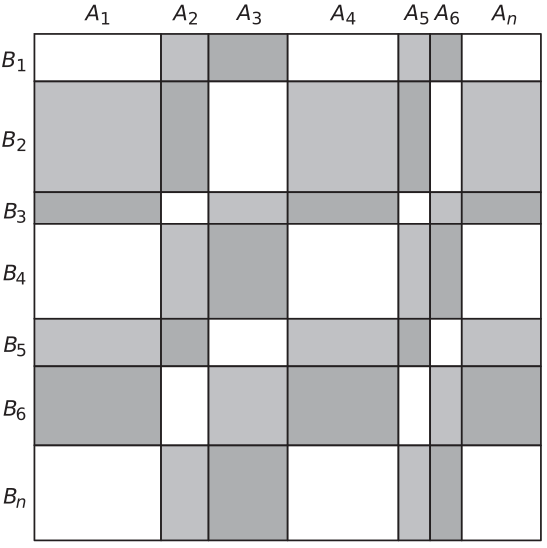
\includegraphics[scale=.25]{frosting_on_cake}
		\caption{An instance of the problem \textit{Frosting on the Cake}.}
	\end{figure}
	\noindent To prepare the frosting, Iskander wants to know the total surface in square centimeters to be colored for each of the 3 colors, \& asks for your help.
	\begin{itemize}
		\item {\sf Input.} The input consists of the following integers: on the 1st line: the integer $n\in\mathbb{N}^\star$, on the 2nd line: the values of $A_1,A_2,\ldots,A_n,n$ integers separated by single spaces, on the 3rd line: the values of $B_1,B_2,\ldots,B_n,n$ integers separated by single spaces.
		\item {\sf Limits.} The input satisfies $3\le n\le100000$ \& $1\le A_i,B_i\le10000$, $i = 1,2,\ldots,n$.
		\item {\sf Output.} The output should consist of 3 integers separated by single spaces, representing the total area for each color $0,1,2$.
	\end{itemize}
\end{problem}

\begin{proof}[Solution]
	Followed \cite[Sect. 1.8, pp. 39--41]{Durr_Vie2021}, we want to find a solution that runs in time $O(n)$ or possibly $O(n\log n)$, which rules out the naive solution which loops over all $n^2$ grid cells \& accumulates their areas in variables corresponding to each color. Permuting columns or rows preserves the total area of each color. Hence, we can reduce to the $n = 3$ case, by simply summing the values of each color class $A_{3k},A_{3k+1},A_{3k+2}$. Then the answer per color class is just the sum of the areas of 3 rectangles. The tricky part relies in not mixing up the colors.
\end{proof}

\begin{Verbatim}[numbers=left,xleftmargin=5mm]
	def read_ints(): return [int(x) for x in input().split()]
	def cat(l): return tuple(sum(l[n::3]) for n in [1, 2, 0])
	input() # n
	A = cat(read_ints())
	B = cat(read_ints())
	print("{} {} {}".format(B[2] * A[0] + B[0] * A[2] + B[1] * A[1],
	B[2] * A[1] + B[0] * A[0] + B[1] * A[2],
	B[2] * A[2] + B[0] * A[1] + B[1] * A[0]))
\end{Verbatim}

\begin{baitoan}[\cite{Trung_HSG_THPT_Tin}, 1., p. 13, HSG Lớp 10 Vĩnh Phúc 2020--2021, Square -- Hình vuông]
	Cho $n$ điểm có tọa độ là các số nguyên trên hệ trục tọa độ $Oxy$. Tìm diện tích hình vuông nhỏ nhất có các cạnh song song với các trục tọa độ sao cho tất cả các điểm đã cho đều thuộc hình vuông đó (điểm nằm trên cạnh hình vuông cũng được coi là thuộc hình vuông đó).
	\begin{itemize}
		\item {\sf Input.} Dòng 1: chứa số nguyên dương $n\in\mathbb{N}^\star$, $2\le n\le20$, là số lượng điểm có tọa độ là các số nguyên. $n$ dòng tiếp theo, mỗi dòng ghi 2 số nguyên $x,y\in\mathbb{Z}$, $1\le x,y\le100$, là tọa độ của mỗi điểm.
		\item {\sf Output.} Ghi diện tích hình vuông nhỏ nhất tìm được.
		\item {\sf Sample.}
		\begin{table}[H]
			\centering
			\begin{tabular}{|l|l|}
				\hline
				{\tt square.inp} & {\tt square.out} \\
				\hline
				3 & 16 \\
				3 4 &  \\
				5 7 &  \\
				4 3 &  \\
				\hline
			\end{tabular}
		\end{table}
	\end{itemize}
\end{baitoan}
\noindent Pascal:

Python: \url{https://github.com/NQBH/hobby/blob/master/elementary_computer_science/Python/square.py}.
\begin{Verbatim}[numbers=left,xleftmargin=5mm]
	# 1st solution. Author: NQBH
	def square():
	n = int(input())
	a = [0]*n
	b = [0]*n
	for i in range(n):
	tmp = input()
	tmp = tmp.split()
	a[i] = int(tmp[0])
	b[i] = int(tmp[1])
	max_diff = 0
	for i in range(n):
	for j in range(i + 1, n):
	if abs(a[i] - a[j]) > max_diff:
	max_diff = abs(a[i] - a[j])
	if abs(b[i] - b[j]) > max_diff:
	max_diff = abs(b[i] - b[j])
	print(max_diff**2)
	square()
	# 2nd solution. Author: Vuong Thanh Trung
	inf = 1000
	xmin = inf
	xmax = -inf
	ymin = inf
	ymax = -inf
	file = open("square.inp", "r")
	n = int(file.readline())
	for i in range(n):
	x, y = map(int, file.readline().split())
	xmin = min(xmin, x)
	xmax = max(xmax, x)
	ymin = min(ymin, y)
	ymax = max(ymax, y)
	file.close()
	file = open("square.out", "w")
	c = max(xmax - xmin, ymax - ymin)
	file.write(str(c*c))
	file.close()
\end{Verbatim}
C++: \url{https://github.com/NQBH/hobby/blob/master/elementary_computer_science/Cpp/square.cpp}.
\begin{Verbatim}[numbers=left,xleftmargin=5mm]
	#include <bits/stdc++.h>
	#define inf 1000
	using namespace std;
	int xmin = inf, ymin = inf, xmax = -inf, ymax = -inf;
	int n;
	int main() {
		freopen("square.inp", "r", stdin);
		freopen("square.out", "w", stdout);
		cin >> n;
		for (int i = 1; i <= n; ++i) {
			int x, y;
			cin >> x >> y;
			xmin = min(xmin, x);
			xmax = max(xmax, x);
			ymin = min(ymin, y);
			ymax = max(ymax, y);
		}
		int c = max(xmax - xmin, ymax - ymin);
		cout << c*c;
		return 0;
	}
	// Terminal: g++ -std=c++11 -O2 -Wall square.cpp -o square
\end{Verbatim}

\begin{luuy}
	Nếu yêu cầu của bài toán trên đổi từ `hình vuông' sang `hình chữ nhật' thì:
	\begin{Verbatim}[numbers=left,xleftmargin=5mm]
		cout << (xmax - xmin)*(ymax - ymin);
	\end{Verbatim}
\end{luuy}
Bài toán này có thể mở rộng từ 2D sang 3D:

\begin{baitoan}[Mở rộng \cite{Trung_HSG_THPT_Tin}, 1., p. 13, HSG Lớp 10 Vĩnh Phúc 2020--2021, Square -- Hình vuông]
	Cho $n$ điểm có tọa độ là các số nguyên trên hệ trục tọa độ $Oxyz$. Tìm diện tích hình chữ nhật \& lập phương nhỏ nhất có các cạnh song song với các trục tọa độ sao cho tất cả các điểm đã cho đều thuộc hình vuông đó (điểm nằm trên cạnh hình chữ nhật hoặc hình vuông cũng được coi là thuộc hình vuông đó).
	\begin{itemize}
		\item {\sf Input.} Dòng 1: chứa số nguyên dương $n\in\mathbb{N}^\star$, $2\le n\le20$, là số lượng điểm có tọa độ là các số nguyên. $n$ dòng tiếp theo, mỗi dòng ghi 3 số nguyên $x,y,z\in\mathbb{Z}$, $1\le x,y,z\le100$, là tọa độ của mỗi điểm.
		\item {\sf Output.} Ghi diện tích hình vuông nhỏ nhất tìm được.
		\item {\sf Sample.}
		\begin{table}[H]
			\centering
			\begin{tabular}{|l|l|}
				\hline
				{\tt square.inp} & {\tt square.out} \\
				\hline
				3 &  \\
				3 4 1 &  \\
				5 7 -8 &  \\
				4 3 9 &  \\
				\hline
			\end{tabular}
		\end{table}
	\end{itemize}
\end{baitoan}

\begin{baitoan}[\cite{Trung_HSG_THPT_Tin}, 2., pp. 13--14, HSG Lớp 10 Vĩnh Phúc 2020--2021, Divisible by 3 -- Chia hết cho 3]
	Cho dãy $a$ gồm $n$ số nguyên dương. Cho biết có bao nhiêu cặp số trong dãy có tổng chia hết cho $3$, i.e., đếm xem có bao nhiêu cặp chỉ số $i,j$, $1\le i < j\le n$, sao cho $a_i + a_j\divby3$.
	\begin{itemize}
		\item {\sf Input.} Dòng 1: 1 số nguyên duy nhất $n$, $1\le n\le10^5$. Dòng 2: Ghi $n$ số nguyên dương $a_1,a_2,\ldots,a_n$, $1\le a_i\le10^5$, $\forall i = 1,2,\ldots,n$, là các phần tử của dãy.
		\item {\sf Output.} 1 dòng duy nhất ghi số lượng cặp số của dãy $a$ có tổng chia hết cho $3$.
		\item {\sf Sample.}
		\begin{table}[H]
			\centering
			\begin{tabular}{|l|l|l|}
				\hline
				{\tt div3.inp} & {\tt div3.out} & Giải thích \\
				\hline
				5 & 3 & 3 cặp số tìm được có chỉ số: $(1,4),(2,3),(3,5)$. \\
				3 6 9 12 & & \\
				\hline
				4 & 6 & 6 cặp số tìm được có chỉ số: $(1,2),(1,3),(1,4),(2,3),(2,4),(3,4)$. \\
				3 6 9 12 & & \\
				\hline
			\end{tabular}
		\end{table}
	\end{itemize}
\end{baitoan}
Python:
\begin{itemize}
	\item \url{https://github.com/NQBH/hobby/blob/master/elementary_computer_science/Python/div3.py}.
	\item \url{https://github.com/NQBH/hobby/blob/master/elementary_computer_science/Python/div3_io.py}.
\end{itemize}
\begin{Verbatim}[numbers=left,xleftmargin=5mm]
	file = open("div3.inp", "r")
	n = int(file.readline())
	a = list(map(int, file.readline().split()))
	c = [0, 0, 0]
	for x in a:
	c[x % 3] += 1
	file.close()
	res = (c[0]*(c[0] - 1)) // 2 + c[1]*c[2]
	file = open("div3.out", "w")
	file.write(str(res))
	file.close()
\end{Verbatim}
C++: \url{https://github.com/NQBH/hobby/blob/master/elementary_computer_science/Cpp/div3.cpp}.
\begin{Verbatim}[numbers=left,xleftmargin=5mm]
	#include <bits/stdc++.h>
	using namespace std;
	int n, x, c[3];
	long long res;
	int main() {
		freopen("div3.inp", "r", stdin);
		freopen("div3.out", "w", stdout);
		cin >> n;
		for (int i = 1; i <= n; ++i) {
			cin >> x;
			++c[x % 3];
		}
		res = (c[0]*(c[0] - 1))/2 + c[1]*c[2];
		cout << res;
		return 0;
	}
	// Terminal: g++ -std=c++11 -O2 -Wall div3.cpp -o div3
\end{Verbatim}

%------------------------------------------------------------------------------%

\subsection{Google Kickstart Round A 2020}
Watch \href{https://www.youtube.com/watch?v=uGrBHohIgQY}{YouTube{\tt/}William Lin{\tt/}Winning Google Kickstart Round A 2020}.

\begin{problem}[Google Kickstart Round A 2020, Allocation]
	There are $n$ houses for sale. The $i$th house costs $a_i$ dollars to buy. You have a budget of $b$ dollars to spend. What is the maximum number of houses you can buy?
	\begin{itemize}
		\item {\sf Input.} The 1st line of the input gives the number of test cases, $t$. $t$ test cases follow. Each test case begins with a single line containing the 2 integers $n,b$. The 2nd line contains $n$ integers. The $i$th integer is $a_i$, the cost of the $i$th house.
		\item {\sf Output.} For each test case, output 1 line containing \verb|Case #x: y|, where {\tt x} is the test case number (starting from $1$) \& {\tt y} is the maximum number of houses you can buy.
		\item {\sf Limits:} Time limit: \emph{15 s{\tt/}test set}. Memory limit: \emph{1GB}. $1\le t\le100$, $1\le b\le10^5$, $1\le a_i\le1000$, $\forall i = 1,2,\ldots,n$. Test set 1: $1\le n\le100$. Test set 2: $1\le n\le10^5$.
		\item {\sf Sample.}
		\begin{table}[H]
			\centering
			\begin{tabular}{|l|l|}
				\hline
				{\tt allocation.inp} & {\tt allocation.out} \\
				\hline
				3 & Case \#1: 2 \\
				4 100 & Case \#2: 3 \\
				20 90 40 90 & Case \#3: 0 \\
				4 50 & \\
				30 30 10 10 & \\
				3 300 & \\
				999 999 999 & \\
				\hline
			\end{tabular}
		\end{table}
	\end{itemize}
\end{problem}

\begin{Verbatim}[numbers=left,xleftmargin=5mm]
	#include <bits/stdc++.h>
	using namespace std;
	int n, b, a[100000];
	
	void solve() {
		cout << "Enter n: ";
		cin >>  n;
		cout << "Enter b: ";
		cin >>  b;
		cout << "Enter array a: ";
		for(int i = 0; i < n; ++i)
		cin >> a[i];
		sort(a, a + n);
		int ans = 0;
		for (int i = 0; i < n; ++i) {
			if (b >= a[i]) {
				b -= a[i];
				++ ans;
			}
		}
		cout << ans << "\n";
	}
	
	int main() {
		int t, i = 1;
		cout << "Enter t: ";
		cin >> t;
		while (t--) {
			cout << "Case #" << i << ": ";
			solve();
			++i;
		}
	}
\end{Verbatim}

\begin{problem}[Google Kickstart Round A 2020, Plates]
	Dr. Patel has $n$ stacks of plates. Each stack contains $k$ plates. Each plate has a positive beauty value, describing how beautiful it looks. Dr. Patel would like to take exactly $p$ plates to use for dinner tonight. If he would like to take a plate in a stack, he must also take all of the plates above it in that stack as well. Help Dr. Patel pick the $p$ plates that would maximize the total sum of beauty values.
	\begin{itemize}
		\item {\sf Input.} The 1st line of the input gives the number of test cases, $t$. $t$ test cases follow. Each test case begins with a line containing the 3 integers $n,k,p$. Then, $n$ lines follow. The $i$th line contains $k$ integers, describing the beauty values of each stack of plates from top to bottom.
		\item {\sf Output.} For each test case, output 1 line containing \verb|Case #x: y|, where {\tt x} is the test case number (starting from $1$) \& {\tt y} is the maximum total sum of beauty values that Dr. Patel could pick.
		\item {\sf Limits:} Time limit: \emph{20 s{\tt/}test set}. Memory limit: \emph{1GB}. $\le t\le100$, $1\le k\le30$, $1\le p\le nk$. The beauty values are between $1$ \& $100$, inclusive. Test set 1: $1\le n\le 3$. Test set 2: $1\le n\le50$.
		\item {\sf Sample.}
		\begin{table}[H]
			\centering
			\begin{tabular}{|l|l|}
				\hline
				{\tt plate.inp} & {\tt plate.out} \\
				\hline
				2 & Case \#1: 250 \\
				2 4 5 & Case \#2: 180 \\
				10 10 100 30 & \\
				80 50 10 50 & \\
				3 2 3 & \\
				80 80 & \\
				15 50 & \\
				20 10 & \\
				\hline
			\end{tabular}
		\end{table}
	\end{itemize}
\end{problem}

%------------------------------------------------------------------------------%

\section{CSES Problem Set}

\begin{problem}[Weird Algorithm]
	Consider an algorithm that takes as input a positive integer $n\in\mathbb{N}^\star$. If $n$ is even, the algorithm divides it by $2$, \& if $n$ is odd, the algorithm multiplies it by $3$ \& adds $1$. The algorithms repeats this, until $n$ is $1$. E.g., the sequence for $n = 3$ is as follows: $3\to10\to5\to16\to8\to4\to2\to1$. Your task is to simulate the execution of the algorithm for a given value of $n$.
	\begin{itemize}
		\item {\sf Input.} The only input line contains an integer $n\in\mathbb{Z}$.
		\item {\sf Output.} Print a line that contains all values of $n$ during the algorithm.
		\item {\sf Constraints.} $1\le n\le10^6$.
		\item {\sf Sample.}
		\begin{table}[H]
			\centering
			\begin{tabular}{|l|l|}
				\hline
				\verb|weird_algorithm.inp| & \verb|weird_algorithm.out| \\
				\hline
				3 & 3 10 5 16 8 4 2 1 \\
				\hline
			\end{tabular}
		\end{table}
	\end{itemize}
\end{problem}
Source: \href{https://cses.fi/problemset/task/1068}{CSES Problem Set{\tt/}weird algorithm}, \& \cite[Sect. 1.3, pp. 5--7]{Laaksonen2020}.

\begin{Verbatim}[numbers=left,xleftmargin=5mm]
	#include <iostream>
	using namespace std;
	
	int main() {
		long long n;
		cin >> n;
		while (1) {
			cout << n << " ";
			if (n == 1) break;
			if (n%2 == 0) n /= 2;
			else n = n*3 + 1;
		}
		cout << "\n";
	}
\end{Verbatim}

\begin{remark}[Collatz conjecture]
	The above algorithm terminates $\forall n\in\mathbb{N}^\star$.
\end{remark}

\begin{problem}[Missing Number]
	You are given all numbers between $1,2,\ldots,n$ except one. Your task is to find the missing number.
	\begin{itemize}
		\item {\sf Input.} The 1st input line contains a positive integer $n\in\mathbb{N}^\star$. The 2nd line contains $n - 1$ numbers. Each number is distinct \& between $1$ \& $n$ (inclusive).
		\item {\sf Output.} Print the missing number.
		\item {\sf Constraints.} $2\le n\le2\cdot10^5$.
		\item {\sf Sample.}
		\begin{table}[H]
			\centering
			\begin{tabular}{|l|l|}
				\hline
				\verb|missing_number.inp| & \verb|missing_number.out| \\
				\hline
				5 & 4 \\
				2 3 1 5 & \\
				\hline
			\end{tabular}
		\end{table}
	\end{itemize}
\end{problem}
Source: \href{https://cses.fi/problemset/task/1083}{CSES Problem Set{\tt/}missing number}.

\begin{Verbatim}[numbers=left,xleftmargin=5mm]
	file_in = open("missing_number.inp")
	file_out = open("missing_number.out", "w")
	n = int(file_in.readline())
	data = file_in.readline()
	A = data.split()
	A = [int(i) for i in A]
	A.sort()
	for i in range(n-1):
	if i + 1 != A[i]:
	file_out.write(str(i + 1))
	break
	file_in.close()
	file_out.close()
\end{Verbatim}

\begin{problem}[Repetitions]
	You are given a DNA sequence: a string consisting of characters A, C, G, \& T. Your task is to find the longest repetition in the sequence. This is a maximum-length substring containing only 1 type of character.
	\begin{itemize}
		\item {\sf Input.} The only input line contains a string of $n\in\mathbb{N}^\star$ characters.
		\item {\sf Output.} Print 1 integer: the length of the longest repetition.
		\item {\sf Constraints.} $1\le n\le10^6$.
		\item {\sf Sample.}
		\begin{table}[H]
			\centering
			\begin{tabular}{|l|l|}
				\hline
				\verb|repetition.inp| & \verb|repetition.out| \\
				\hline
				ATTCGGGA & 3 \\
				\hline
			\end{tabular}
		\end{table}
	\end{itemize}	
\end{problem}
Source: \href{https://cses.fi/problemset/task/1069}{CSES problem Set{\tt/}repetition}.

\begin{Verbatim}[numbers=left,xleftmargin=5mm]
	DNA = input()
	DNA_count = []
	count = 1
	char = DNA[0]
	for i in range(1, len(DNA)):
	if DNA[i] == DNA[i-1]:
	count = count + 1
	else:
	DNA_count.append(count)
	count = 1
	DNA_count.append(count)
	print(max(DNA_count))
\end{Verbatim}

\begin{problem}[Non-decreasing Array]
	You are given an array of $n$ integers. You want to modify the array so that it is non-decreasing, i.e., every element is at least as large as the previous element. On each move, you may increase the value of any element by $1$. What is the minimum number of moves required?
	\begin{itemize}
		\item {\sf Input.} The 1st input line contains an integer $n$: the size of the array. The 2nd line contains $n$ integers $x_1,x_2,\ldots,x_n$: the contents of the array.
		\item {\sf Output.} Print the minimum number of moves.
		\item {\sf Constraints.} $1\le n\le2\cdot10^5$, $1\le x_i\le10^9$.
		\item {\sf Sample.}
		\begin{table}[H]
			\centering
			\begin{tabular}{|l|l|}
				\hline
				\verb|nondecreasing_array.inp| & \verb|nondecreasing_array.out| \\
				\hline
				5 & 5 \\
				3 2 5 1 7 & \\
				\hline
			\end{tabular}
		\end{table}
	\end{itemize}
\end{problem}
Source: \href{https://cses.fi/problemset/task/1094}{CSES problem Set{\tt/}increasing array}.

\begin{Verbatim}[numbers=left,xleftmargin=5mm]
	n = int(input())
	A = input()
	A = A.split()
	A = [int(i) for i in A]
	ans = 0
	for i in range(1, len(A)):
	if A[i] < A[i - 1]:
	ans = ans + A[i-1] - A[i]
	A[i] = A[i - 1]
	print(ans)
\end{Verbatim}

\begin{problem}[Permutations]
	A permutation of integers $1,2,\ldots,n$ is called \emph{beautiful} if there are no adjacent elements whose difference is $1$. Given $n$, construct a beautiful permutation if such a permutation exists.
	\begin{itemize}
		\item {\sf Input.} The only input line contains an integer $n$.
		\item {\sf Output.} Print a beautiful permutation of integers $1,2,\ldots,n$. If there are several solutions, you may print any of them. If there are no solutions, print \verb|"NO SOLUTION"|.
		\item {\sf Constraints.} $1\le n\le10^6$.
		\item {\sf Sample.}
		\begin{table}[H]
			\centering
			\begin{tabular}{|l|l|}
				\hline
				\verb|permutations.inp| & \verb|permutations.out| \\
				\hline
				5 & 4 2 5 3 1 \\
				\hline
				3 & NO SOLUTION \\
				\hline
			\end{tabular}
		\end{table}
	\end{itemize}
\end{problem}

\begin{Verbatim}[numbers=left,xleftmargin=5mm]
	n = int(input())
	A = [1]
	if n == 1:
	print(1)
	elif n == 2 or n == 3:
	print("NO SOLUTION")
	elif n == 4:
	print("2 4 1 3")
	else:
	for i in range(1, n):
	tmp = A[i-1] + 2
	if tmp <= n:
	A.append(tmp)
	else:
	A.append(2)
	print(*A)
\end{Verbatim}

\begin{problem}[Number Spiral]
	A \emph{number spiral} is an infinite grid whose upper-left square has number $1$. Here are the 1st 5 layers of the spiral:
	\begin{table}[H]
		\centering
		\begin{tabular}{|c|c|c|c|c|}
			\hline
			1 & 2 & 9 & 10 & 25 \\
			\hline
			4 & 3 & 8 & 11 & 24 \\
			\hline
			5 & 6 & 7 & 12 & 23 \\
			\hline
			16 & 15 & 14 & 13 & 22 \\
			\hline
			17 & 18 & 19 & 20 & 21 \\
			\hline
		\end{tabular}
	\end{table}
	Your task is to find out the number in row $y$ \& column $x$.
	\begin{itemize}
		\item {\sf Input.} The 1st input line contains an integer $t$: the number of tests. After this, there are $t$ lines, each containing integers $y,x$.
		\item {\sf Output.} For each test, print the number in row $y$ and column $x$.
		\item {\sf Constraints.} $1\le t\le10^5$, $1\le x,y\le10^9$.
		\item {\sf Sample.}
		\begin{table}[H]
			\centering
			\begin{tabular}{|l|l|}
				\hline
				\verb|number_spiral.inp| & \verb|number_spiral.out| \\
				\hline
				3 & 8 \\
				2 3 & 1 \\
				1 1 & 15 \\
				4 2 & \\
				\hline				
			\end{tabular}
		\end{table}
	\end{itemize}
\end{problem}

%------------------------------------------------------------------------------%

\printbibliography[heading=bibintoc]

\end{document}